\documentclass[a4paper, 12pt]{article}
\usepackage{bmstu-title-new}
\usepackage{pdfpages}
\usepackage{acronym}
\usepackage{totcount}
\usepackage[export]{adjustbox}

\setcounter{tocdepth}{3}
\setcounter{secnumdepth}{4}

\addbibresource{src/bibliography.bib}

% Подсчет общего количества источников
\newtotcounter{citenum}
\AtEveryBibitem{\stepcounter{citenum}}

\newtotcounter{pagecount}
\newtotcounter{appendixcount}
\newtotcounter{figurescount}

\workname{Программно-аппаратная система бесконтактной оплаты}
\discipline{Микропроцессорные системы}
\group{ИУ6-84Б}
\author{С. А. Рахманов}
\tutor[Руководитель]{С. А. Хохлов}
\inspector[Нормоконтролер]{О. Ю. Ерёмин}

\newboolean{test_vkr}
\setboolean{test_vkr}{false}

\newboolean{website_upload}
\setboolean{website_upload}{false}

\begin{document}
	\ifthenelse{\boolean{website_upload}}{
		%
\includepdf{docs/titul.pdf} %титульный лист РПЗ
		%
\includepdf{docs/podpis/zadanie.pdf} % задание на ВКР
		%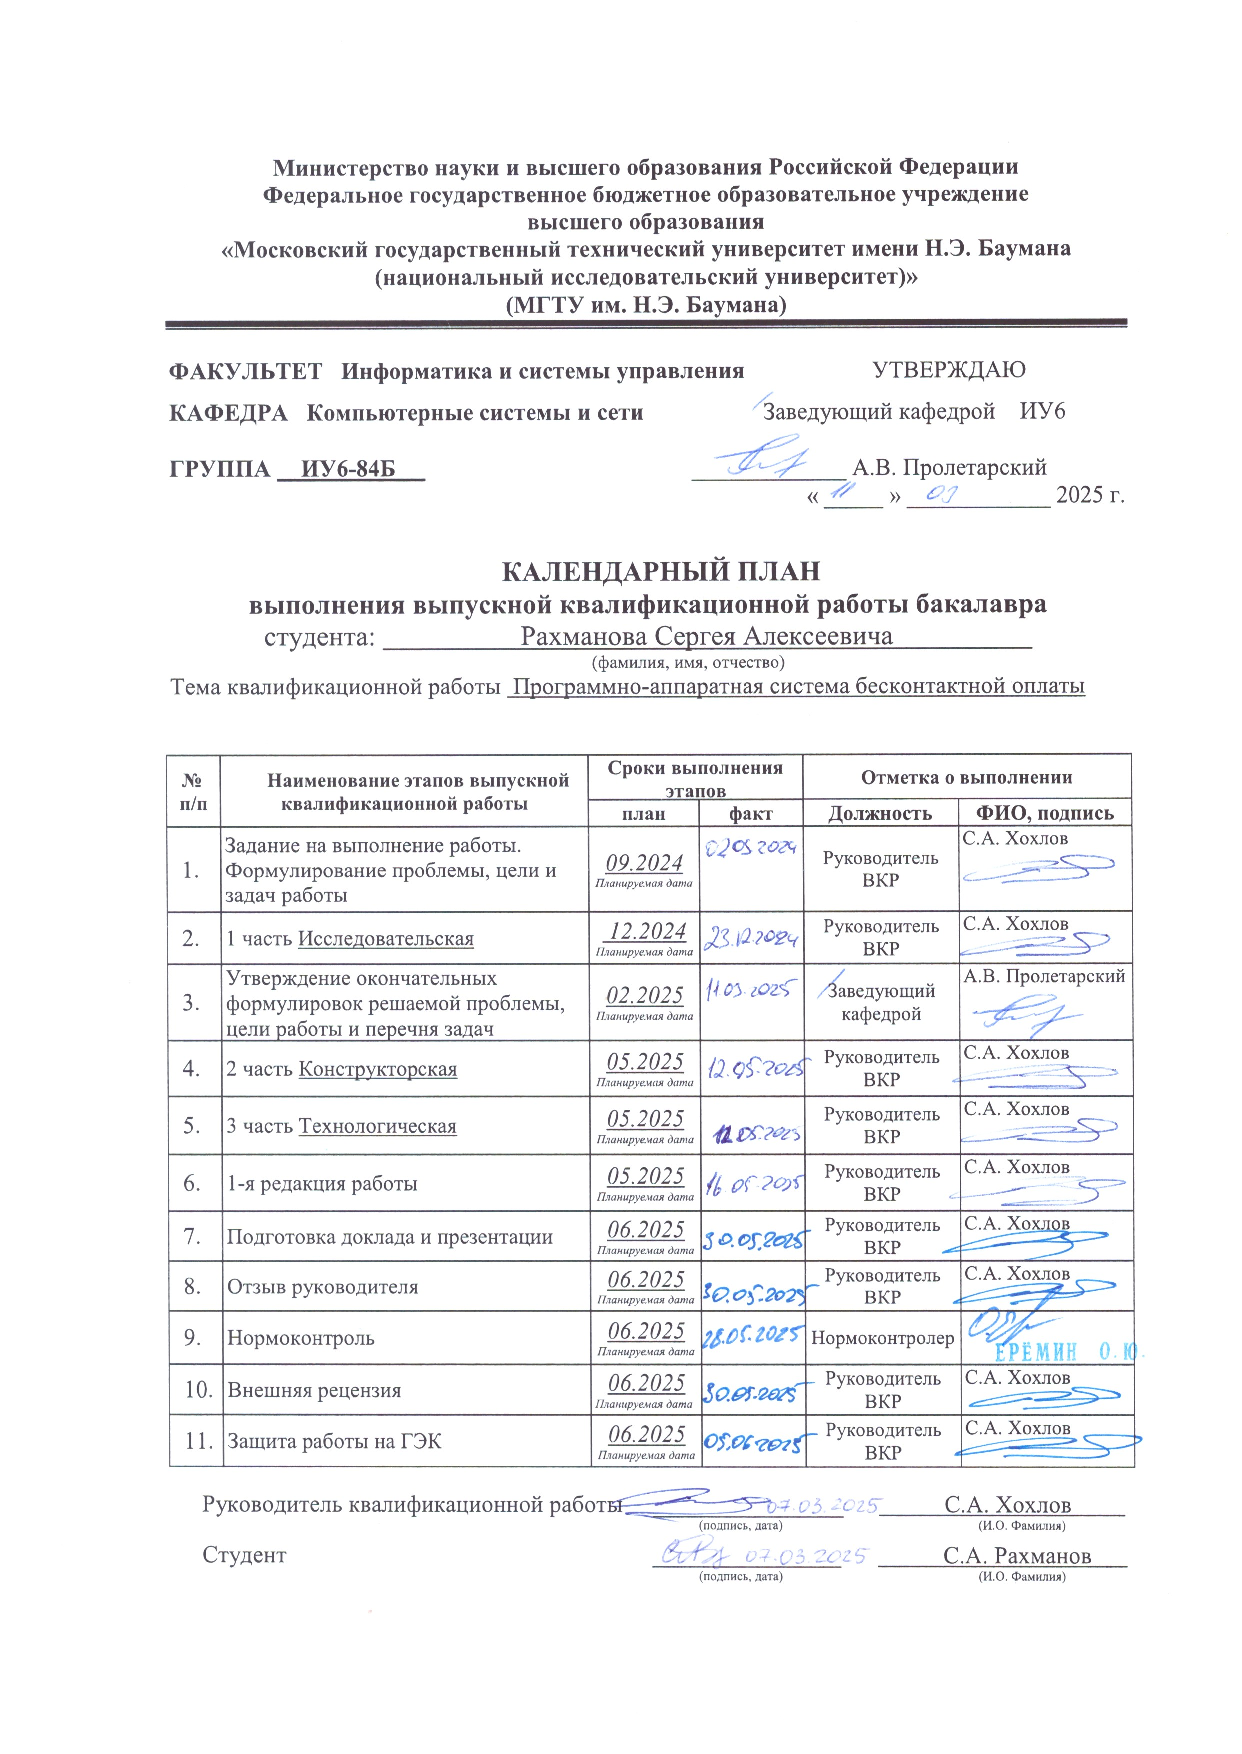
\includepdf{docs/plan.pdf}
		\setcounter{page}{4}
		%\large %TODO al: fix bmstu title which enlarge font size
	} {
		\bmstutitleDiploma
		\setcounter{page}{2}
	}

	\newpage

\centeredsection{АННОТАЦИЯ}

Настоящая расчетно-пояснительная записка к выпускной квалификационной работе бакалавра посвящена процессу создания программно-аппаратной системы бесконтактной оплаты.

В процессе выполнения работы был проведен анализ технологий осуществления бесконтактной оплаты, методов и инструментов ее реализации. 
Помимо этого были проанализированы аналоги данной системы.
В результате выполнения анализа были установлены требования к разрабатываемой системе: ее аппаратной и программной частям.

На основании требований была спроектирована программно-аппаратная система, включающая в себя устройство-терминал для взаимодействия с платежным средством и управляющая программа для мобильного устройства пользователя под управлением ОС Android.

\begin{center}
  \textbf{ABSTRACT}
\end{center}

This calculation and explanatory note to the bachelor's graduate qualification work is devoted to the process of creating a hardware-software system of contactless payment.

In the process of work implementation technologies of contactless payment, methods and tools of its implementation were analyzed. 
In addition, analogues of this system were analyzed.
Requirements to the developed system, its hardware and software parts were established according to the results of the analysis.

A hardware-software system was designed based on the requirements, including a terminal device for interaction with the payment medium and a control program for the user's mobile device running Android OS.
	
	\newpage

\begin{center}
	\textbf{РЕФЕРАТ}
\end{center}

Записка на~\pageref{LastPage} с. (без учета приложений~\total{pagecount} с.), \total{figurescount} рис., \totaltables{} табл., \total{citenum} источников, \total{appendixcount} приложений.

БЕСКОНТАКТНАЯ ОПЛАТА, ПЛАТЕЖНЫЙ ТЕРМИНАЛ, МОБИЛЬНЫЕ ПЛАТЕЖИ, ЭКВАЙРИНГ, NFC, Android, STM32, SPI, USART.

Объектом разработки данной выпускной квалификационной работы бакалавра является программно-аппаратная система бесконтактной оплаты.

Цель работы~--- программно-аппаратная система, позволяющая интегрироваться с платежной системой банка и принимать оплату бесконтактными средствами платежа (банковскими картами и устройствами с поддержкой бесконтактной оплаты на территории Российской Федерации).

В процессе выполнения работы были выполнены следующие задачи: анализ технологий работы платежного терминала, проектирование и определение спецификаций аппаратной и программной частей системы, разработка и тестирование программного обеспечения системы, создание макета системы, тестирование системы и интеграции между ее частями.

В результате была спроектирована, разработана и протестирована программно-аппаратная система бесконтактной оплаты.
Пользователями данной системы являются банки и финансовые организации, предоставляющие услуги эквайринга.

	
	\newpage
	\begin{centering}
		% меняем формат заголовка на корректный для структурного элемента
		\titleformat{\section}
			{\normalfont\fontsize{15}{16}\selectfont\bfseries\centering}{}{0pt}{}

		\tableofcontents

		% возвращаем формат заголовка
		\titleformat{\section}
			{\normalfont\fontsize{15}{16}\selectfont\bfseries}{\thesection}{0.5em}{} % один пробел между номером и заголовком

	\end{centering}

	\newpage

\centeredsection{ОПРЕДЕЛЕНИЯ, ОБОЗНАЧЕНИЯ И СОКРАЩЕНИЯ}
\addcontentsline{toc}{section}{ОПРЕДЕЛЕНИЯ, ОБОЗНАЧЕНИЯ И СОКРАЩЕНИЯ}

В настоящей работе применяются следующие сокращения и обозначения:

% TODO: обновить список в соответствии с содержанием
\begin{description}

	\item МК~--- микроконтроллер;
	\item ПО~--- программное обеспечение;
	\item ПС~--- платежная система;
	\item СБО~--- система бесконтактной оплаты;
	\item ТСП~--- торгово-сервисные предприятия;

	\item EMV~--- технический стандарт для пластиковых карт, совместно разработанный платежными системами Europay, Mastercard и Visa;
	\item GPIO (General Purpose Input/Output)~--- интерфейс ввода/вывода общего назначения;
	\item NFC (Near Field Communication)~--- технология беспроводной передачи данных малого радиуса действия, которая даёт возможность обмена данными между устройствами, находящимися на расстоянии около 10 сантиметров;
	\item PCD (Proximity Coupling Device)~--- устройство считывания, предназначенное для взаимодействия с бесконтактными картами;
	\item PICC (Proximity Integrated Circuit Card)~--- бесконтактная карта с интегральной схемой, предназначенная для взаимодействия с устройством считывания на малом расстоянии;
	\item PIN (Personal identification number)~--- персональный идентификационный номер;
	\item POS-терминал (Point Of Sale терминал)~--- аппаратное устройство, используемое для осуществления платежей по банковским картам;
	\item UART (Universal Asynchronous Receiver-Transmitter)~--- универсальный асинхронный приемопередатчик.

\item \end{description}

	
	\newpage

\centeredsection{ВВЕДЕНИЕ}
\addcontentsline{toc}{section}{ВВЕДЕНИЕ}

Бесконтактные платежи – это современный способ безналичной оплаты, который стал неотъемлемой частью повседневной жизни.
Их преимущество очевидно из названия --- они не требуют физического контакта карты с терминалом, в результате чего ускоряется процесс выполнения оплаты и повышается скорость и качество обслуживания, особенно при покупках на небольшую сумму, когда нет необходимости вводить PIN-код карты.

Однако бесконтактный метод оплаты имеет свои нюансы: для его работы нужен платежный терминал, поддерживающий данную технологию, также при оплате на небольшие суммы карта не требует ввода пин-кода, поэтому любой человек может воспользоваться ей для оплаты, а также есть риск подмены платежного терминал мошенниками~\cite{codejournal}.
Несмотря на это бесконтактная оплата является наиболее распространенным способом оплаты как на глобальном, так и на российском рынке~\cite{posterminals}.
Согласно данным Банка России и Национальной системы платежных карт (НСПК), число операций с использованием бесконтактных технологий ежегодно увеличивается, и в 2024-м году доля безналичных платежей в розничном обороте составила 85,8\%,
Самым популярным средством безналичной оплаты оставались платежные карты
~\cite{cdrf_report2024,cdrf_results2024}.
Что свидетельствует о высоком уровне доверия со стороны потребителей и ритейлеров и делает особенно актуальным разработку собственных решений бесконтактной оплаты, адаптированных под локальные требования и стандарты, а также обладающих гибкой архитектурой для дальнейшего масштабирования и интеграции.

На сегодняшний день существует множество коммерческих решений, предоставляющих возможность приема бесконтактных платежей.
Однако большинство из них ориентировано на крупные предприятия и требуют значительных финансовых и технических затрат при внедрении.
Таким образом, возникает потребность в создании компактной и экономически эффективной программно-аппаратной системы бесконтактной оплаты, которая может быть использована как малым бизнесом, так и частными лицами в условиях ограниченного бюджета.


Актуальность настоящей работы заключается в том, что современный рынок нуждается в доступных и простых в использовании решениях для организации бесконтактной оплаты, способных интегрироваться с существующими платежными системами и соответствовать всем необходимым требованиям безопасности.
Такие системы должны обеспечивать простоту установки, минимальное время настройки и устойчивость к внешним воздействиям в различных условиях эксплуатации.


Целью данной работы является проектирование и реализация программно-аппаратной системы бесконтактной оплаты (СБО), которая могла бы интегрироваться с платежной системой банка и позволяла принимать оплату бесконтактными средствами платежа (банковскими картами и устройствами с поддержкой бесконтактной оплаты на территории Российской Федерации).
СБО состоит из устройства для взаимодействия со средством платежа (мобильный терминал бесконтактной оплаты) и мобильного приложения для управления платежной транзакцией путем взаимодействия с платежным сервисом и мобильным терминалом.


	\newpage

% Из текста короткого задания на ВКР:
% 1. Проанализировать технологии, используемые для реализации бесконтактного взаимодействия платежного терминала и средства платежа (карты, смартфона и пр.).
% 2. Проанализировать методы и инструменты обеспечения безопасности бесконтактных платежей
% -. Сравнение существующих аналогов систем коррекции
% -. Выбор методы и технологий разработки системы


%  - Как технически выглядит процесс оплаты (от введения суммы и прикладывания карты, до отображения статуса платежа)
%  - Декомпозиция процесса на технологии, используемые на разных этапах
%  - Обзор технологий
%    - с точки зрения тех. процесса
%    - с точки зрения безопасности
%  - Сравнительный анализ существующих решений
%  - Формирование требований к системе (используемые технологии, превосходство над аналогами)

\section{Анализ предметной области}

\subsection{Развитие сферы банковских платежей}

\subsubsection{Развитие платежных операций}

Появление банковской системы, выступающей в качестве посредника между государством и гражданами, ознаменовало процесс непрерывного развития финансовых технологий, поскольку банки стремились повысить свою прибыльность, в том числе путем повышения качества платежных сервисов.
Деньги выступали в качестве основного способа оплаты товаров и услуг, однако не всегда были удобным способом оплаты, поэтому в дополнение к ним сначала появились бумажные чеки, а позднее и банковские карты.
Вместе с появлением банковских карт, появились и платежные системы~-- инстанции, которые не только выпускали и поддерживали карты, но и выступали посредниками между банками.
Для приема карт к оплате необходимы были специальные устройства.
Изначально это были импринтер, с помощью которого создавались слипы~-- бумаги, содержащие реквизиты карты, дату и сумму покупки и др..
Ему на смену пришел электронный терминал оплаты (POS-терминал), который упрощал взаимодействие с картой, т.к. передавал информацию о карте напрямую в процессиноговые центры платежной системы.

При приеме карты кассир должен был получить информацию от банка, что у держателя карты есть необходимый объем денежных средств для оплаты, в противном случае товар или услуга не могла быть оплачена.
Изначально этот процесс выглядел следующим образом: кассир звонил в банк-эквайер, тот связывался с банком-эмитентом, выпустившем карту, который подтверждал наличие необходимой суммы и инициировал ее передачу в банк-эквайер либо сообщал о невозможности оплаты.
Платежные системы изначально выступали каналом связи между банками.
Однако с увеличением количества карт создавалась высокая нагрузка на банки, и с целью ее снижения появились специальные процессинговые центры, которые совместно с платежными системами осуществляли функцию клиринга~\cite{habr_fondy_payment_history}.

Клиринг~-- это комплекс взаиморасчётов за оказанные услуги, проданные товары или ценные бумаги, основанные на безналичных расчётах.
Клиринг в платёжной системе~-- это взаиморасчёты по любым операциям, совершённым с помощью банковской карты.
Функцию клиринга выполняет ПС, за счет нее снижается нагрузка на банки, выступающие в роли эквайеров, т.к. ПС переводит им деньги в конце операционного дня~\cite{habr_nspk_cliring}.

Процесс идентификации голосом постепенно ускорялся, за счет повышения стабильности и качества телефонии.
Однако с ужесточением требованием ПС к времени подтверждения транзакции и развития банковских алгоритмов ему на смену пришла авторизация по пин-коду, которая является актуальной технологией на данный момент.
ПС совместно с банками продолжают развивать технологию авторизации, в результате чего сейчас для выполнения платежных операций, не превышающих определенный лимит, не требуется пин-код.

Также на текущий момент в России активно развивается оплата посредством QR-кодов, предоставляемых Системой Быстрых Платежей (СБП) и/или банками-эквайерами.
Данная технология оказалась востребованной среди пользователей, поскольку для оплаты по QR подойдет любое мобильное устройство с камерой и выходом в интернет.
А после наложения на Россию санкций в 2022-м году смартфоны под управлением ОС IOS лишились возможности оплаты посредством NFC, и оплата по QR-коду стала единственно-возможным вариантом~\cite{habr_nspk_qr}.


\subsubsection{Развитие банковских карт}

Банковские карты так же, как и сами платежные операции, претерпели ряд изменений.
Сначала в них появилась магнитная полоса для быстрой идентификации карты платежным терминалам с помощью статических данных, хранимых в карте.
В 1993 году международные платёжные системы Mastercard, Visa и Europay подписали соглашение о совместной работе, чтобы развить технологии банковских карт.
В результате чего в 1994 году была выпущена первая версия стандарта EMV и систем на его основе.

Данный стандарт предусматривал наличие специального EMV-чипа, встроенного в карты.
Данный чип~--- это микропроцессор, предназначенный для безопасного хранения и обработки данных при проведении платежных операций.
В отличие от традиционной магнитной полосы, которая содержит статичные данные и легко подделывается, EMV-чип генерирует уникальный криптографический код для каждой транзакции, что делает её практически невозможной для подделки~\cite{emv_specifications_book}.

EMV-стандарт был внедрен с целью глобального повышения безопасности безналичных платежей и снижения уровня подделки карт и кражи их данных.
EMV-стандарт ввел понятие офлайн транзакции~-- платежной операции исключительно с участием карты и платежного терминала, которые проводит ее офлайн аутентификацию.
В онлайн транзакции терминал связывается в режиме реального времени с банком-эквайером, который через ПС запрашивает аутентификацию карты у банка-эмитента.

После массового внедрения EMV-карт во многих странах наблюдалось значительное снижение случаев фрода с использованием поддельных карт~\cite{plas_emv_fraud}.
Фрод~-- это проведение мошеннических (неправомерных) операций с использованием банковских карт.
Кроме того, EMV-чип лег в основу технологий бесконтактной оплаты, таких как PayPass (Mastercard), payWave (Visa) и Mir Accept (НСПК), где также используется принцип одноразовых криптограмм.
Бесконтактные карты используют технологию радичастотной модуляции сигнала (RFID), с использованием антенны, встроенной в карту, представленной на рисунке~\ref{fig:emv_card}.

\begin{figure}[H]
    \centering
    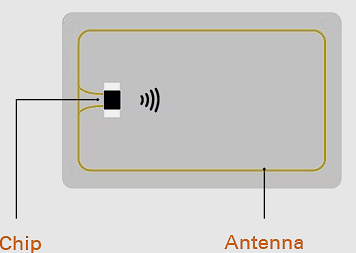
\includegraphics[width=0.4\textwidth]{images/research/emv_card}
    \caption{\centering Структура бесконтактной EMV-карты}
    \label{fig:emv_card}
\end{figure}

С распространением технологии NFC появилась сфера мобильных платежей.
Покупатели получили возможность быстро и безопасно выполнять оплату посредством устройств с поддержкой NFC с помощью виртуальных карт, добавленных в приложение «цифрового кошелька».
Примеры подобных приложений: Apple Pay, Google Pay, Mir Pay и др..



\subsection{Анализ процесса платежа через терминал}
\label{subsec:payment_process}

\subsubsection{Оплата бесконтактной картой}
\label{subsubsec:contactless_payment}

Процесс оплаты с использованием бесконтактной банковской карты может протекать несколькими различными способами.
Как уже было упомянуто ранее, есть онлайн и офлайн оплата через терминал.
Первая происходит с запросом подтверждения банком-эквайера от банка-эмитента в реальном времени.
Вторая происходит исключительно без моментального подтверждения банком, с участием карты и платежного терминала, который проводит ее аутентификацию.
Также для оплаты могут использоваться разные типы карт.
Однако именно бесконтактную оплату поддерживается только картами, соответствующими стандарту EMV.

При этом карта в защищенной области памяти хранит общий с эмитентом ключ MK-AC (Application Cryptogram Master Key).
Во время совершения оплаты при онлайн-операции карта генерирует на основе MK-AC сессионный ключ SK-AC (Application Cryptogram Session Key) и использует его, данные карты и данные об операции, полученные с терминала, для генерации криптограммы операции ARQC (Authorization Request Cryptogram).
В основе генерации криптограммы лежит алгоритм 3DES (Triple DES).
В общем случае данные по операции поступают от карты к платежному терминалу, далее на хост банка-эквайера, затем к платежной системе и на самом последнем этапе к банку-эмитенту для авторизации.
Результат авторизации передается назад на платежный терминал и карту.
Данный процесс изображен на рисунке~\ref{fig:emv_card_payment}.

\begin{figure}[H]
    \centering
    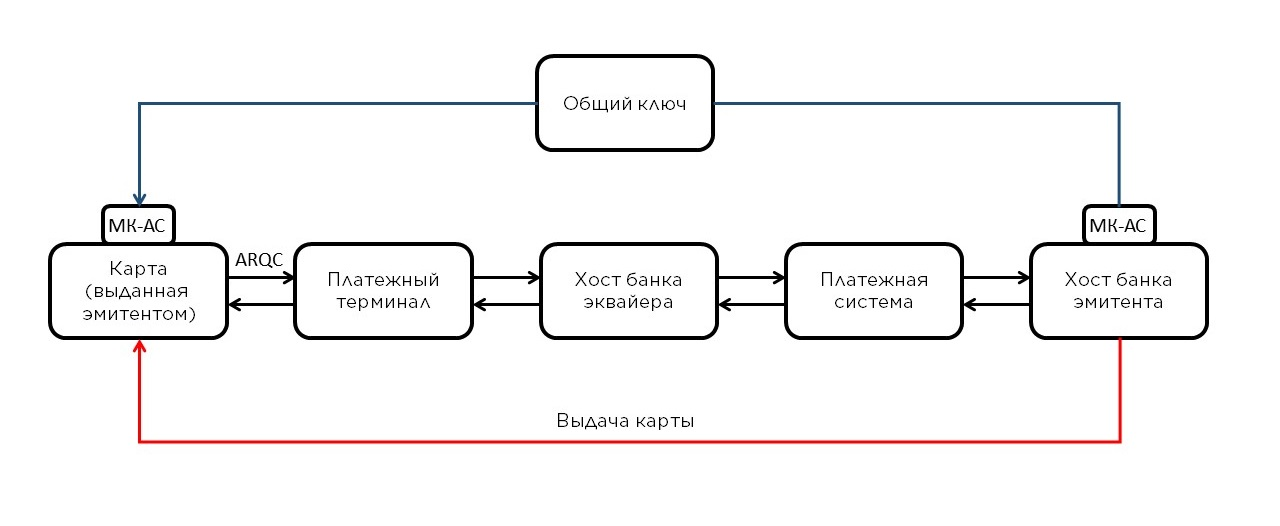
\includegraphics[width=0.8\textwidth]{images/research/emv_card_payment}
    \caption{\centering Процесс оплаты посредством EMV-карты}
    \label{fig:emv_card_payment}
\end{figure}

Банк-эмитент проверяет пришедшую криптограмму операции, путем ее сравнения со значением, которое генерирует сам на основе данных об операции, пришедших вместе с ARQC.
Банк-эмитент может одобрить или отклонить операцию по результатам анализа данных карты, криптограммы, установленных лимитов операций, рисков, а также других параметров~\cite{habr_nspk_mir_payment}.

Далее банк-эмитент на основе динамических данных транзакции генерирует ARPC (Authorisation Response Cryptogram) и отправляет эту криптограмму карте.
В тот момент, когда карта подтвердит пришедший ARPC, взаимная аутентификация карты и эмитента – выполнена~\cite{emv_card_mechanism}.


\subsubsection{Оплата мобильным приложением-кошельком}

При оплате мобильным кошельком выданная банком-эмитентом карта непосредственного участия в оплате не принимает.
Держатель карты вносит данные карты в цифровой кошелек, после чего карта «добавляется» в приложение, точнее не она, а специальный токен-профайл, сгенерированный на базе этой карты.
При этом карточные данные и ключ эмитента MK-AC, хранимый на карте, на телефон не передаются, поэтому оплата посредством приложения происходит с использованием токен-профайла и его специальных ключей.

Процесс добавления карты в приложение-кошелек представлен на рисунке~\ref{fig:add_mob_cardholder}.

\begin{figure}[H]
    \centering
    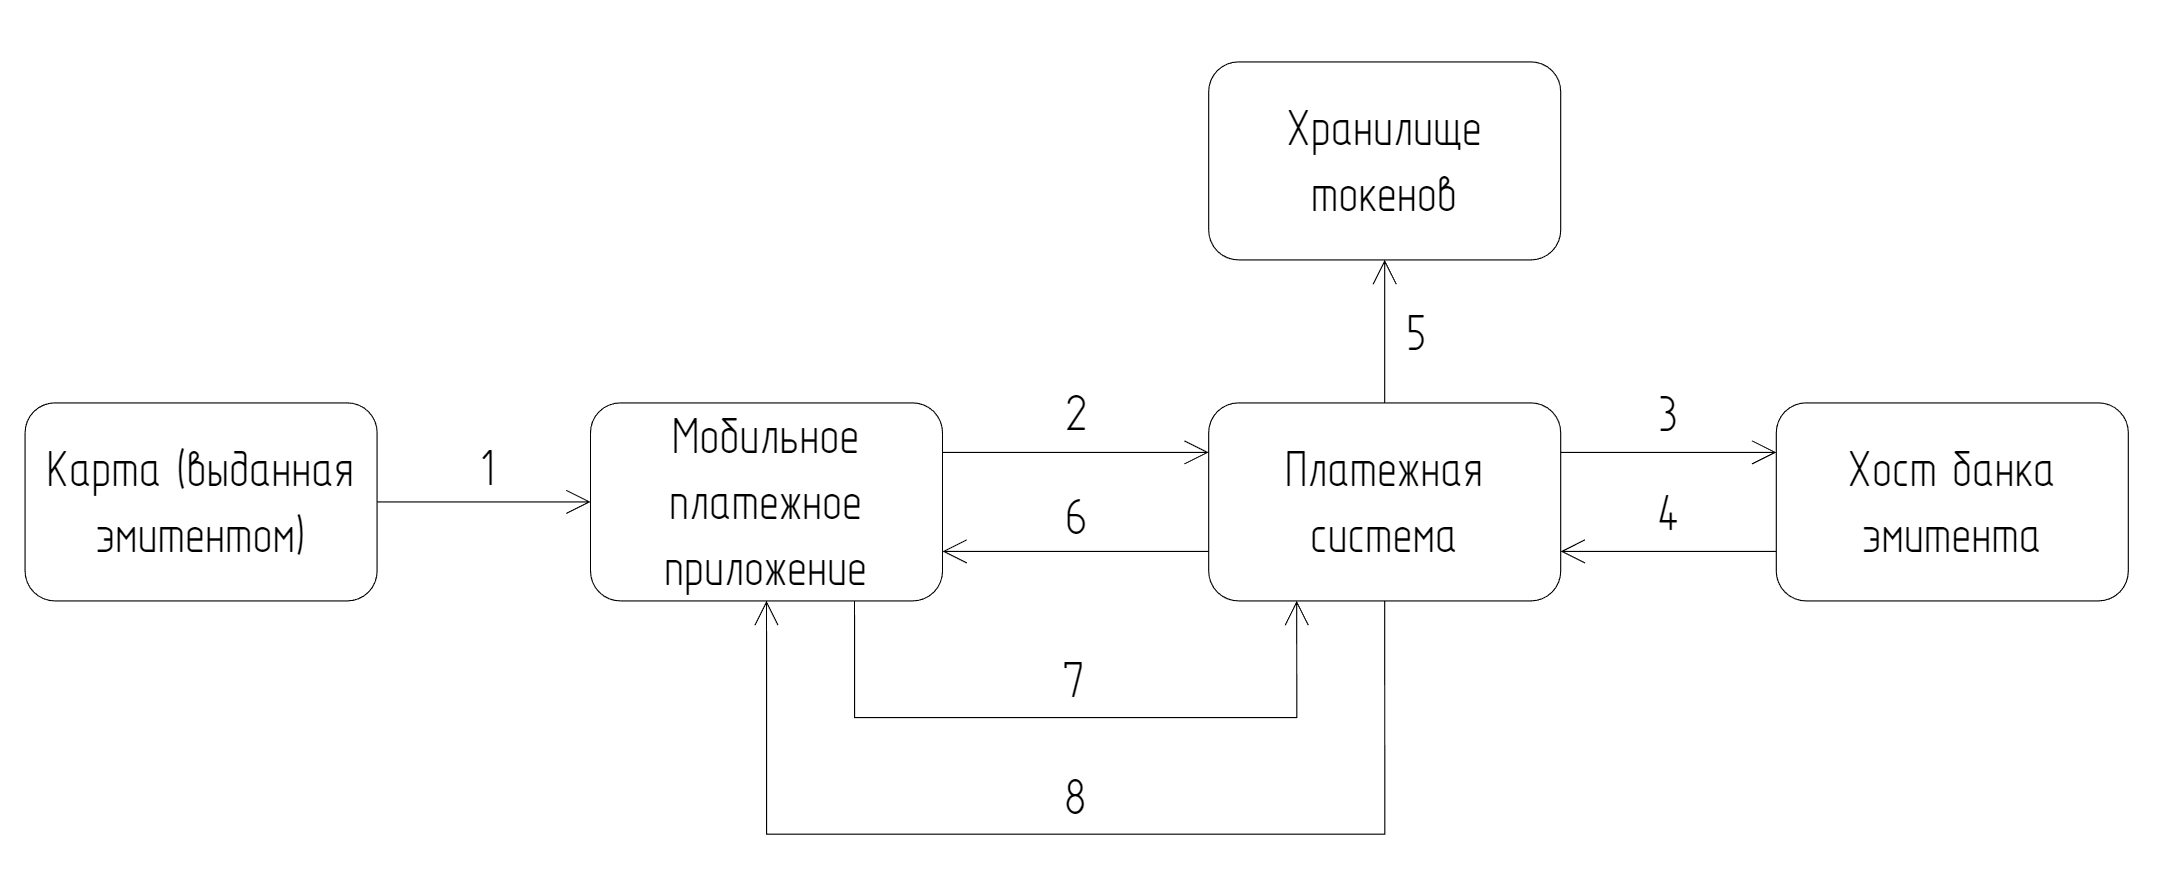
\includegraphics[width=0.8\textwidth]{images/research/add_mob_cardholder}
    \caption{\centering Процесс оплаты посредством мобильного приложения-кошелька}
    \label{fig:add_mob_cardholder}
\end{figure}

Цифрами на рисунке~\ref{fig:add_mob_cardholder} обозначены следующие этапы добавления карты в кошелек:

\begin{enumerate}
    \item держатель карты вводит данные в приложение;
    \item приложение передает их в зашифрованном виде через поставщика услуг мобильного кошелька(WSP~-- Wallet Service Provider) в платежную систему (в случае приложения Mir Pay поставщиком услуг кошелька является НСПК~-- Национальная система платежных карт~-- поэтому данные сразу попадают в ПС);
    \item платформа мобильных платежей (ПМП) производит обработку данных: расшифровывает их, по номеру карты определяет, каким эмитентом она была выдана, и запрашивает у него подтверждение на возможность добавления карты в кошелек;
    \item банк-эмитент возвращает подтверждение или запрет на возможность добавления карты в кошелек;
    \item в случае получения подтверждения для данной карты происходит процедура генерации токен-профайла;
    \item передачи токен-профайла в мобильное приложение пользователя;
    \item мобильное приложение запрашивает у ПМП несколько одноразовых ключей, которые будут использоваться приложением при совершении покупки в качестве сессионных ключей для проведения операции, аналогичных SK-AC.
\end{enumerate}

Таким образом, вместо карточных данных на мобильном устройстве будет храниться токен-профайл, который привязан к конкретным карте и устройству.
Преобразование токен-профайла в исходные данные карты вне платформы мобильных платежей является невозможным.
Одноразовые ключи не могут быть применены более одного раза, поэтому в процессе использования мобильное приложение с некоторой периодичностью подгружает из ПМП новые ключи.


Стоит отметить, что в Mir Pay используется схема, при которой происходит хранение нескольких одноразовых ключей, но существует и другой подход, при котором происходит хранение одного ключа на устройстве.
Такой подход требует наличия аппаратного элементов безопасности (АЭБ) на устройстве, например TEE (Trusted Execution Environment) или SE (Secure Element), и некоторые кошельки применяют именного этот подход, однако он накладывает ограничение в виде наличия АЭБ в устройстве.
Mir Pay также использует АЭБ при его наличии, но уже для хранения одноразовых ключей.

Высокая степень безопасности при использовании приложения гарантируется тем, что для обмена конфиденциальными данными ПМП и Mir Pay генерируют ключевые пары и обмениваются лишь публичными компонентами.
При этом хранением разных ключевых компонент происходит в разных системных хранилищах: как в ключевом хранилище, так и в оперативной памяти.
Для совершения мошеннической операции придется извлечь и расшифровать криптограммы всех ключей, а это неэффективно, в силу того, что для проведения операций используются строго одноразовые ключи.
Передача конфиденциальных данных, например токен-профайла, одноразовых ключей для проведения операций и данных по уже совершенным операциям, начинается только после того, как Mir Pay и ПМП обменялись публичными ключами, создав защищенный канал, и происходит только с использованием <<крипто-стойких>> алгоритмов~\cite{habr_nspk_mir_payment}.

Процесс оплаты с помощью приложения кошелька представлен на рисунке~\ref{fig:emv_mob_payment}.

\begin{figure}[H]
    \centering
    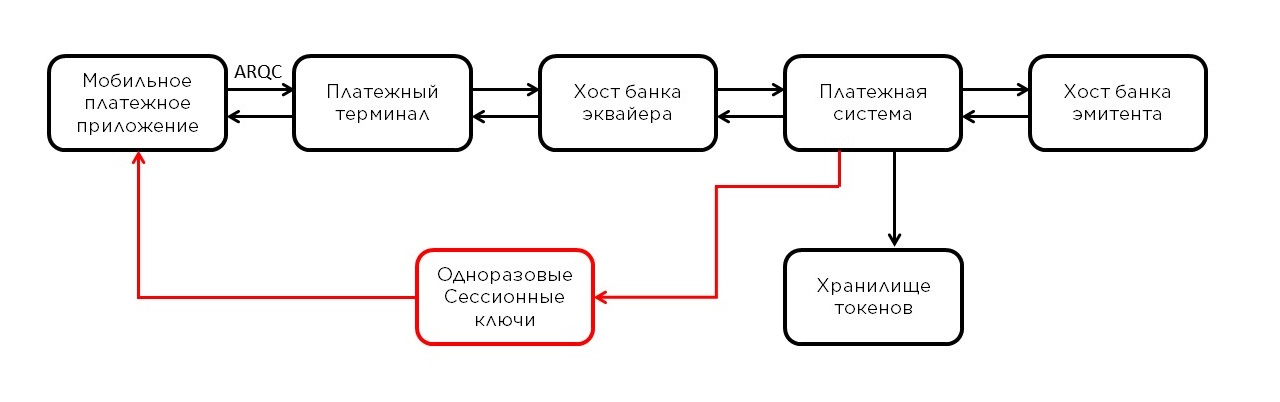
\includegraphics[width=0.8\textwidth]{images/research/emv_mob_payment}
    \caption{\centering Процесс оплаты посредством мобильного приложения-кошелька}
    \label{fig:emv_mob_payment}
\end{figure}

При оплате с помощью мобильного приложения-кошелька используются данные токен-профайла, а криптограмма ARQC генерируется на основе одного из одноразовых ключей (вместо SK-AC как при оплате картой).
Также при оплате приложением может использовать алгоритм шифрования, отличный от 3DES.
В частности в Mir Pay для генерации криптограммы используется более современный симметричный алгоритм блочного шифрования AES (Advanced Encryption Standard).

После генерации ARQC данные об операции так же, как и при оплате банковской картой, проходят через терминал и хост банка-эквайера, попадая в платежную систему.
По наличию токена и его номеру (из токен-профайла) платежная система определяет, что производится полата с помощью мобильного приложения, и направляет данные операции в ПМП для проверки криптограммы и детокенизации~-- превращения токена в данные соответствующей банковской карты.
Данные операции вместе с данными карты отправляются для авторизации в банк-эмитент.
После чего на основе ответа банка-эмитента запускается процесс обратного преобразования платежных данных.

Отличие от оплаты картой как раз в том, что криптограмма проверяется не эмитентом, а ПМП, так как одноразовые ключи и токен-профайл генерируются именно в в платформе мобильных платежей~\cite{habr_nspk_mir_payment}.



\subsection{Анализ существующих решений для оплаты}

\subsubsection{POS-терминалы}

Банковские платежи, в том числе бесконтактные, являются частью торгового эквайринга~--- сервиса офлайн оплаты товаров и услуг банковскими картами, предоставляемого предпринимателям различными банками.
POS-терминал (от англ.\ Point of Sale, точка продаж)~--- это устройство, предназначенное для приема безналичных платежей с использованием платежных средств, поддерживаемых терминалом.
POS-терминалы широко используются в розничной торговле, ресторанах, транспорте и других сферах, где требуется осуществление офлайн платежей.

Основные функции POS-терминалов:

\begin{itemize}
    \item инициация взаимодействия с платежным средством (карта, смартфон и прочее);
    \item обмен данными с платежным средством, получение данных для формирования транзакции;
    \item связь с банком (напрямую или с помощью устройства-хоста) для авторизации и выполнения транзакций;
    \item выдача чека потребителю (в печатном или электронном виде), возврат ошибки платежа;
    \item обеспечение безопасности платежа.
\end{itemize}

POS-терминалы имеют различную структуру, однако можно выделить обобщенную структуру данного устройства.
Она представлена на рисунке~\ref{fig:postrem_struct}.

\begin{figure}[H]
    \centering
    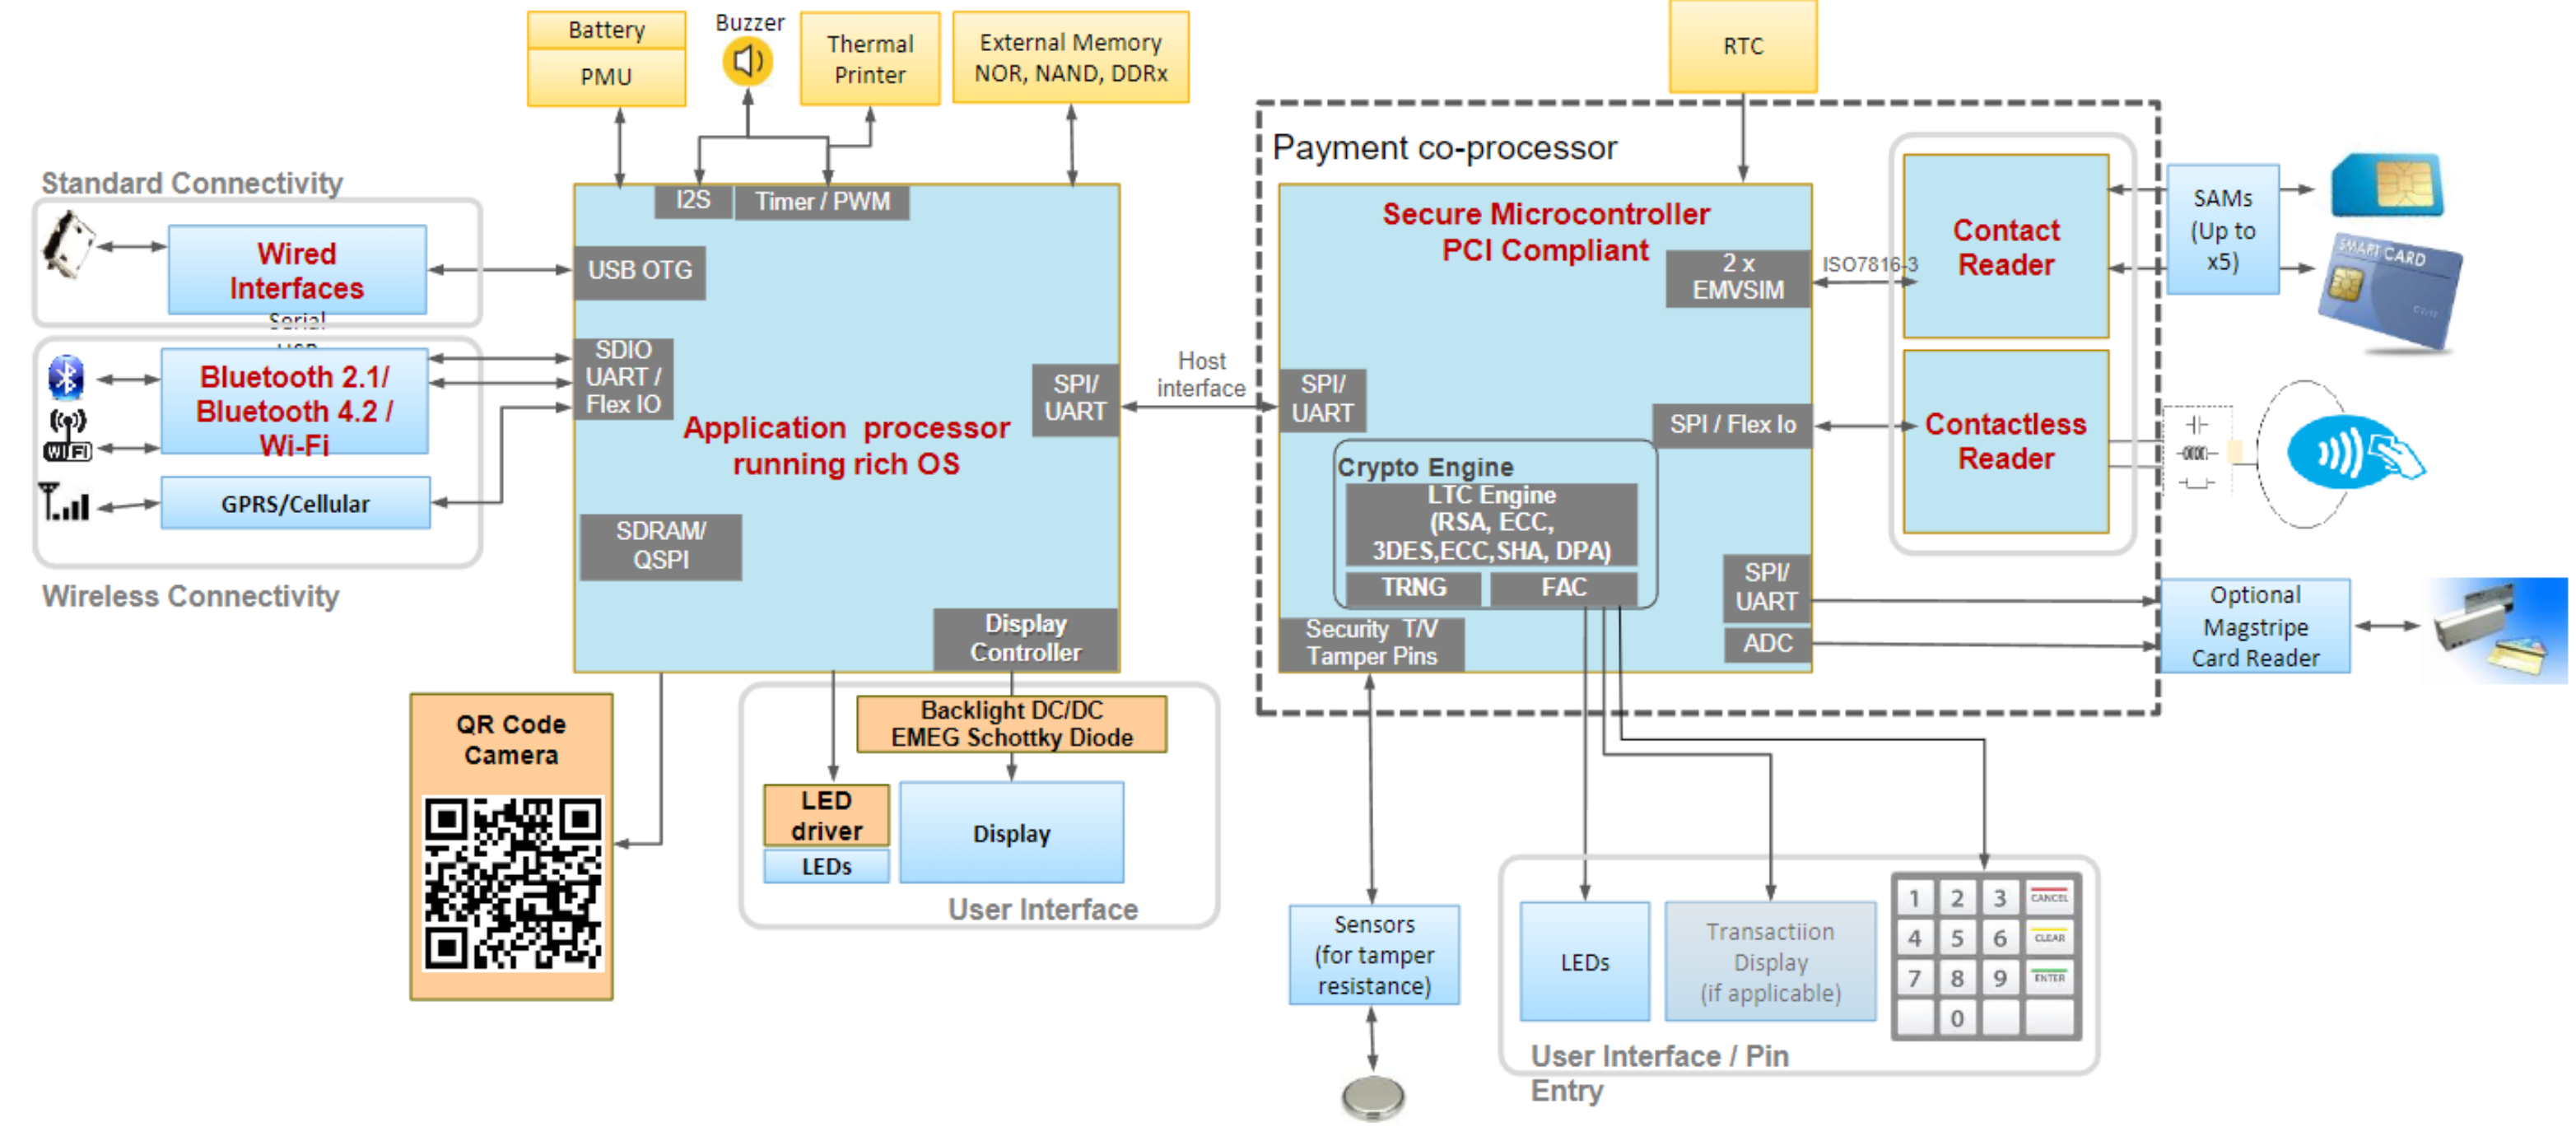
\includegraphics[width=1\textwidth]{images/research/postrem_struct}
    \caption{\centering Распространенная структура POS-терминала}
    \label{fig:postrem_struct}
\end{figure}

К обязательным элементам данного устройства можно отнести следующие:

\begin{itemize}
    \item RFID считыватель для обнаружения и связи со средствами платежа бесконтактным образом;
    \item модули проводной и/или беспроводной связи для связи с устройством-хостом или прямой связи с банком-эквайером.
\end{itemize}

Стоит отметить, что работа подобного устройства не возможна без программного обеспечения, интегрированного в POS-систему, которое управляет формированием и обработкой транзакций, шифрованием данных, запросами на авторизацию и связь с платежными сетями.

Одной из разновидностей торгового эквайринга является мобильный эквайринг, в нем в качестве платежного терминала используется mPOS- и softPOS-терминалы.

\begin{itemize}
    \item mPOS-терминал~--- это портативное устройство, состоящее из смартфона или планшета с подключенным внешним аппаратным модулем для работы с банковскими картами, которое используется для приема платежей;
    \item softPOS терминал~--- это программное решение, с помощью которого мобильное устройство с поддержкой NFC (как правило смартфон или планшет) выступает в роли платежного терминала, т.е. принимает бесконтактные средства платежа, используя встроенный модуль NFC, и осуществляет прием платежей~\cite{pos_term}.
\end{itemize}

Детальное сравнение разновидностей POS-терминалов приведено в таблице~\ref{tab:pos_comparison}.

\begin{table}[H]
    \caption{Сравнение POS, mPOS и SoftPOS терминалов}
    \label{tab:pos_comparison}
    \begin{sloppypar}
        \centering
        \begin{tabularx}{\textwidth}{ | >{\raggedright\arraybackslash}X | >{\raggedright\arraybackslash}X | >{\raggedright\arraybackslash}X | >{\raggedright\arraybackslash}X | }
            \hline
            \textbf{Особенность} & \textbf{POS-терминалы} & \textbf{mPOS-терминалы} & \textbf{SoftPOS-терминалы} \\
            \hline
            Требования к оборудованию & специальные аппаратные компоненты & мобильное устройство с выходом в сеть и Bluetooth и внешний считыватель карт & смартфон или планшет с поддержкой NFC \\
            \hline
            Мобильность & стационарные & мобильные & мобильные \\
            \hline
            Методы оплаты & любые виды платежей & любые виды платежей & бесконтактные платежи \\
            \hline
            Особенности настройки & необходимость интеграции с сетью и окружением & требуется установка приложения на мобильное устройство с выходом в сеть и подключение считывателя карт & только установка приложения на устройство с выходом в сеть \\
            \hline
            Пользовательский интерфейс & отдельный экран устройства & экран мобильного устройства и экран считывателя & экран мобильного устройства \\
            \hline
        \end{tabularx}
    \end{sloppypar}
\end{table}


\subsubsection{Сравнение существующих устройств}

На российском рынке услугу мобильного эквайринга предлагаются различными банками, а также специализированные поставщики оборудования.
Банки преимущественно предоставляют услуги эквайринга с использованием стационарные POS-систем, они имеют высокую привязку к месту установки, поэтому их применение в мобильном бизнесе (бизнес, предусматривающий продажу товаров и оказание услуг на выезде) ограничено.
Сбербанк предоставляет услуги мобильного эквайринга на базе mPOS-терминалов фирмы Эвотор, которые выступают не только в качестве платежного устройства, но и в качестве фискального накопителя для осуществления учета товара~\cite{sber_acq}.

Специализированные поставщики оборудования, такие как 2can осуществляют производство mPOS-терминалов, ПО для них, а также разработку собственного softPOS-решения.
Они осуществляют партнерское взаимодействие с банками, предоставляя услуги эквайринга по фиксированной стоимости, и за фиксированный процент со всех успешно проведенных платежных операций~\cite{2can_mpos}.
А также реализуют совместимость терминала с платежными приложениями других компаний, например <<1C: Мобильная касса>> посредством разработки и поддержки интеграционного приложения, а также использования актуальных аппаратных решений (терминалов), сертифицированных регулирующими органами.

Сравнением технологических характеристик распространенных mpos-терминалов представлено в таблице~\ref{tab:mpos_comparison}.
% устройства первоначально были взяты с https://v8.1c.ru/1s-kassa/mobilnoe-prilozhenie-1s-mobilnaya-kassa/   `1С:Мобильную кассу на смартфоне`

\begin{table}[H]
    \caption{Сравнение характеристик mPOS-терминалов}
    \label{tab:mpos_comparison}
    \begin{sloppypar}
        \centering
        \begin{tabularx}{\textwidth}{ | >{\raggedright\arraybackslash}X | >{\centering\arraybackslash}X | >{\centering\arraybackslash}X | >{\centering\arraybackslash}X | >{\centering\arraybackslash}X | >{\centering\arraybackslash}X | }
            \hline
            \textbf{Характе\-ристика} & \textbf{PAX D230} & \textbf{Verifone VX675} & \textbf{Aisino VM30} & \textbf{Ingenico iPP320} & \textbf{2can P17} \\
            \hline
            Поддержка Wi-Fi & Да & Нет & Да & Нет & Нет \\
            \hline
            Поддержка GPRS/3G & Да & Да & Да & Нет & Нет \\
            \hline
            Версия сертификата PCI PTS & 6.x & 3.0 & 5.x & 3.x & 3.1 \\
            \hline
            Интеграция~с платежным сервисом & зависит от банка & зависит от банка & зависит от банка & зависит от банка & SDK и REST API \\
            \hline
            Стоимость (мин.), тыс.\ рублей & 23 & 11 & 9 & 19 & 8 \\
            \hline
        \end{tabularx}
    \end{sloppypar}
\end{table}

% Verifone VX675 - https://techplat.ru/pos---terminal-verifone-vx-675-wi-fibtctls/  https://mirbeznala.ru/product/verifone-vx675-gprs-ctls-b-u/
% Aisino VM30 - https://cnvanstone.en.made-in-china.com/product/NJBrmIbTbFcD/China-Cheapest-Contactless-Card-Payment-Machine-Vm30-Mpos-Card-Reader.html  (цена)https://mirbeznala.ru/product/mpos-terminal-aisino-vm30/?srsltid=AfmBOorvKHSmqTDupSOvhsfPhqaJosEoSJpBhtb5Py6Hxlca2d3oy_uJ
% Ingenico iPP320 - https://mirbeznala.ru/product/ingenico-ipp-320-novyy/?srsltid=AfmBOooqXx7twi2Wg_25vM7lI9phsazEMrYhy-tb49VgRkWvph4EDY-m#char
% 2can P17 - https://1c.ru/news/info.jsp?id=23121
% убрал из сравнения: PAX D210E - https://mirbeznala.ru/product/perenosnoy-terminal-pax-d210e/

Все устройства подключаются к мобильному устройству по Bluetooth (версии различаются, но их различия оказывают незначительное влияние на работу) поддерживают бесконтактную оплату и сертифицированы по стандартам EMV L1\&L2 и EMV Contactless L1, посредством интеграции с внешним ПО поддерживают интеграцию с ОФД (операторами фискальных данных), т.е. системой учета товаров.

Продолжением развития мобильных терминалов можно считать смарт-терминалы~--- программно-аппаратные устройства состоящие из устройства на базе высокоуровневой ОС, например, Android и считывателя платежных карт.
Структура такая же как у mPOS-терминала, однако устройства находятся в едином корпусе и для их подключения используется проводной метод.

Сертификация EMV Level 1 подтверждает соответствие считывателя карты требованиям стандарта EMV по электрическим, механическим и функциональным параметрам.

Сертификация EMV Level 2 подтверждает соответствие программного обеспечения, реализующего обработку платежных транзакций стандарту EMV в части функциональных тестов по выполнению основных функций обработки транзакций;

PCI PTS (Payment Terminal Security)~--- это стандарт безопасности, разработанный PCI Security Standards Council, который устанавливает требования к защите аппаратных устройств, используемых для обработки данных карты (POS-терминалов, mPOS, ATM и т.д.).
Этот стандарт призван обеспечить высокий уровень защиты от несанкционированного доступа к конфиденциальной информации: данным магнитной полосы, номеру карты, PIN-коду, ключам шифрования и другим данным.


\subsection{Анализ платежных технологий}

В подразделе~\ref{subsec:payment_process} были рассмотрены стандартные сценарии выполнения платежных операций.
В рамках разработки системы отдельного внимания заслуживают процессы взаимодействия платежного терминала с банковской картой (или мобильным платежным приложением) и с хостом банка-эквайера.
Анализа данных процессов и используемых в них технологий позволит обеспечить корректность работы разрабатываемой системы.

Наиболее важным в данном контексте является стандарт EMV, т.к. он описывает характеристики банковских карт и других средств бесконтактной оплаты, а также весь процесс формирования платежа.
ФСБ РФ совместно с ЦБ РФ определяют классификацию платежных устройств и устанавливают для них ряд функциональных требований на основе стандарта EMV~\cite{cbr_requirements}.

Требования к считывателю смарт-карт и протоколу взаимодействия с ними описаны в 4 книгах <<EMV Integrated Circuit Card Specifications for Payment Systems>>, которые затрагивают следующие аспекты:
\begin{itemize}
    \item книга 1 описывает требования интерфейса платежного терминала для взаимодействия со смарт-картой независимо от используемого платежного приложения;
    \item книга 2 описывает аспекты безопасности и хранения ключей доступа на платежных картах и терминалах для обеспечения их корректной работы и взаимодействия, а также дополнительные требования и рекомендации в отношении онлайн-связи между картой и эмитентом, управления
    криптографическими ключами на уровне терминала, эмитента и платежной системы.;
    \item книга 3 определяет процедуры взаимодействия терминала и платежной карты, необходимые для осуществления транзакции платежной системы;
    \item книга 4 определяет обязательные, рекомендуемые и необязательные требования к терминалу, необходимые для поддержки приема карт.
\end{itemize}

Требования для считывателя бесконтактных карт определены в <<EMV Level 1 Specifications for Payment Systems, EMV Contactless Interface Specification>>, а требования к протоколу обмена между считывателем и бесконтактной картой описаны в книгах <<EMV Contactless Specifications for Payment Systems>>:
\begin{itemize}
    \item книга A описывает архитектуру POS-терминала бесконтактной оплаты и общие требования к нему;
    \item книга B определяет спецификацию работы Entry Point~--- ПО, отвечающего за взаимодействие терминала и бесконтактной картой: выбор платежного приложения, активацию платежного ядра и использование его результатов;
    \item книги C (2-8) содержат описание принципов работы платежных ядер различных ПС.
\end{itemize}

Также для бесконтактных карт есть книга E, которая выступает в качестве аналога книге 2 из серии <<EMV Integrated Circuit Card Specifications for Payment Systems>>, также фокусируюсь на вопросах безопасности и хранения и использования ключей доступа, но уже на бесконтактных платежных картах.

\subsubsection{Стандарт EMV}

EMV~--- стандарт для банковских карт, совместно разработанный платежными системами Europay, Mastercard и Visa.
Он используется  международными платежными системами (МПС) для проведения операций по банковским картам.

Повышенный уровень безопасности карт стандарта EMV обусловлен наличием встроенного чипа, который называется Secure Element.
Чип хранит данные в зашифрованном формате, а также может запускать приложения на карте и обмениваться командами с кассовыми терминалами.

Банковская карта с поддержкой стандарта EMV, является стандартной смарт-картой, однако, имеет расширенный функционал.
Технология функционирования платежной карты (как контактной, так и бесконтактной) и взаимодействия платежного терминала с ней описана в стандарте ISO/IEC 7816 и в <<EMV Integrated Circuit Card Specifications for Payment Systems>>.
Технология работы с бесконтактной картой описана в стандарте ISO/IEC 14443, а также в <<EMV Contactless Specifications for Payment Systems>>.
Карта имеет операционную систему со встроенной файловой системой и приложениями, причем предназначенными не только для реализации платежей~\cite{emv_specifications_book}.

\paragraph{EMV-карта}

Главное новшество EMV-карт~--- возможность проверки динамической криптограммы карты (цифровой подписи ее статических данных).
Для карт с магнитной полосой терминалы не имели такую возможность и выполняли проверку только статических данных карты, в результате чего такие карты легко копировались.
Процесс аутентификации карты с магнитной полосой и EMV-карты представлен на рисунках~\ref{fig:magnetic_card_auth} и~\ref{fig:emv_card_auth} соответственно.

\begin{figure}[H]
    \centering
    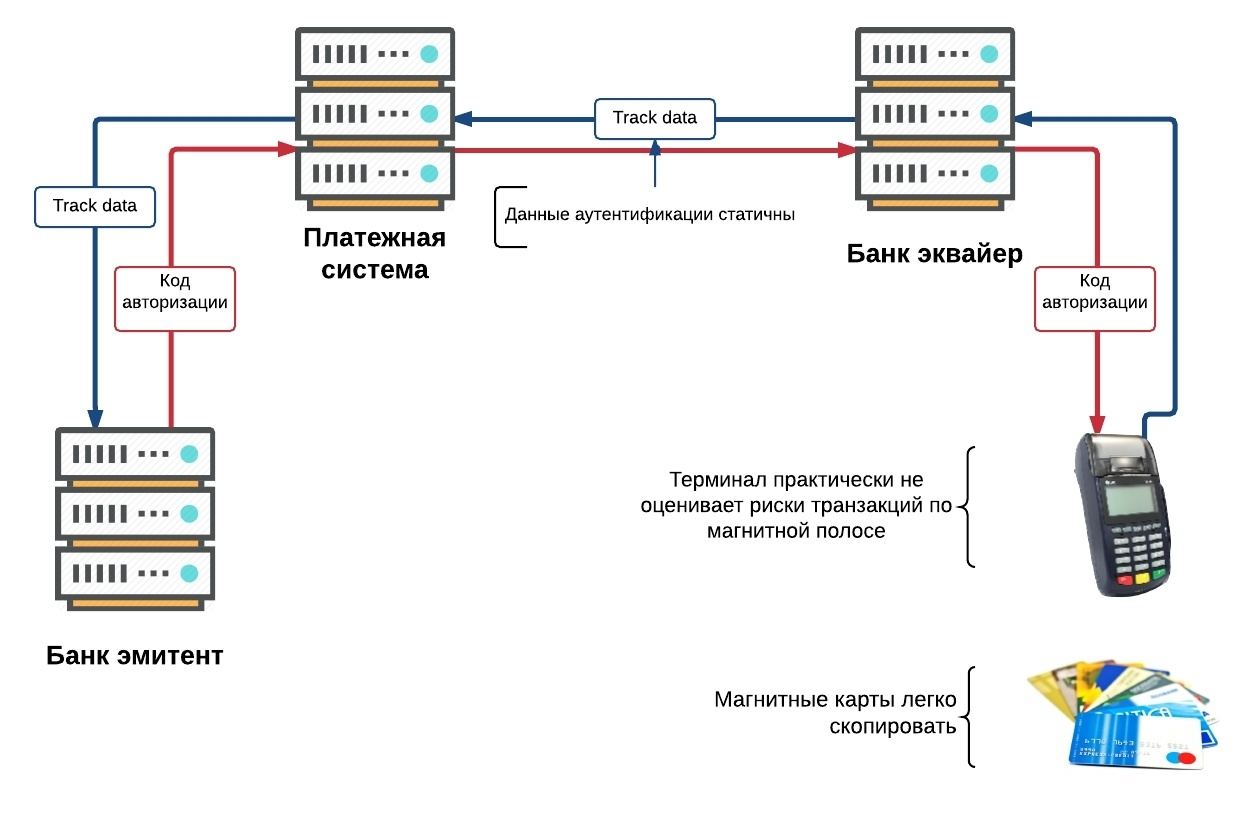
\includegraphics[width=0.8\textwidth]{images/research/magnetic_card_auth}
    \caption{\centering Аутентификации карты с магнитной полосой в ходе платежной транзакции}
    \label{fig:magnetic_card_auth}
\end{figure}

\begin{figure}[H]
    \centering
    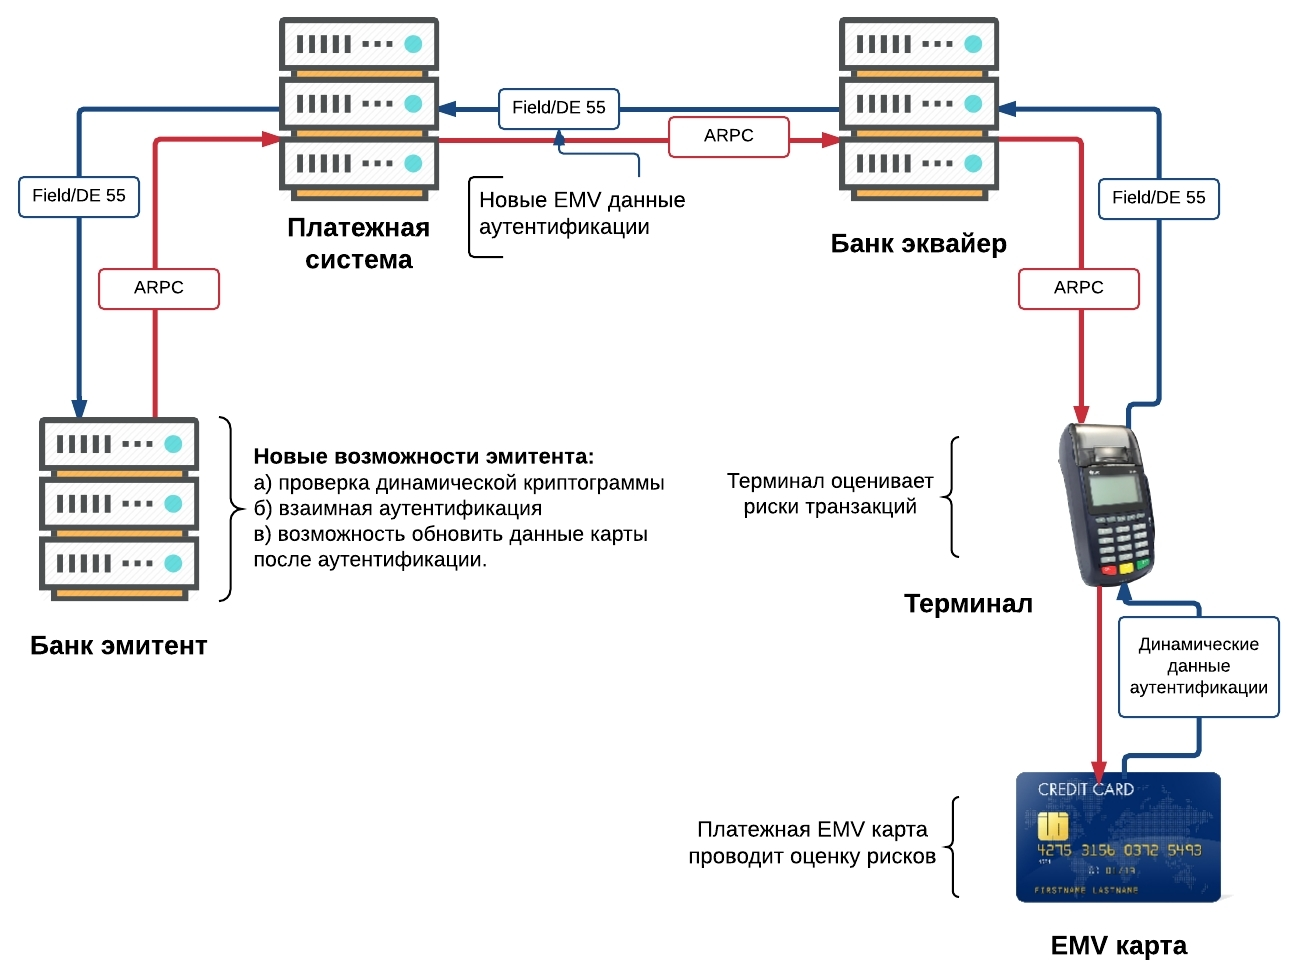
\includegraphics[width=0.8\textwidth]{images/research/emv_card_auth}
    \caption{\centering Аутентификации EMV-карты на основе динамической криптограммы в ходе платежной транзакции}
    \label{fig:emv_card_auth}
\end{figure}

Динамическая аутентификация карты в ходе EMV-транзакции происходит по следующему алгоритму:

\begin{enumerate}
    \item терминал передает данных о транзакции на карту (сумма, валюта, страна и пр.);
    \item происходит проверки рисков транзакции как картой, так и терминалом;
    \item если проверка не пройдена на карте, то процесс прерывается, если пройдена~-- карта подписывает данные транзакции;
    \item терминал помечает полученными от карты данные тегом <<DE 55>> (стандарт ISO 8583) и отправляет вместе с прочими в банк-эквайер;
    \item банк-эмитент выполняет проверку динамической подписи транзакции.
\end{enumerate}

Данные в Field/DE 55 содержится важная информация для оценки рисков транзакции  эмитентом и ПС, в частности Terminal Verification Result и Card Verification Result~\cite{emv_card_mechanism}.

Банк-эмитент также может выслать свою криптограмму карте для дополнительной аутентификации или обновить данные карты (например, лимит карты), записанные на чипе карты (уже после успешной аутентификации)~\cite{emv_book_2}.
Более подробно процесс формирования и проверки криптограммы уже был описан в пункте~\ref{subsubsec:contactless_payment}.

\paragraph{Платежные EMV-приложения}

Платежное EMV-приложение выступает в качестве интерфейса для взаимодействия с картой.
С помощью серии команд, поданных в приложение на карте осуществляется управление приложением и состоянием транзакции.

Для работы с приложениями на карте используются APDU-команды, описанные в стандарте ISO/IEC 7816--4, рассматриваемым в пункте~\ref{subsubsec:7816}.
С их помощью реализуется функционал приложения, например, создание банковской транзакции и управление ее состоянием.
Стоит также отметить, что производители карты реализуют свои собственные приложения для оплаты, реализуя при этом стандарт выполнения платежа в EMV, который называется EMV Transaction Flow, о нем речь пойдет в подпункте~\ref{par:emv_transaction}.

Каждое приложение имеет свой собственный идентификатор~--- AID (Application Identifier).
Он указывает к какому типу ПС относится приложение и для каких карт может использоваться (для карт одной ПС, могут использоваться разные приложения).
На основе идентификатора приложения AID терминал определяет возможность проведения транзакции или, в случае нескольких приложений, составляет список поддерживаемых приложений и предлагает выбрать одно из них для выполнение транзакции~\cite{emv_card_mechanism}.

\paragraph{Безопасность EMV-карты}

Любые смарт-карты, и EMV-карты не исключение, имеют механизм разграничения доступа, с помощью которого происходит контроль состояния карты в рамках текущей сессии подключения и механизм проверки условий доступа, другими словами, проверка прав на работу с файлами.
Наличие прав зависит от состояния карты в рамках текущей сессии, которое может изменяться вводом определенных предварительно заложенных кодов доступа~\cite{habr_smart_card_for_little}.

Также смарт-карты имеют встроенные механизмы для шифрования, однако их аппаратная реализация отличается в зависимости от производителя.
В EMV-чипах реализованы следующие алгоритмы шифрования:

\begin{itemize}
    \item RSA (асимметричное шифрование): применяется в EMV-картах для аутентификации и защиты данных, используется для динамической аутентификации (DDA) и комбинированной аутентификации (CDA), обеспечивая высокий уровень безопасности за счет генерации уникальных ключей для каждой транзакции;
    \item DES и 3DES (симметричное шифрование): DES - устаревший и менее безопасный стандарт, однако по-прежнему применяемый в некоторых системах, более распространенным является 3DES (Triple DES), который обеспечивает улучшенную безопасность за счет применения алгоритма DES трижды, эти алгоритмы используются для шифрования PIN-кодов;% TODO добавить ссылку на раздел про DES
    \item AES (Advanced Encryption Standard): современный симметричный алгоритм шифрования, предлагающий более высокий уровень безопасности по сравнению с DES и 3DES, благодаря более длинным ключам и более сложным методам шифрования, используется в технологии HCE (Host Card Emulation) для шифрования в приложениях <<Цифровых кошельках>> на мобильных устройствах;
    \item SHA-1 и SHA-256 (хэширование): используется для создания хэш-значений транзакций, из-за уязвимостей SHA-1 многие системы переходят на SHA-256, который обеспечивает более высокий уровень безопасности, с помощью хэш-функции гарантируется целостность данных в процессе транзакций~\cite{emv_fastercapital}.
\end{itemize}

Важно понимать, что персональная информация владельца карты в платежных приложениях не хранится, а сами приложения, ключи и некоторые PIN-коды, защищены от прямого доступа и модификации.
Однако, информация, не относящаяся к конфиденциальным данным, является доступной.
К подобной информации относятся различные данные, необходимые для выполнения платежных операций, в частности сертификаты ключей-доступа, номер карты (PAN), списки методов проверки карты (CVM~-- Card Verification Methods list) и другая информация.
Примерный перечень всех доступных для чтения данных приложения приведен на рисунке~\ref{fig:emv_available_data}.
Доступные данные организованы в записи (рекорды или треки), которые можно получить с помощью команд «Get Processing Options» и «Read Record», описанных  в ISO/IEC 7816.
Дополнительно данные технических настроек, таких как лимиты и счетчики, могут быть доступны через команду «Get Data» с указанием требуемого типа~\cite{emv_card_mechanism}.

\begin{figure}[H]
    \centering
    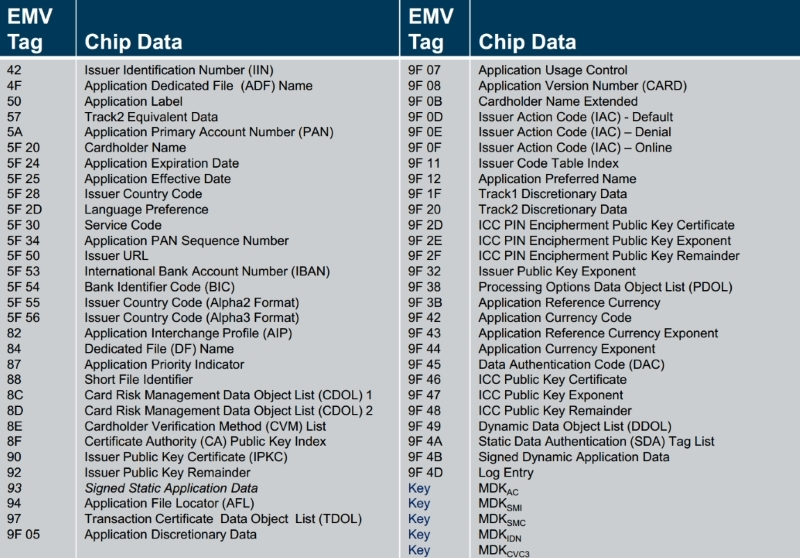
\includegraphics[width=0.8\textwidth]{images/research/emv_available_data}
    \caption{\centering Доступные данные платежного EMV-приложения}
    \label{fig:emv_available_data}
\end{figure}

Банковская платежная карта имеет несколько уровней защиты, определенных хронологией ее создания:

\begin{enumerate}
    \item производитель чипа карты задает некий первичный ключ для доступа к прошивке карты, с помощью него можно установить ОС;
    \item ОС карты также имеет свой ключ, который необходим для работы с файлами и приложениями на карте, с помощью него можно установить платежные приложения;
    \item платежные приложения на карте персонализируются с помощью определенных параметров и ключей приложения, заложенных банком-эмитентом с целью обеспечения безопасности EMV-транзакций.
\end{enumerate}

После чего, как правило, изменение работы карты и приложения становится практически невозможным без знания ключей.
Данные платежного приложения могут модифицироваться после выпуска карты посредством банкомата или терминала, которые после успешной аутентификации карты в ходе банковской транзакции, передает скриптовую командой, имеющую цифровую MAC-подписью, гарантирующей целостность данных.
Такая возможность предусмотрена для того, чтобы  банк-эмитент управлять блокировкой карты, обновлять лимиты или настройки.
В данном случае, MAC (Message Authentication Code)~--- это аналог цифровой подписи, который гарантирует целостность данных, переданных на карту.
Для его расчета используется соответствующий ключ приложения (один из 3-х DES ключей загружаемых в приложение).
% TODO добавить раздел про DES и ссылку на него

Технически возможно перенести данные с одной банковской карты на другую, если приложение на новой карте не персонализировано.
Однако отсутствие возможности доступа, а, как следствие, и копирования ключей делает карту неприменимой для проведения транзакций, т.к. без них приложение не сможет сгенерировать корректную подпись транзакции, что приведет к отклонению операции банком-эмитентом.
Кроме того, невозможность выполнить CDA (Combined Data Authentication) или DDA (Dynamic Data Authentication) существенно ограничивает использование копии.
Единственным уязвимым местом может быть SDA (Static Data Authentication), однако этот метод уже считается устаревшим и редко используется как единственный механизм аутентификации~\cite{emv_card_mechanism}.

\paragraph{EMV-транзакция}
\label{par:emv_transaction}

В пункте~\ref{subsubsec:contactless_payment} уже упоминалось о существовании 2-х типов платежный транзакций: онлайн и офлайн, а также в общих чертах было рассмотрено выполнение онлайн транзакции.
Есть также 2 способа аутентификации: офлайн или Static Data Authentication (SDA) и онлайн или Dynamic Data Authentication (DDA).
Онлайн аутентификация проводится при непосредственном участии эмитента.
Офлайн-аутентификация, в свою очередь, выполняется самим платежным терминалом.
Важно отметить, что при обработке онлайн-операции могут одновременно использоваться как онлайн, так и офлайн аутентификация, если карта и терминал поддерживают оба метода, такой вид аутентификации называется Combined Data Authentication (CDA).

Любая платежная транзакция в соответствии со стандартом EMV начинается с выбора платежного приложения на терминале.
После выбора приложения терминал и карта выполняют ряд функций, которые схематично представлены на рисунке~\ref{fig:transaction_flow_example} в порядке своего выполнения.
Для каждой функции есть условия и ограничения применения, которые детально описываются стандартом.
В соответствии с EMV стандартом терминал во время транзакции должен выполнять только те функции, которые поддерживаются конкретной платежной картой~\cite{emv_book_3}.


\begin{figure}[H]
    \centering
    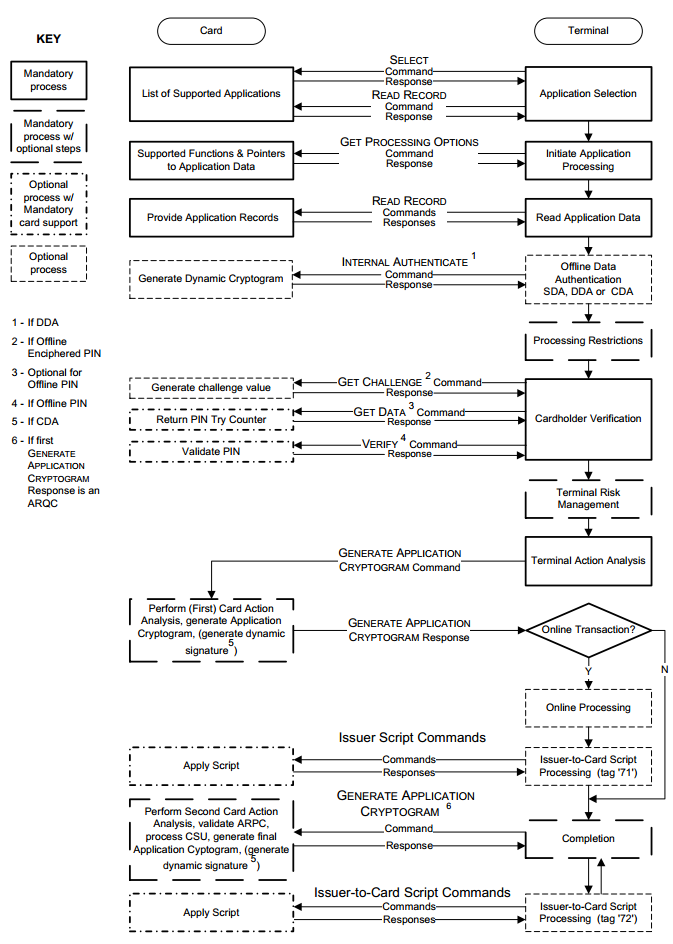
\includegraphics[width=0.8\textwidth]{images/research/transaction_flow_example}
    \caption{\centering Схема алгоритма выполнения транзакции терминалом}
    \label{fig:transaction_flow_example}
\end{figure}

За безопасность проведения транзакции отвечают следующие этапы:

\begin{itemize}
    \item аутентификация (офлайн, онлайн или комбинированная);
    \item оценка рисков проведения транзакции;
    \item верификация держателя карты на основе онлайн и/или офлайн PIN-кода, размера суммы транзакции, страны, валюты и прочих данных;
\end{itemize}

% TODO: заменить на корректное что-то, что меньше подпункта
\paragraphit{Онлайн аутентификация}

Процесс выполнения онлайн аутентификации представлен на рисунке~\ref{fig:online_auth}.
Его описание было приведено в пункте~\ref{subsubsec:contactless_payment}.

\begin{figure}[H]
    \centering
    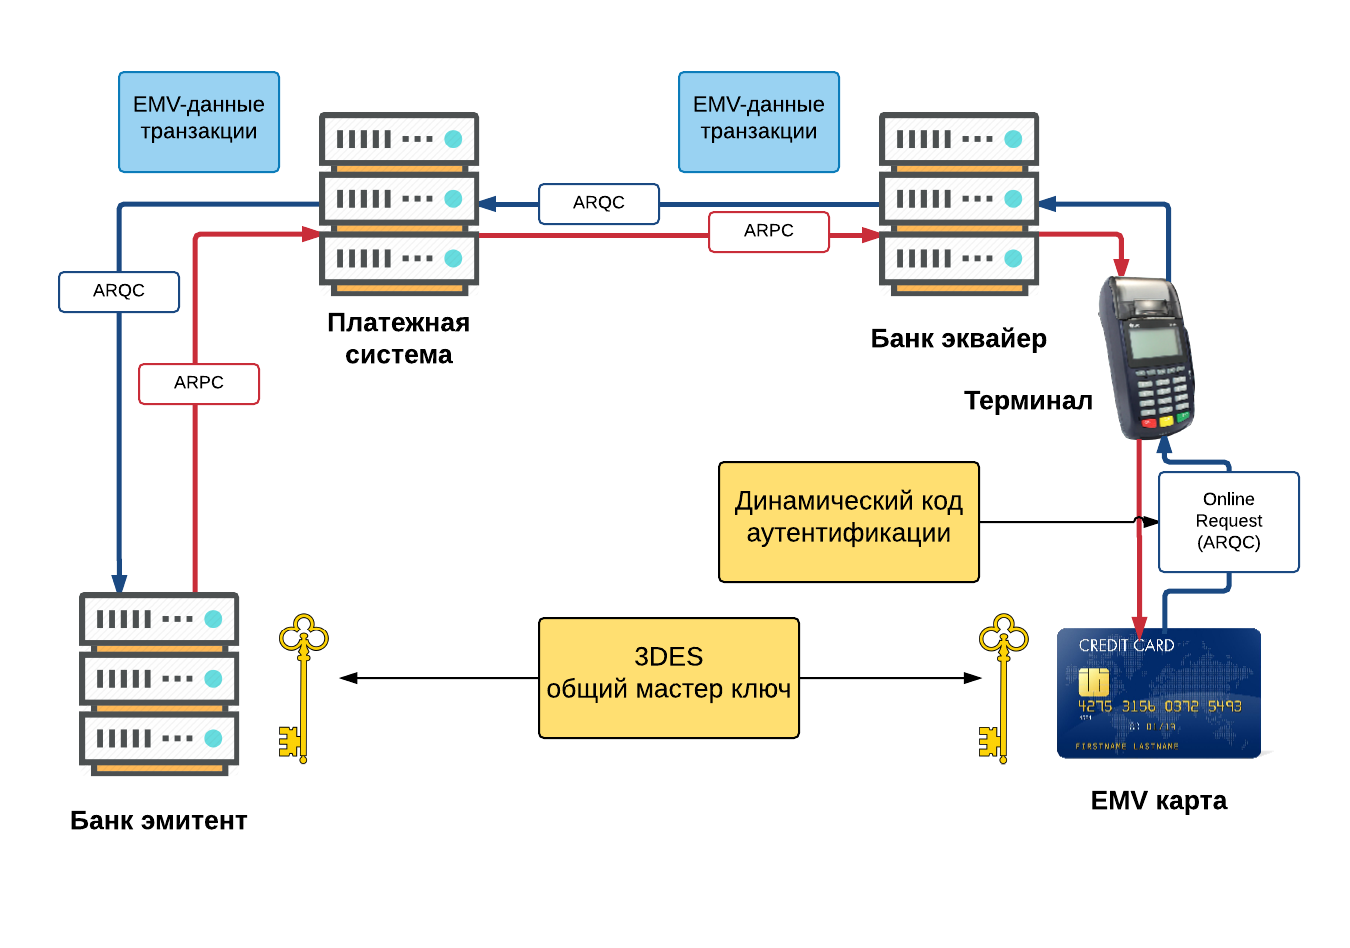
\includegraphics[width=0.8\textwidth]{images/research/online_auth}
    \caption{\centering Процесс выполнения онлайн аутентификации}
    \label{fig:online_auth}
\end{figure}


% TODO: заменить на корректное что-то, что меньше подпункта
\paragraphit{Офлайн аутентификация}

Как уже отмечалось ранее офлайн аутентификация происходит без непосредственного взаимодействия с банком или ПС в момент совершения операции.
Карта и терминал могут самостоятельно одобрить транзакцию, если её сумма не превышает установленный лимит.
Терминал же передает информацию в банк в соответствии с установленным режимом.
Преимущества данного подхода в том, что держатель карты может завершить оплату при отсутствии связи с банком, и операции на небольшие суммы выполняются значительно быстрее.

Офлайн аутентификация происходит с использованием асимметричной криптографии RSA.
Основная причина использования RSA заключается в распределении ключей: в онлайн-транзакциях ключи известны только карте и банку, тогда как в офлайн-процессе терминал также должен иметь доступ к ключу.
С учетом большого количества терминалов, повышается вероятность компрометации секретного ключа, что делает асимметричный подход более безопасным, т.к. терминал хранит только открытый ключ, а карта - секретный ключ.

Упрощенная модель статической аутентификации (Static Data Authentication) представлена на рисунке~\ref{fig:sda}.

\begin{figure}[H]
    \centering
    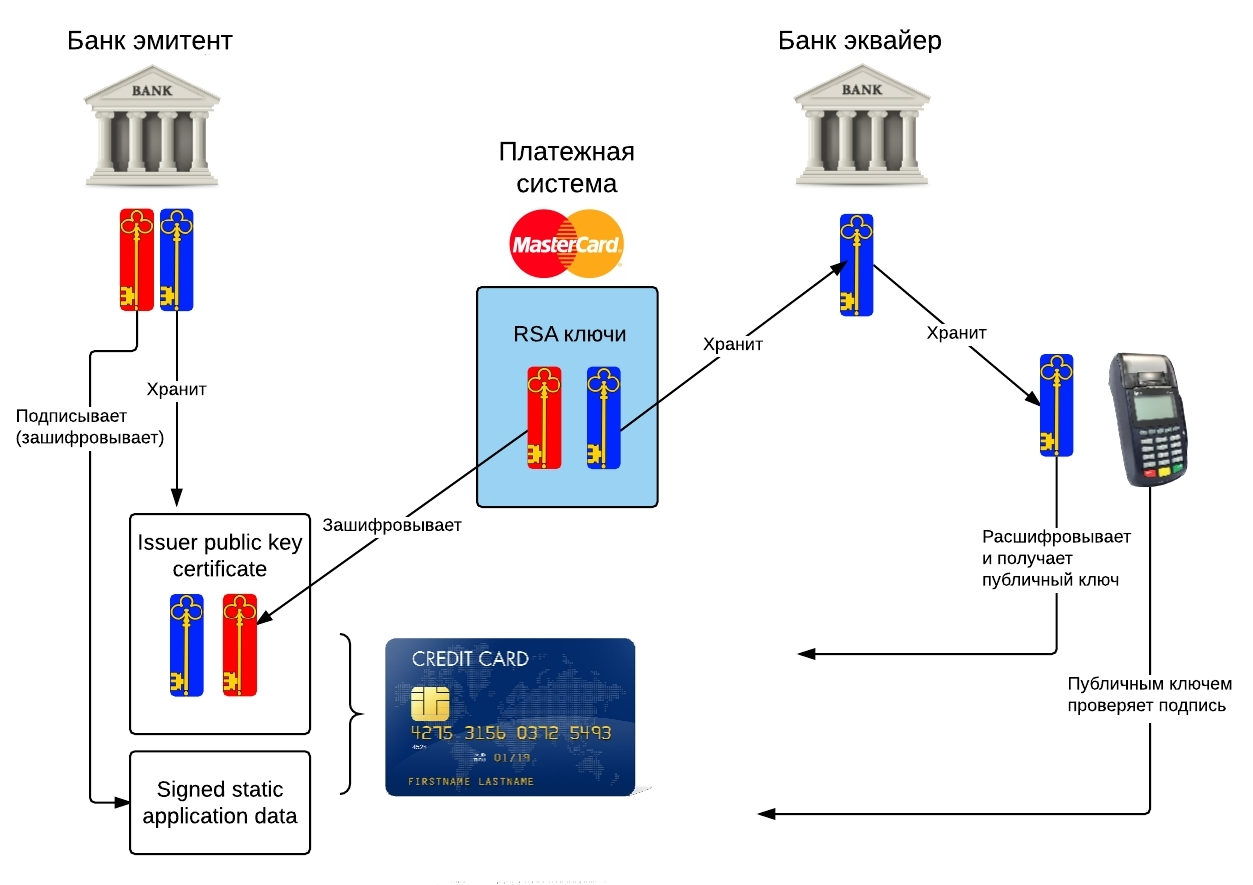
\includegraphics[width=0.8\textwidth]{images/research/sda}
    \caption{\centering Упрощенная модель Static Data Authentication (SDA)}
    \label{fig:sda}
\end{figure}

Центральную роль в этом процессе играет ПС, выступающая в качестве сертификационного центра, она создает пару ключей: секретный (красный) и открытый (синий).
Аналогичную пару ключей генерирует банк-эмитент.
Публичный ключ эмитента включается в специальный сертификат (Issuer Public Key Certificate), подписанный с использованием приватного ключа ПС.
Данный сертификат загружается на карту в процессе ее персонализации.

Когда платежный терминал подключается к торговой точке, в него загружается публичный ключ ПС через банк-эквайер.

Во время выполнения офлайн транзакции терминал осуществляет аутентификацию карты по следующему алгоритму:

\begin{enumerate}
    \item терминал считывает сертификат банка-эмитента (Issuer Public Key Certificate) с карты и с помощью публичного ключа ПС проверяет его подпись;
    \item если подпись сертификата подтверждена, терминал извлекает публичный ключ банка-эмитента из сертификата;
    \item данный ключ используется для проверки подписи критически важных данных карты, что позволяет удостовериться в её подлинности.
\end{enumerate}


% TODO: можно удалить абзац и картинку
Описание выполнение SDA из стандарта EMV приведено на рисунке~\ref{fig:emv_offline_sda}~\cite{emv_book_2}.

\begin{figure}[H]
    \centering
    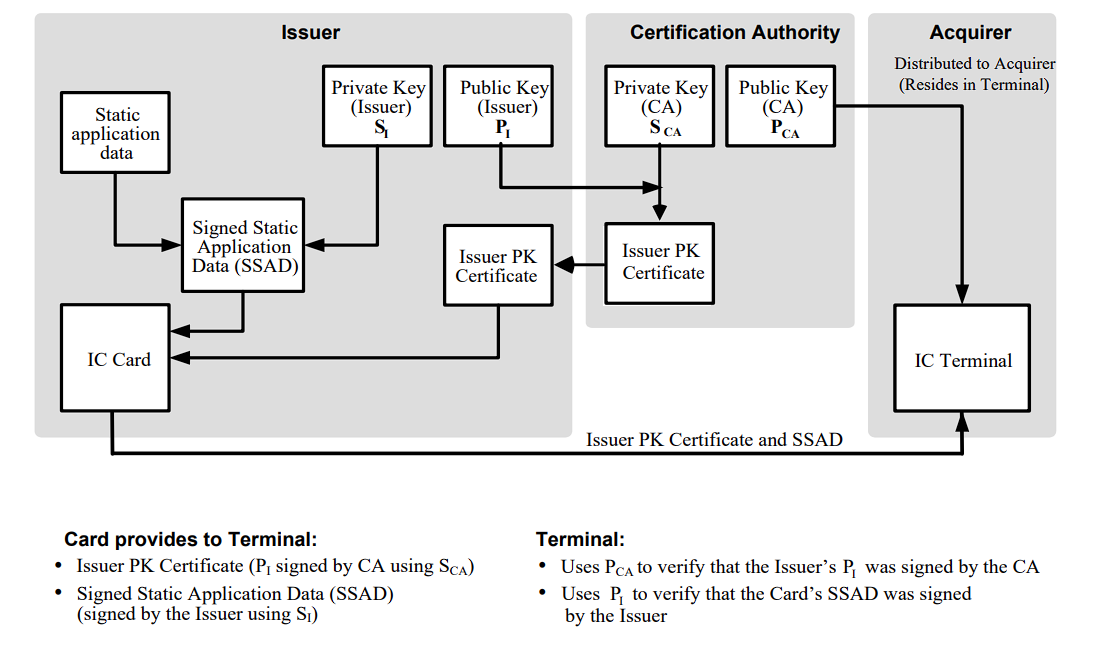
\includegraphics[width=0.8\textwidth]{images/research/emv_offline_sda}
    \caption{\centering Диаграмма Static Data Authentication (SDA)}
    \label{fig:emv_offline_sda}
\end{figure}

SDA в настоящее время уступает место более современным технологиям DDA (Dynamic Data Authentication) и CDA (Combined Data Authentication).
Эти методы включают в себя SDA, но также используют динамическое подписание данных, передаваемых между терминалом и картой.

Технология SDA позволяет удостовериться в неизменности данных на карте, но не обеспечивает полной защиты от копирования.
В отличие от неё, DDA и CDA подтверждают подлинность карты, поскольку карта хранит уникальный приватный ключ.
Сертификат этого ключа подписан приватным ключом эмитента, а сертификат эмитента~-- приватным ключом платежной системы.

DDA и CDA схожи по структуре: оба используют уникальный ключ карты и динамические данные.
Однако DDA выполняется как отдельная операция до начала основной транзакции, тогда как CDA интегрирована в транзакционный процесс и дополнительно подписывает криптограмму карты.
Несмотря на то, что CDA обеспечивает более высокий уровень безопасности, на практике чаще применяется DDA.

Описание выполнение офлайн DDA и CDA из стандарта EMV приведено на рисунке~\ref{fig:emv_offline_dda_cda}~\cite{emv_book_2}.

\begin{figure}[H]
    \centering
    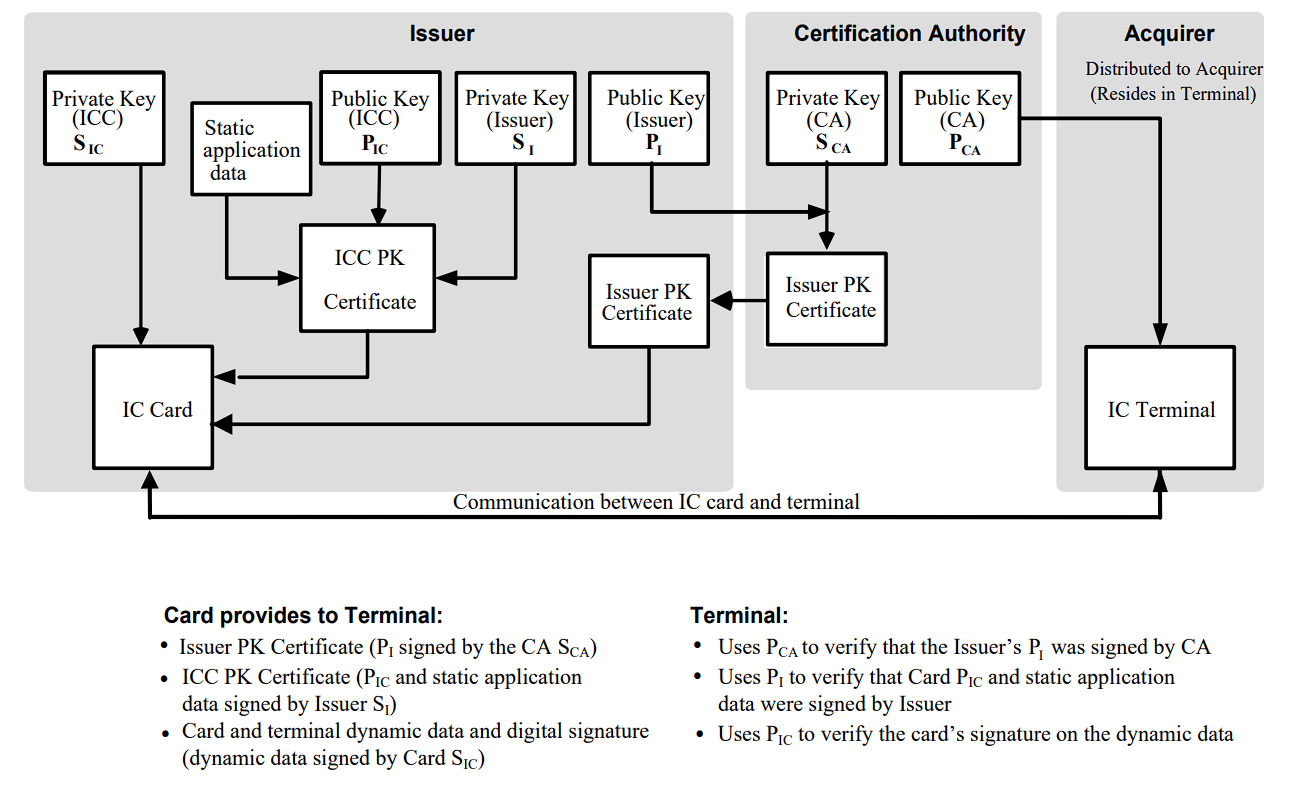
\includegraphics[width=0.8\textwidth]{images/research/emv_offline_dda_cda}
    \caption{\centering Диаграмма офлайн DDA и CDA}
    \label{fig:emv_offline_dda_cda}
\end{figure}

Также существует алгоритм офлайн DDA с использованием криптографии эллиптических кривых (Elliptic Curve Cryptography~-- ECC), который называется
Extended Data Authentication (XDA).

Описание выполнение офлайн XDA стандарта EMV приведено на рисунке~\ref{fig:emv_offline_xda}~\cite{emv_book_2}.

\begin{figure}[H]
    \centering
    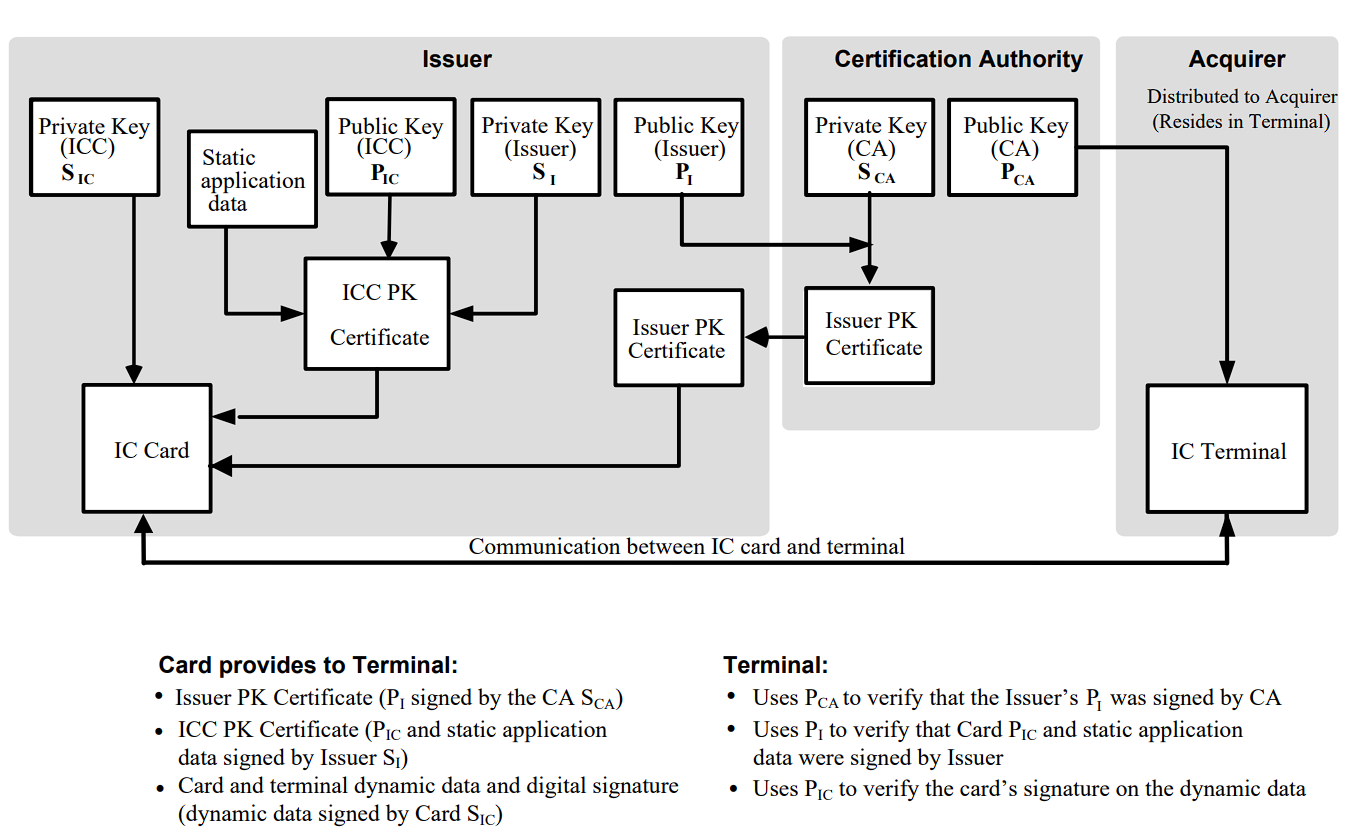
\includegraphics[width=0.8\textwidth]{images/research/emv_offline_xda}
    \caption{\centering Диаграмма офлайн XDA}
    \label{fig:emv_offline_xda}
\end{figure}


При выполнении XDA карта генерирует цифровую подпись, которая проверяется терминалом.
Эта подпись аутентифицирует карту и подтверждает подлинность кода аутентификации приложения (Application Cryptogram, AC), а также других критически важных данных, переданных картой и терминалом.
Это делает невозможным создание поддельной карты и обеспечивает целостность данных между картой и терминалом.

Для реализации XDA необходимо наличие центрального удостоверяющего центра (Certification Authority)~--- высоко защищённого криптографического устройства, которое подписывает открытые ключи эмитента.
Если приложение терминала поддерживает XDA, то оно должно содержать соответствующие открытые ключи удостоверяющего центра для данного приложения.

\paragraph{Проверки безопасности транзакции}

Карты и терминалы также оценивают риски транзакций.
Для офлайн транзакций карта использует счетчики операций, лимиты сумм, правила проверки PIN-кода, а также другие параметры.
Эмитент может ограничивать количество последовательных офлайн операций или их максимальную сумму, устанавливая уровень риска.

Каждая платежная система имеет собственный набор правил для принятия решений о проведении транзакции в офлайн или онлайн режиме либо её отклонении.
Эти правила, настраиваемые эмитентом, учитывают результаты предыдущих операций, показатели счетчиков и лимитов, а также результаты проверки PIN-кода~\cite{secure_nfc_mc}.


В технологии EMV также применяются методы проверки держателя карты (Cardholder Verification Method, CVM).
Они сохранили основные подходы, используемые ранее в магнитных картах.
Наиболее распространены проверка PIN-кода (онлайн или офлайн) и подписи владельца карты.
Однако не все платежные терминалы поддерживают одинаковые методы проверки из-за различий в оборудовании или ограничений конкретных EMV-приложений.

Для выбора подходящего метода используются CVM списки, которые содержат перечень методов проверки и их приоритеты.
Каждый терминал и карта имеют собственные списки, которые объединяются для формирования итогового перечня.
На его основе терминал выбирает метод с наивысшим приоритетом, поддерживаемый обеими сторонами, и осуществляет проверку.
Срабатывают только те методы проверки, которые совпадают в списках карты и терминала (происходит проверка пересечений CVM-листов).
Если методы не совпадают, то проверка данным методом не выполняется, если это возможно, если невозможно - транзакция отклоняется~\cite{emv_card_mechanism, emv_book_3}.

Пример распространенного CVM-листа в формате шестнадцатеричного 8-байтного значения~--- <<4403410342031E031F02>>.
Его расшифровка представлена на рисунке~\ref{fig:cvm_check}.

\begin{figure}[H]
    \centering
    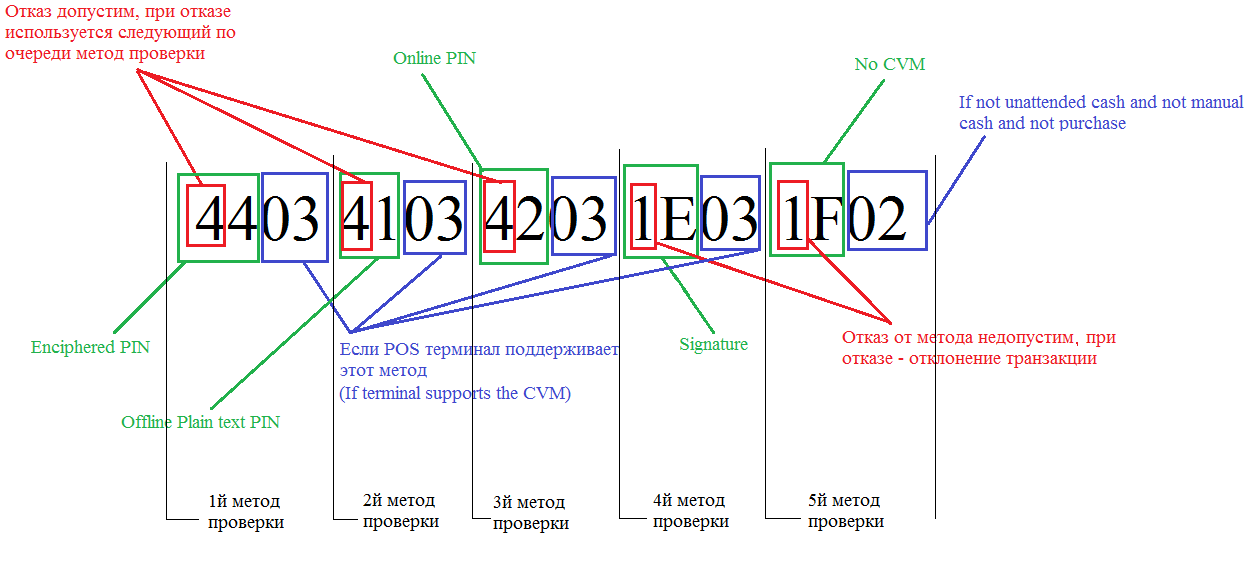
\includegraphics[width=0.9\textwidth]{images/research/cvm_check}
    \caption{\centering Расшифрока CVM списка}
    \label{fig:cvm_check}
\end{figure}

Данному примеру соответствует следующий алгоритм действий (при условии совпадения наличия методов):

\begin{enumerate}
    \item запрос PIN карты,
    \item если пользователь отказывается (а он имеет право отказаться)~--- запрос открытого офлайн-PIN,
    \item если снова отказывается~--- запрос онлайн-PIN, который проверяется не картой, а хостом,
    \item если снова отказался~--- запрос подписи (от ее ввода уже невозможно отказаться).
\end{enumerate}

Если в CVM-листе терминала не указан метод <<проверка по подписи>>~--- тогда он пропускается, и это не приравнивается к отказу выполнения транзакции, потому что в таком случае используется метод <<No CVM>> с условием «If not unattended cash and not manual cash and not purchase».
Если и этого метода в CVM-листе терминала нет~--– то проверка неудачная и транзакция отклоняется~\cite{habr_cvm}.


\subsubsection{Стандарт ISO/IEC 14443}

ISO/IEC 14443 - это международный стандарт, описывающий требования к технологиям бесконтактной идентификации, используемой в смарт-картах и
RFID-устройствах. 
Этот стандарт охватывает физические характеристики карт, протоколы передачи данных и методы антиколлизии~\cite{iso_14443}.
Основное применение данный стандарт нашел в сфере бесконтактных платежей посредством банковских карт.
Помимо этого он используется в электронных проездных, а также удостоверениях личности и электронных паспортах.

Обмен информации основан на принципе индуктивной связи между антенной модуля и антенной карты.
Под антенной понимается замкнутая металлическая катушка, способная принимать и излучать электромагнитные волны.
Дальность взаимодействия бесконтактной связи составляет до 10 см, а скорость передачи данных варьируются в диапазон от 106 до 848 кбит/с.

ISO 14443 разделяется на четыре части:

\begin{enumerate}
    \item физические характеристики: содержит описание размеров, материалов и формы карт (обычно формата ID-1, аналогичного банковским картам);
    \item радиоинтерфейс: определяет электромагнитные параметры, включая метод модуляции и демодуляции сигнала;
    \item инициализация и методы антиколлизии: описывает, как карты идентифицируются, и как модуль выбирает конкретную карту из множества доступных (например, в очереди пользователей);
    \item протокол обмена данными: устанавливает правила взаимодействия между картой и модулем, включая форматы команд и структуру данных, содержит описание Half-duplex block transmission protocol~--- протокола, разработанного в соответствии с принципом многоуровневости модели OSI, предназначенного для минимизации взаимодействия карты и модуля, описывая правила между границами уровней данной модели и количества уровней~\cite{iso_14443_en}.
\end{enumerate}


На данный момент существует 2 версии данного стандарта: A и B.
Изначально был разработан стандарт А, однако он обладал недостатками в виде ограниченной производительности и совместимости.
Версия B была разработана позже с целью их исправления.
Устройство на базе версии B данного стандарта обладает большей технической сложностью, а его стоимость выше, чем у устройств ана базе версии A.
Поэтому наиболее широкое применение по-прежнему остается за стандартом A.
Именно он используется в сфере банковских платежей с помощью бесконтактных карт.
Тип B чаще используется в более сложных системах, где необходимо передавать больший объем данных, и имеется больше требований безопасности.
Примерами таких систем выступают:

\begin{itemize}
    \item электронные паспорта (ePassports),
    \item удостоверения личности,
    \item медицинские карты.
\end{itemize}

Основные отличия технологий A и B приведены в таблице~\ref{tab:iso14443_comparison}.

\begin{table}[H]
    \caption{Сравнительная характеристика стандартов ISO 14443-A и ISO 14443-B}
    \label{tab:iso14443_comparison}
    \begin{sloppypar}
        \centering
        \begin{tabularx}{\textwidth}{ | >{\raggedright\arraybackslash}X | >{\raggedright\arraybackslash}X | >{\raggedright\arraybackslash}X | }
            \hline
            \textbf{Характеристика} & \textbf{ISO 14443-A} & \textbf{ISO 14443-B} \\
            \hline
            Метод модуляции & Amplitude Shift Keying (ASK) & Binary Phase Shift Keying (BPSK) \\
            \hline
            Скорость передачи & 106 кбит/с & 106, 212, 424, 848 кбит/с \\
            \hline
            Антиколлизия & Использует метод <<первый пришёл>> & Использует временные слоты и уникальные идентификаторы \\
            \hline
            Стабильность питания & Низкая & Высокая \\
            \hline
            Устойчивость к помехам & Высокая защита от помех & Уязвимость к внешним воздействиям \\
            \hline
        \end{tabularx}
    \end{sloppypar}
\end{table}


\paragraph{ISO/IEC 14443--3}

ISO/IEC 14443--3 описывает третий уровень стандарта ISO/IEC 14443, который фокусируется на установлении связи между устройствами считывания (PCD - Proximity Coupling Device) и бесконтактными картами (PICC - Proximity Integrated Circuit Card).
Данный уровень определяет механизмы обнаружения карт, установления связи и антиколлизии.
Этот уровень является критически важным для правильной работы систем, где одновременно могут находиться несколько карт в зоне действия ридера~\cite{iso14443-3}.

Антиколлизия (anti-collision) в контексте стандарта ISO/IEC 14443-3~--- это механизм, позволяющий устройству чтения (PCD) корректно идентифицировать и взаимодействовать только c одной картой (PICC) в случае, когда несколько бесконтактных карт находятся в зоне действия считывателя.

Стандарт ISO/IEC 14443--3 описывает следующие аспекты взаимодействия PCD и PICC:

\begin{itemize}
    \item процесс обнаружения карт (Polling): обнаружение карт PCD, которые входят в поле его действия;
    \item формат байтов, кадры и временные характеристики: правила формирования кадров данных и временные интервалы передачи, которые должны соблюдаться для корректной передачи информации между устройствами;
    \item антиколлизионные методы: способы обнаружения и выбора одной карты из нескольких, находящихся в зоне действия ридера;
    \item инициализация связи: начальная команда запроса, корректный ответ на запрос и ошибки соединения, а также параметры, необходимые для начала взаимодействия между PCD и PICC.
\end{itemize}

В соответствии со стандартом определена диаграмма состояний бесконтактной карты, представленная на рисунке~\ref{fig:picc_states}, она является конечным автоматом.

\begin{figure}[H]
    \centering
    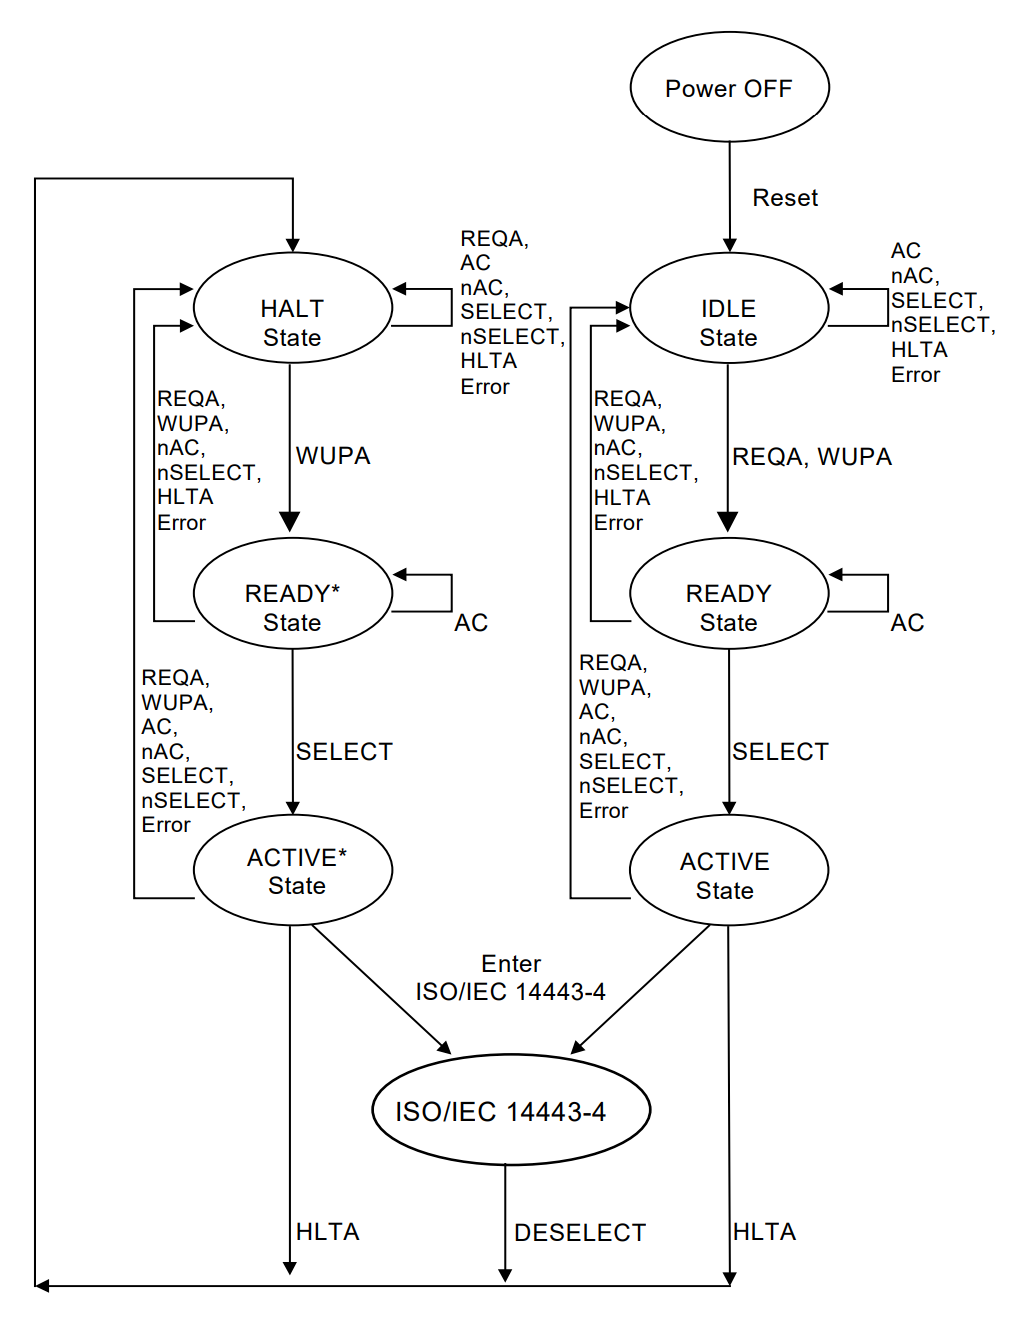
\includegraphics[width=0.5\textwidth]{images/research/picc_states}
    \caption{\centering Диаграмма состояний бесконтактой карты с интегральной схемой}
    \label{fig:picc_states}
\end{figure}

Как видно из рисунка~\ref{fig:picc_states}, бесконтактная карта с интегральной схемой имеет несколько основных состояний:

\begin{itemize}
    \item Power OFF: состояние выключения,
    \item IDLE и HALT: состояния ожидания, которым свойственно низкое потребление электроэнергии,
    \item READY и READY*: состояния готовности к работе,
    \item ACTIVE и ACTIVE*: основные рабочие состояния, в которых доступен функционал, описанный в ISO 14443--4.
\end{itemize}

Также в соответствии со стандартом определен алгоритм работы устройства PCD, который представлен на рисунке~\ref{fig:pcd_flow}.
На нем изображена последовательность работы устройства считывания.

\begin{figure}[H]
    \centering
    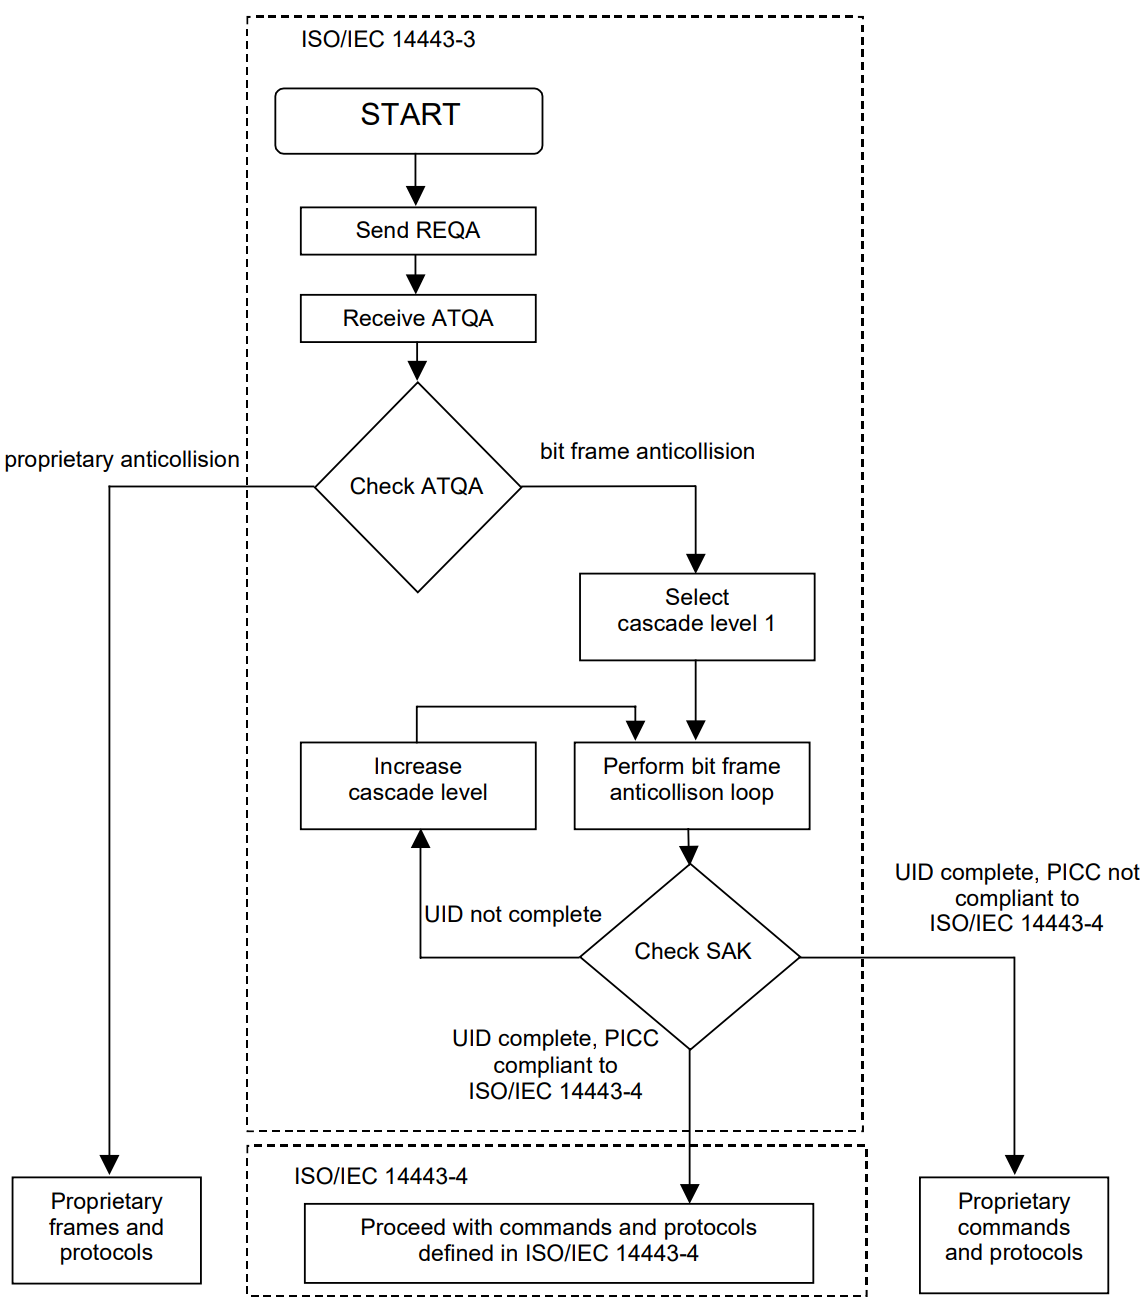
\includegraphics[width=0.7\textwidth]{images/research/pcd_flow}
    \caption{\centering Алгоритм работы устройства-считывателя}
    \label{fig:pcd_flow}
\end{figure}


На рисунках~\ref{fig:picc_states} и~\ref{fig:pcd_flow} приводятся следующие команды и процедуры, с помощью которых происходит взаимодействия PICC и PCD (приписка <<A>> обозначает, что данная команда предназначена для карт, взаимодействующих по стандарту ISO/IEC 14443-A):

\begin{itemize}
    \item REQA (Request A)~--- команда, отправляемая устройством считывания (PCD) для инициирования взаимодействия с картой (PICC), находящейся в состоянии <<IDLE>>, предназначена для проверки наличия карты в пределах досягаемости;
    \item WUPA (Wake-Up A)~--- команда для пробуждения карты из состояния <<HALT>>, используется, если карта находится в режиме ожидания и должна быть возвращена в активное состояние;
    \item AC (Anti-collision)~--- процедура антиколлизии, используемая для выбора одной карты из нескольких, находящихся в зоне действия устройства считывания, позволяет идентифицировать уникальный идентификатор карты (UID);
    \item nAC (Negative Anti-collision)~--- действие обратное процедуре антиколлизии, указывающее, что карта не была выбрана или произошла ошибка во время антиколлизионного процесса;
    \item SELECT~--- команда выбора карты, завершает процесс антиколлизии и устанавливает карту в активное состояние, после выполнения этой команды карта готова к обмену данными;
    \item nSELECT (Negative Select)~--- отрицательная команда выбора, применяемая при ошибке во время процесса выбора карты;
    \item HLTA (Halt A)~--- команда, переводящая карту в состояние <<HALT>>, в этом состоянии карта не отвечает на команды до получения команды WUPA;
    \item Error~--- состояние или ответ, возникающий в случае некорректного выполнения команды или нарушения последовательности команд;
    \item DESELECT~--- команда для завершения активного состояния карты, переводя её обратно в состояние <<IDLE>>;
    \item Enter ISO/IEC 14443--4~--- процесс, переводящий карту в следующий уровень протокола -- ISO/IEC 14443--4.
\end{itemize}


\paragraph{ISO/IEC 14443--4}

ISO/IEC 14443--4 описывает полудуплексный протокол передачи данных блочного типа (half-duplex block transmission protocol).
В данном стандарте определяются последовательности активации и деактивации протокола, а также обеспечивается взаимодействие с другими частями стандарта ISO/IEC 14443.

В данной части стандарта описана поддержка передачи блоков данных прикладного уровня (Application Protocol Data Units, APDUs), описанных в ISO/IEC 7816--4.
Что позволяет осуществлять сопоставление данных в формате APDU и использовать механизмы выбора приложений в соответствии с ISO/IEC 7816--5~\cite{iso_14443_en}.

В данной части протокола подробно описана активация PICC с помощью устройства PCD, схема активации приведена на рисунке~\ref{fig:pcd_flow_2_picc_activation}.


\begin{figure}[H]
    \centering
    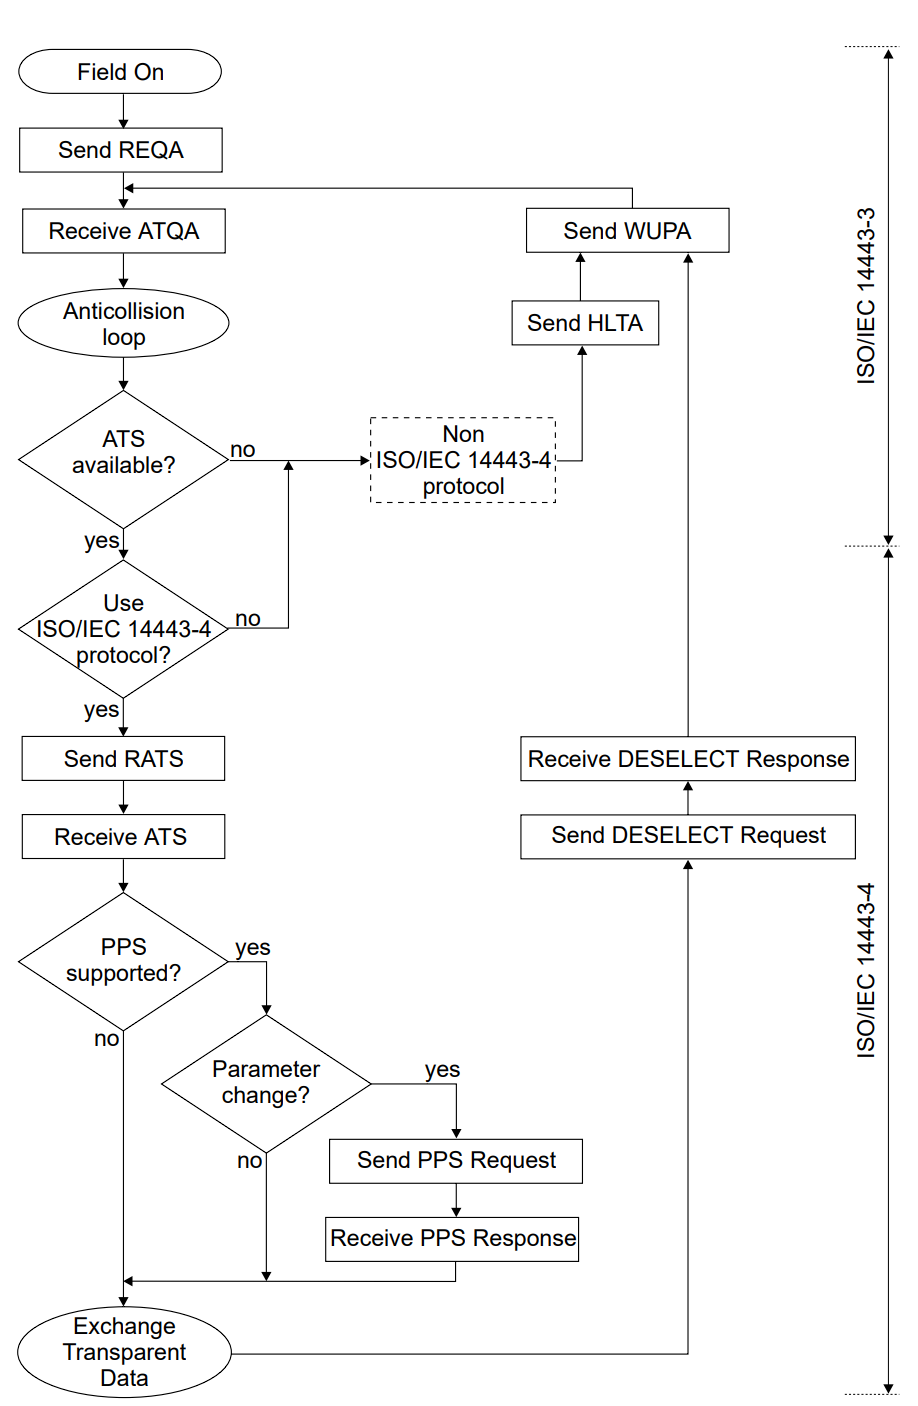
\includegraphics[width=0.7\textwidth]{images/research/pcd_flow_2_picc_activation}
    \caption{\centering Активация бесконтактной карты с помощью PCD}
    \label{fig:pcd_flow_2_picc_activation}
\end{figure}

Данный алгоритм в дополнение к действия, рассмотренным в ISO/IEC 14443--3, описывает действия, которые необходимо сделать для активации полудуплексного протокола передачи данных.
Важно отметить, что отправка RATS (Request for Answer To Select) на PCD в качестве следующей команды происходит после получения SAK, а также, что PICC отвечает на RATS~--- ATS (Answer To Select), это происходит только в том случае, если RATS получен непосредственно после выбора PICC.

Каждый бит RATS, ATS, PPS детально описан в 5 разделе ISO 14443--4~\cite{iso14443-4} Однако дополнительная информация также содержится в спецификации бесконтактного взаимодействия по стандарту EMV, в частности в разделе 10~\cite{emv_specifications_book}.

Half-duplex block transmission protocol~--- полудуплексный протокол передачи данных в виде блоков (кадров).
Он учитывает особые потребности внешнего окружения бесконтактных карт и использует определенный формат кадра, представленный на рисунке~\ref{fig:hd_block_format}.
Кадр состоит из поля пролога (обязательного), информационного поля (необязательного) и поля эпилога (обязательного).

\begin{figure}[H]
    \centering
    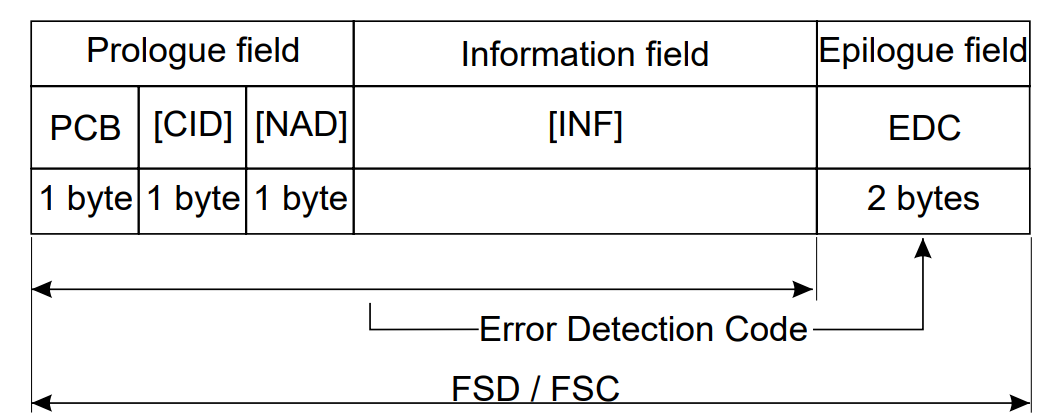
\includegraphics[width=0.5\textwidth]{images/research/hd_block_format}
    \caption{\centering Стандартный формат кадра Half-duplex block transmission protocol}
    \label{fig:hd_block_format}
\end{figure}

Каждый бит элементов данного кадра детально описан в 7 разделе ISO 14443--4~\cite{iso14443-4}.
Дополнительная информация, также содержится в спецификации стандарта EMV, в частности в разделе 10~\cite{emv_specifications_book}.


\subsubsection{ISO 7816}
\label{subsubsec:7816}

ISO/IEC 7816~--- это международный стандарт, который регулирует использование интегрированных схем (ИС) в картах, известных как смарт-карты.
Он охватывает различные аспекты смарт-карт, включая их физические характеристики, электрические интерфейсы, протоколы передачи данных и др..
Стандарт состоит из 15 частей, каждая из которых фокусируется на каком-либо аспекте~\cite{7816_wiki}.

Основное преимущество стандарта ISO/IEC 7816~--- способность обеспечивать совместимость между продуктами различных производителей.
Это достигается благодаря четким спецификациям, которые позволяют разработчикам создавать устройства и приложения, совместимые с картами, соответствующими этому стандарту.

\paragraph{APDU}

APDU (Application Protocol Data Unit)~--- это формат команд и ответов, используемый для взаимодействия между считывателями карт, например, платежными терминалами, и смарт-картами, в том числе банковскими картами с поддержкой технологии EMV.
Команды данного формата определены в стандарте ISO/IEC 7816 и разделены на два типа:

\begin{itemize}
    \item Command APDU~--- команда от терминала к карте;
    \item Response APDU~--- ответ от карты терминалу.
\end{itemize}


APDU-команды используются для передачи инструкций, таких как выбор приложения, запрос информации о карте, выполнение транзакций, чтение данных, а также запись информации на карту.
Важно отметить, что за счет APDU протокол ISO/IEC 7816 позволяет взаимодействовать с контактными картами как и с бесконтактными, посредством использования определенных команд.
Такая гибкость использования стандарта достигается за счет абстрагирования над другими протоколами взаимодействия, упомянутых в предыдущих разделах.

Команда APDU состоит из двух основных компонентов: заголовок и данные.
Более детальная структура представлена на рисунке~\ref{fig:apdu_com}.

\begin{figure}[H]
    \centering
    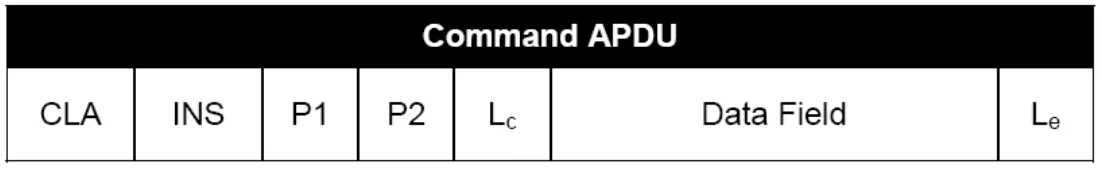
\includegraphics[width=0.7\textwidth]{images/research/apdu_com}
    \caption{\centering Структура APDU команды}
    \label{fig:apdu_com}
\end{figure}


APDU команда (APDU Command) разделяется на следующие элементы~\cite{medium_apdu2}:

\begin{itemize}
    \item CLA (Class): класс инструкции, определяет класс команды и используется для указания типа команды, которую карта должна выполнить;
    \item INS (Instruction): тип инструкции (например, SELECT, READ RECORD), определяет конкретную команду, которую должна выполнить карта;
    \item P1 и P2: параметры для команды (например, указание файла, записи), предоставляют дополнительную информацию или данные для адресации внутри карты;
    \item Lc: длина поля данных команды, если данные присутствуют (необязательный элемент);
    \item  Data (если применимо для команды): данные, специфичные для команды, которые необходимо отправить на карту (например, идентификатор приложения);
    \item Le: ожидаемая длина ответа от карты (необязательный элемент).
\end{itemize}


Структура APDU ответа (APDU Response) представлена на рисунке~\ref{fig:apdu_resp}.

\begin{figure}[H]
    \centering
    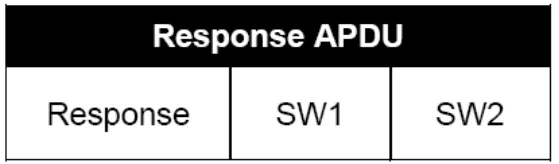
\includegraphics[width=0.5\textwidth]{images/research/apdu_resp}
    \caption{\centering Структура APDU ответа}
    \label{fig:apdu_resp}
\end{figure}

В состав APDU ответа входят следующие элементы:

\begin{itemize}
    \item Data: данные, отправленные картой в ответ на команду;
    \item SW1 и SW2 (Status Words): двухбайтовые коды статуса, указывающий результат выполнения команды.
\end{itemize}

Наиболее распространенными ответами являются <<90:00>>, означающий успешное выполнение, и <<6A:82>>~-- ошибка поиска файла или приложения~\cite{apdu_resp}.


\paragraph{Прикладное применение APDU}

Для инициализации транзакции между картой и терминалом, обмена данными и завершения процесса необходимо следовать определенной последовательности APDU команд.

Cписок стандартных APDU команд ISO 7816--4, в т.ч. используемых в стандарте EMV, приведен на рисунке~\ref{fig:apdu_commands}~\cite{iso7816-4}.

\begin{figure}[H]
    \centering
    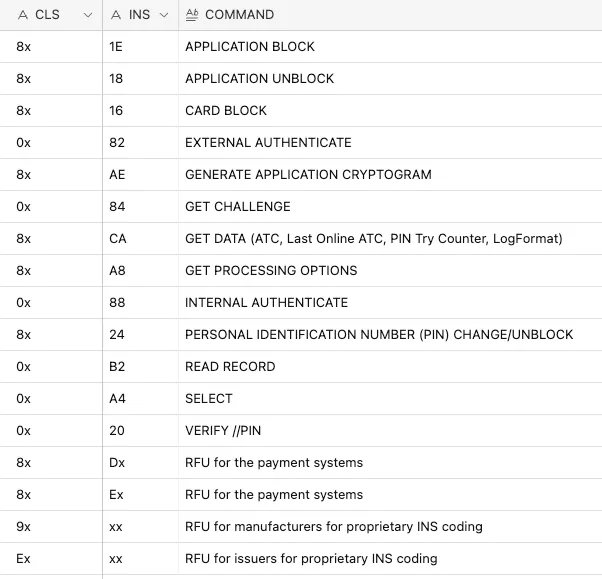
\includegraphics[width=0.7\textwidth]{images/research/apdu_commands}
    \caption{\centering Список APDU команд, используемых при взаимодействии карты и терминала}
    \label{fig:apdu_commands}
\end{figure}

APDU-команды могут быть использованы для выбора приложения на банковской карте и для последующей работы с ним.
Есть приложения, в т.ч. платежные, которые способны взаимодействовать с данными в памяти карты.
С их помощью можно запросить информацию, содержащую различные данные карты, например ее срок действия карты, уникальный номер и пр.
Таким образом во время выполнения платежной транзакции получаются все необходимые данные.
Для подобных целей обычно используется команда READ RECORD, после предварительного выбора приложение для работы с памятью по его AID.
Для выбора конкретного приложения необходимо указать AID (Application Identifier) при использовании команды SELECT.
В ответе на данную команду карта сообщает об успешном или неуспешном выборе приложения~\cite{medium_apdu2_1}.


\subsubsection{Технология NFC}

Near-field communication (NFC) - это технология беспроводной связи малого радиуса действия, которая позволяет передавать данные между двумя устройствами, находящимися на расстоянии до 20 сантиметров.
Данная технология представляет собой набор протоколов связи, которые обеспечивают низкоскоростное соединение с простым и быстрым подключением.
Подобно другим технологиям карт ближнего взаимодействия, NFC основана на индуктивной связи между двумя электромагнитными катушками, встроенными в устройства с поддержкой NFC, такие как смартфоны.
Для обмена данными в одном или обоих направлениях NFC использует частоту 13,56 МГц, находящуюся в глобально доступном нелицензируемом диапазоне ISM (Industrial, Scientific and Medical).
Этот стандарт соответствует спецификации ISO/IEC 18000--3 и поддерживает скорости передачи данных от 106 до 848 кбит/с~\cite{nfc_wiki}.
Данная технология получила широкое применение в сфере бесконтактной оплаты.

Технология NFC охватывает как протоколы связи, так и форматы обмена данными.
Они основаны на существующих стандартах радиочастотной идентификации (RFID), в частности ISO/IEC 14443.
NFC описана в стандарте ISO/IEC 18092 и ряде других стандартов, разработанных объединением <<NFC Forum>>.
Структура данной технологии представлена на рисунке~\ref{fig:nfc_tech}, где изображено разделение на различные слои, начиная с физического уровня и заканчивая уровнем приложений (снизу вверх).
Каждый из описанных уровней связан с определёнными стандартами и обеспечивает целостность работы технологии NFC, начиная с физической передачи сигнала и заканчивая выполнением прикладных задач.

\begin{figure}[H]
    \centering
    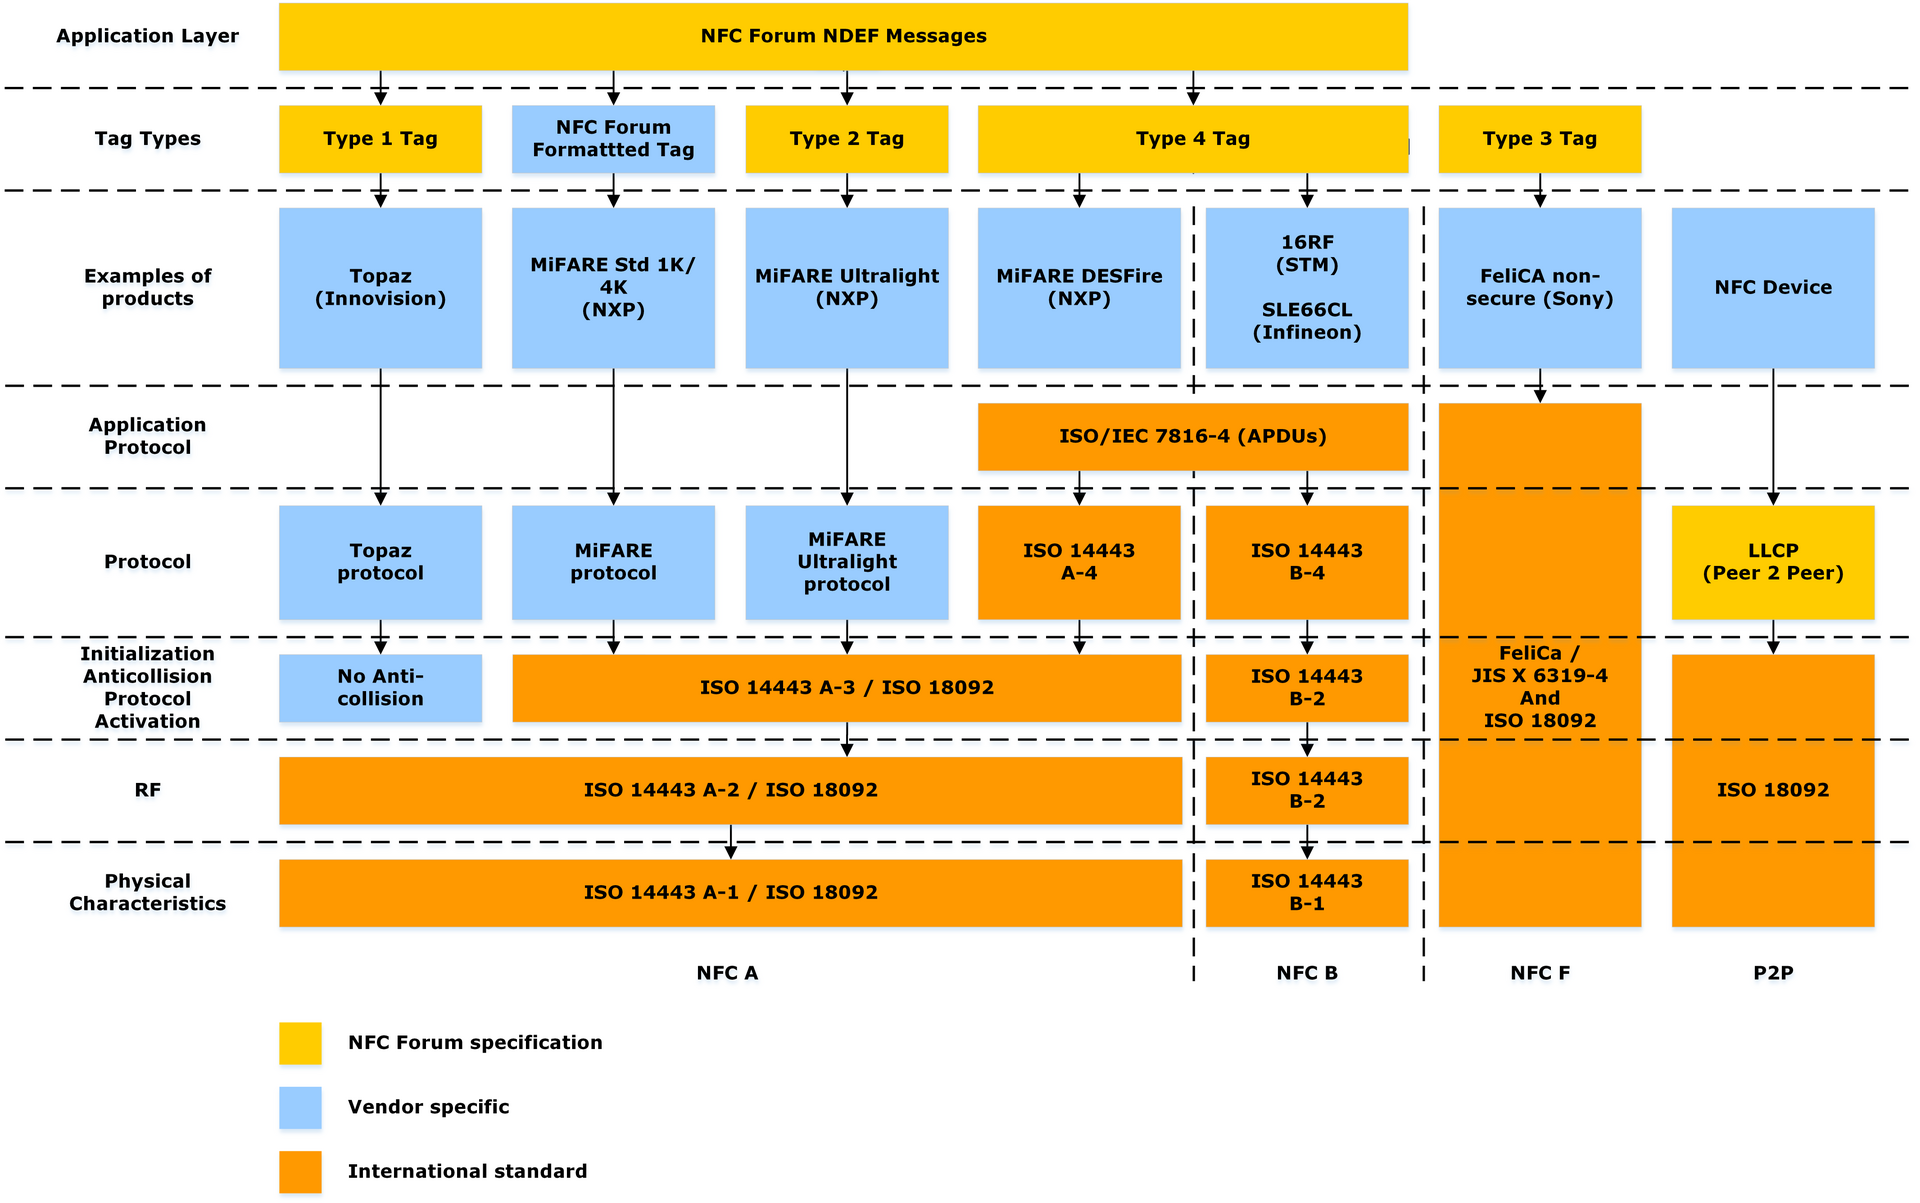
\includegraphics[width=1\textwidth]{images/research/nfc_tech}
    \caption{\centering Стек протоколов NFC}
    \label{fig:nfc_tech}
\end{figure}

Важно, что данная технология реализует ISO/IEC 14443 и ISO/IEC 7816~--- это позволяет устройствам, содержащим модуль NFC 4-го типа (NFC Type 4 Tag) использоваться для бесконтактной оплаты, т.к. данные модули совместимы с терминалами оплаты.





\subsubsection{EMV Contactless}






\subsubsection{3DES}


\subsubsection{MirAccept}


\subsubsection{PCI DSS и PCI PTS}






\subsection{Формирование требований к системе}

На основании классификации платежных устройств от ФСБ РФ и ЦБ РФ, разрабатываемое устройство является <<защищенным считывателем карт для пользовательских устройств (SCRP-устройством)>>, т.к. используется вместе с мобильным пользовательским устройством (смартфоном м или планшетом).



	%\newpage

% Из текста короткого задания на ВКР:
% 1. Определение средств разработки и архитектуры системы: разработка ее структуры;
% 2. определение набора необходимого оборудования, программного обеспечения.

% 3. Проектирование и определение спецификаций аппаратной и программной компонентов системы.
% 4. Реализация компонентов системы с использованием выбранных средств разработки.
% 5. Сборка макета аппаратной подсистемы.
% 6. Сборка, установка и тестирование программного обеспечения аппаратной и программных подсистем.
% 7. Тестирования системы, интеграции программной и аппаратных частей.

\section{Разработка программно-аппаратной системы}

В данном разделе описывается проектирование аппаратной части системы~--- считывателя бесконтактных платежных карт~--- и разработка программной части СБО~--- программного обеспечения для считывателя и мобильного приложение бесконтактной оплаты.
Для этого в соответствии с техническим заданием (ТЗ) решаются следующие задачи:

\begin{itemize}
    \item определение средств разработки и архитектуры системы: разработка ее структуры; определение набора необходимого оборудования, программного обеспечения;
    \item проектирование компонентов и определение спецификаций аппаратной части СБО, сборка макета аппаратной части системы;
    \item выбор архитектуры и подхода разработки программной подсистемы, проектирование программных компонентов СБО (программы мобильного терминала бесконтактной оплаты и мобильного приложения оплаты) и определение спецификаций компонентов;
    \item реализация компонентов системы с использованием выбранных средств разработки;
    \item сборка, установка и тестирование программного обеспечения аппаратной подсистемы и программного обеспечения программной подсистемы.
\end{itemize}

Разрабатываемая система является mPOS-терминалом с поддержкой бесконтактной оплаты.
Как любой mPOS-терминал она состоит из мобильного устройства и считывателя платежных карт, подключаемого к ней.
В соответствии с требованиями ТЗ считыватель поддерживает только бесконтактные карты и подключается беспроводным образов посредством технологии Bluetooth.
Считыватель взаимодействует с платежным средством посредством технологии NFC.

Процесс оплаты с использованием устройства представляет следующую последовательность действия:
\begin{enumerate}
    \item представить торгово-сервисного предприятия (ТСП) вводит данные о платеже в мобильное приложение и активирует считыватель;
    \item держатель карты прикладывает к считывателю средства платежа (карта или мобильное приложение, эмулирующее платежную карту);
    \item считыватель взаимодействует со средством платежа и передает данные, необходимые для формирования платежа, на мобильное устройство;
    \item мобильное устройство отправляет HTTP-запрос на сервер банка-эквайера для выполнения платежа;
    \item сервер банка-эквайера отправляет HTTP-ответ на мобильное устройство, сообщая о статусе операции.
\end{enumerate}

Плательщик (держатель карты) может убрать средство платежа от считывателя после того как считыватель выполнит все необходимые операции для получения данных, необходимых для формирования платежа, либо сообщит о невозможности продолжения транзакции из-за ошибок совместимости или выполнения взаимодействия.


\subsection{Разработка структуры системы}

Структура разрабатываемой системы представлена на рисунке~\ref{fig:struct_scheme}.
Направления стрелок показывают направления обмена данными между программными и аппаратными модулями.

\begin{figure}[H]
    \centering
    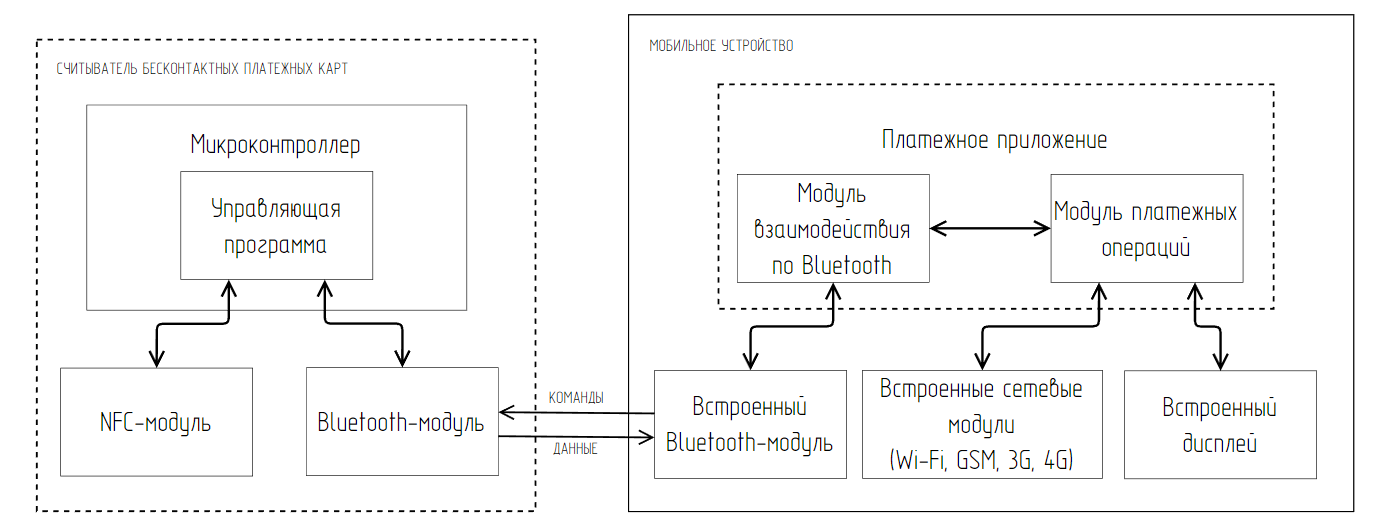
\includegraphics[width=0.8\textwidth]{images/design/struct_scheme}
    \caption{\centering Структурная схема системы}
    \label{fig:struct_scheme}
\end{figure}

Считыватель бесконтактных платежных карт включает в себя 3 аппаратных модуля в соответствии с требованиями ТЗ:
\begin{itemize}
    \item Bluetooth-модуль для связи с мобильным устройством, которое осуществляет выполнения платежных операций;
    \item NFC-модуль для взаимодействия с бесконтактной средством платежа;
    \item микроконтроллер для осуществления управления устройством (контроля работы NFC-модуля и Bluetooth-модуля).
\end{itemize}

Для микроконтроллера реализуется ПО, с помощью которого осуществляется управления NFC и Bluetooth модулями, через предоставляемые модулями интерфейсы для управления, описанных в их документации (форматом управляющих команд).
NFC-модуль подключается посредством разъема SPI, Bluetooth-модуль подключается посредством разъема USART для передачи управляющих команд с необходимыми данными.


Мобильное приложение включает в себя следующие программные модули:
\begin{itemize}
    \item модуль взаимодействия с устройством считывателем по Bluetooth,
    \item модуль платежных операций для сетевых запросов к API банка-эквайера.
\end{itemize}

Используются следующие аппаратные модули мобильного устройства:
\begin{itemize}
    \item Bluetooth-модуль для взаимодействия со считывателем,
    \item встроенные сетевые модули (Wi-Fi, GSM, 3G, 4G) для взаимодействия с сервером банка-эквайера,
    \item дисплей для взаимодействия с пользователем.
\end{itemize}

Структурная схема с внешними участниками процесса оплаты представлена на рисунке~\ref{fig:struct_scheme_out}.
На ней также указаны направления обмена данными между программными, аппаратными модулями и внешними участниками процесса оплаты.

\begin{figure}[H]
    \centering
    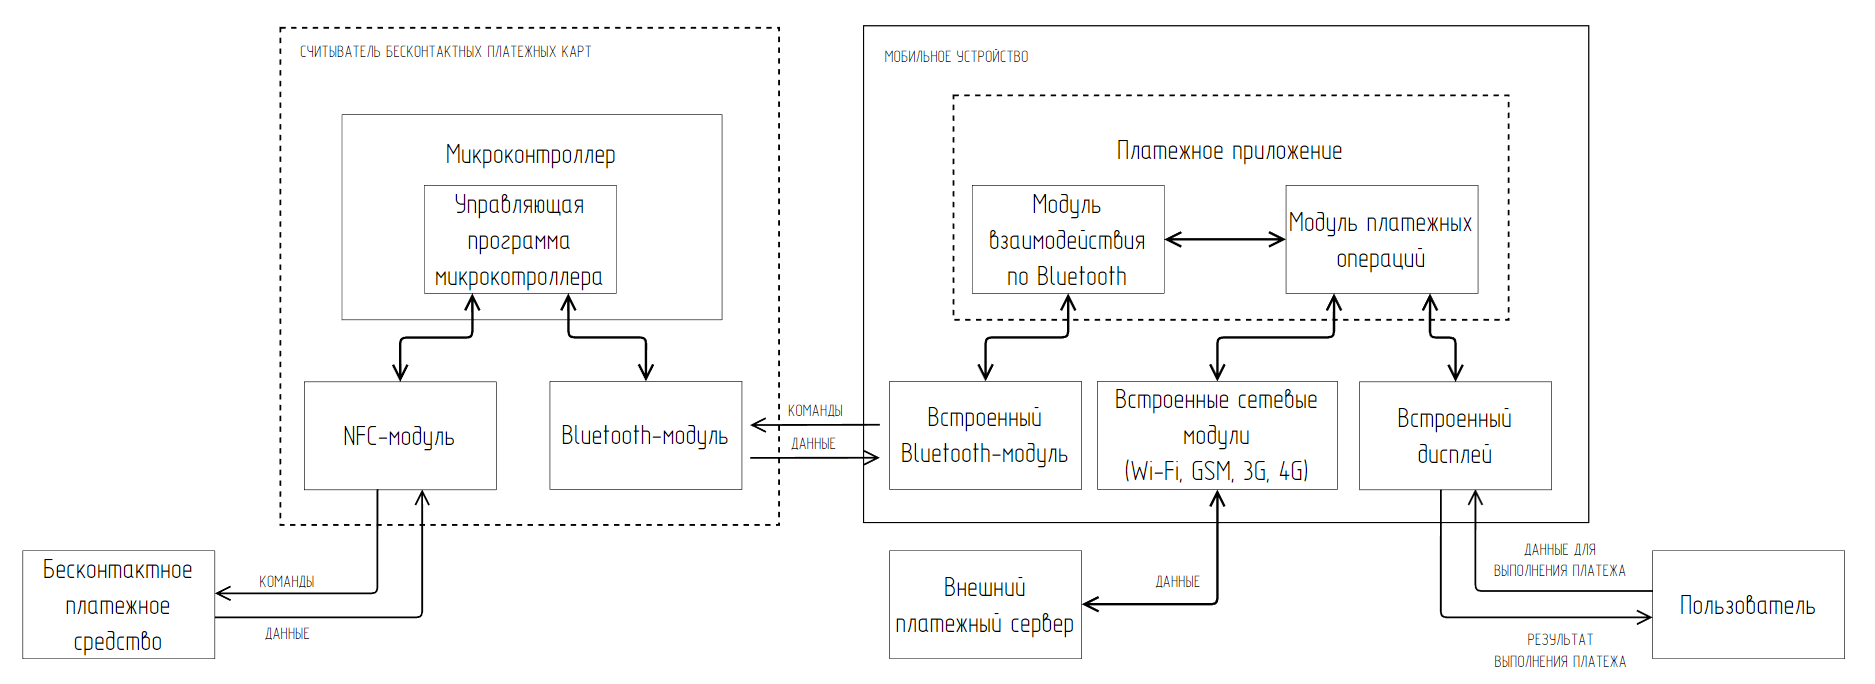
\includegraphics[width=1\textwidth]{images/design/struct_scheme_out}
    \caption{\centering Структурная схема системы с внешними участниками процесса оплаты}
    \label{fig:struct_scheme_out}
\end{figure}


\subsection{Разработка аппаратной части системы}

\subsubsection{Функциональная схема аппаратной части системы}

В соответствии с требованиями технического задания основные функции аппаратной части системы (микроконтроллерной системы):
\begin{itemize}
    \item взаимодействие со средством платежа посредством технологии NFC в соответствии со стандартом взаимодействия с бесконтактными средствами платежа EMV Contactless, рассмотренном в исследовательской части;
    \item связь с мобильным устройством посредством технологии Bluetooth (получение управляющих команд и отправка полученных данных).
\end{itemize}

В данном процессе задействуется МК, Bluetooth-модуль и NFC-модуль.
Все эти компоненты работают как единая система под управлением МК.

Структурная схема устройства представлена на рисунке~\ref{fig:apparat_struct}.
На ней NFC-модуль имеет детализированное изображение с целью демонстрации комплексности структуры данного устройства.

\begin{figure}[h]
    \centering
    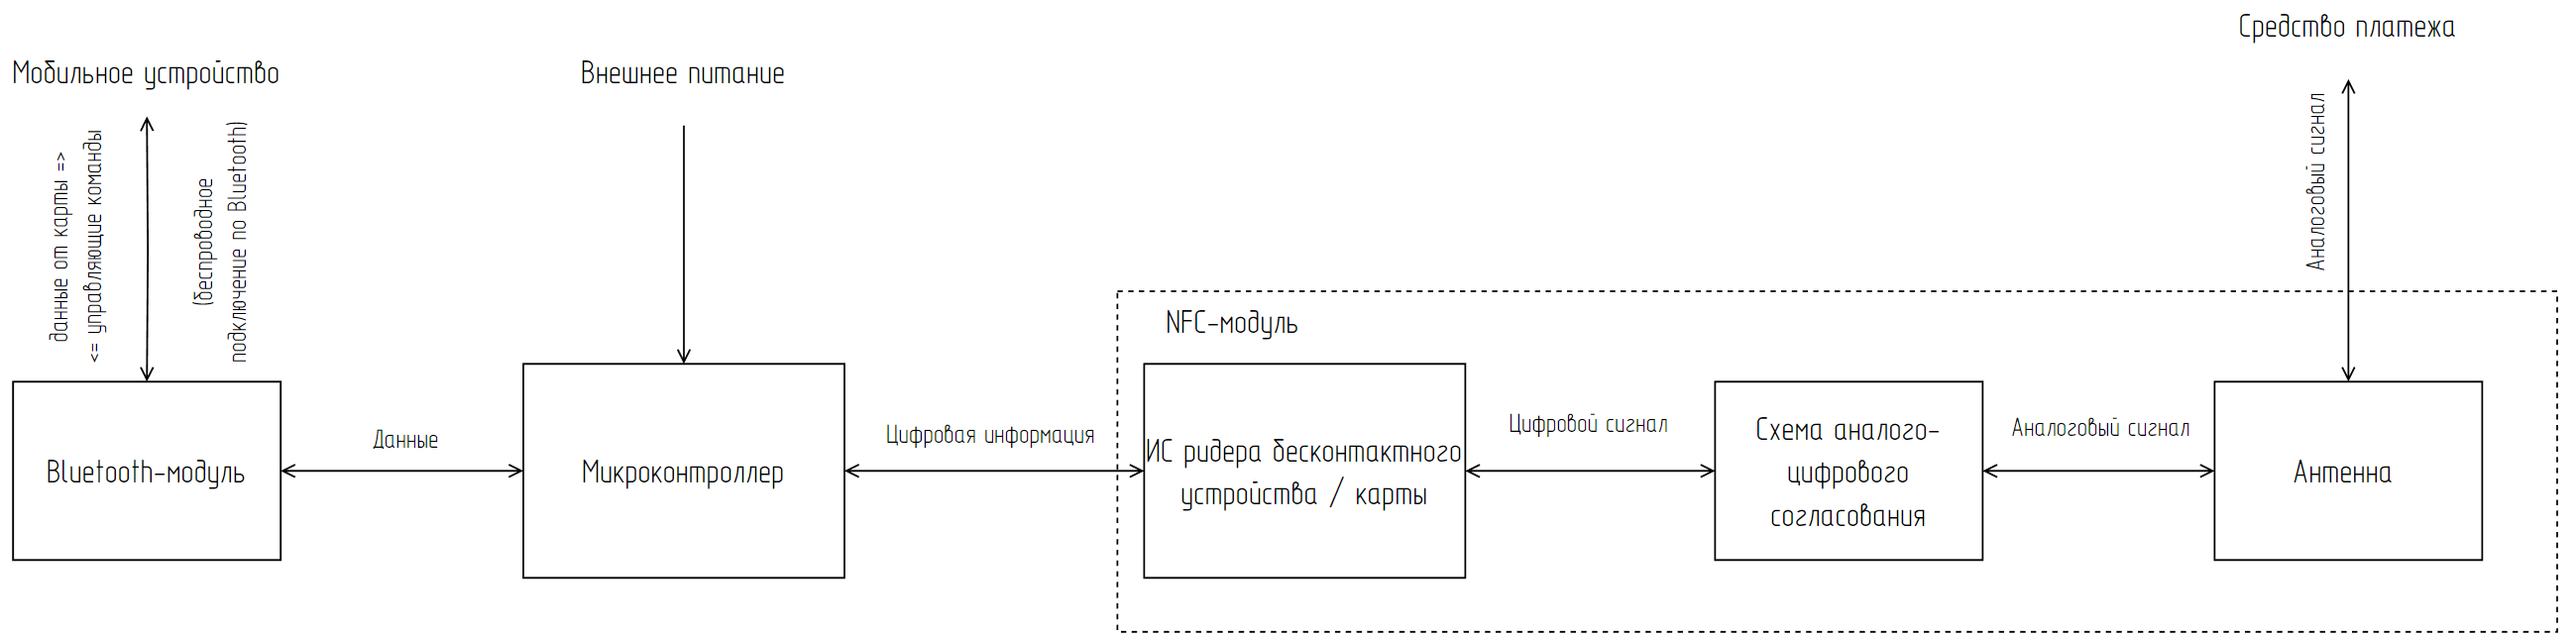
\includegraphics[width=1\textwidth]{images/design/apparat_struct}
    \caption{\centering Структурная схема считывателя бесконтактных платежных карт}
    \label{fig:apparat_struct}
\end{figure}

Согласно требованию ТЗ разрабатываемое устройство должно обеспечивать возможность подключения по Bluetooth к мобильному устройству, с возможностью приема и передачи данных, также оно должно взаимодействовать с бесконтактным средством платежа в соответствии со стандартом ISO/IEC 14443 с помощью модуля NFC, поддерживающему работу с картами ПС <<МИР>>.
Данные модули должны работать под управлением МК, имеющего разъемы SPI и USART для их подключения.
При этом стандарта EMV Contactless вводит строгие временные ограничения на время прямого непосредственного взаимодействия с картой (не более 0.4 мс).
Из чего следует, что МК должен обладать высокой производительностью.
ISO/IEC 14443-A используемый в платежных картах обладает скоростью передачи данных 106 кбит/с или 13.25 кбайт/с, что с учетом используемого компактного формата TLV для передаваемых сообщений и их размера, который значительно меньше чем объем, предаваемый даже за 1 мс, не создает ограничений по производительности.

При анализе существующих mPOS-терминалов было установлено, что они используют микропроцессоры с архитектурой Advanced RISC Machines (ARM), в частности ARM 7, ARM 9, ARM 11, которые обладают частотой более 100 МГц.
С учетом того, что данные терминалы используются для обработки транзакций различных платежных систем и не только бесконтактным образом для разрабатываемой системы данные процессоры будут избыточны, однако использование ARM архитектуры было бы крайне желательно.

В таблице~\ref{tab:microcontroller_comparison} приведены характеристики различных микроконтроллеров от разных компаний~\cite{stm32f103_datasheet}\cite{atmega328p_datasheet}.

\begin{longtable}[l]{|
P{0.18\textwidth}|
P{0.2\textwidth}|
P{0.15\textwidth}|
P{0.13\textwidth}|
P{0.2\textwidth}|}

    \caption{Сравнение характеристик часто используемых микроконтроллеров}
    \label{tab:microcontroller_comparison} \\
    \hline
    \textbf{Характеристика} &
    \textbf{ATmega328P} &
    \textbf{ESP8266} &
    \textbf{PIC16F8} &
    \textbf{STM32F103} \\
    \hline
    \endfirsthead

    \caption*{Продолжение таблицы~\ref{tab:microcontroller_comparison}} \\
    \hline
    \textbf{Характеристика} &
    \textbf{ATmega328P} &
    \textbf{ESP8266} &
    \textbf{PIC16F8} &
    \textbf{STM32F103} \\
    \hline
    \endhead

    \hline
    \endfoot

    \hline
    \endlastfoot

    Разрядность процессора &
    8 бит &
    32 бит &
    8 бит &
    32 бит \\
    \hline

    Тактовая частота &
    до 20 МГц &
    до 160 МГц &
    до 20 МГц &
    до 72 МГц \\
    \hline

    Флэш-память &
    32 КБ &
    4 МБ &
    14 КБ &
    64 КБ \\
    \hline

    SRAM &
    2 КБ &
    160 КБ &
    368 Б &
    20 КБ \\
    \hline

    EEPROM &
    1 КБ &
    Нет &
    256 Б &
    Нет \\
    \hline

    Количество I/O портов &
    23 &
    11 &
    13 &
    37 \\
    \hline

    Поддержка Wi-Fi &
    Нет &
    Да &
    Нет &
    Нет \\
    \hline

    Поддержка Bluetooth &
    Нет &
    Нет &
    Нет &
    Нет \\
    \hline

    Стоимость &
    Низкая &
    Низкая &
    Низкая &
    Низкая \\
    \hline
\end{longtable}

В ходе выполнения курсовой работы по дисциплине <<Микропроцессорные системы>> выбор был сделан в пользу микроконтроллера ATmega328P в составе платы Arduino Uno R3.
Данный вариант был удобен при первоначальном макетировании системы и изучении стандартов взаимодействия бесконтактной карты.
Однако частота данного МК значительно ниже чем у аналогов, у него 8-битная гарвардская архитектура процессора, при прочих равных Flash-памяти, SRAM, количество I/O-портов меньше чем у STM32F103.
Поэтому в качестве МК для аппаратной части системы используется STM32F103C8T6 на базе микропроцессора ARM Cortex-M3 с 32-битной архитектурой.
Данная архитектура позволяет работать с 32-битными регистрами, выполнять сложные математические операции, включая работу с плавающей запятой (с помощью программных или аппаратных средств).
Поддержка современных продвинутых программных библиотек, таких как HAL (Hardware Abstraction Layer), LL (Low Layer) и CMSIS (Cortex Microcontroller Software Interface Standard), предоставляет разработчику полный контроль над аппаратной частью микроконтроллера, с пониманием происходящих процессов на уровне регистров и таймеров.
В то же время, использование ATmega328P с Arduino.h для аналогичных задач часто приводит к неэффективному использованию ресурсов, ограничению функциональности и снижению производительности.
Кроме того, экосистема STM32 предоставляет мощные инструменты разработки, такие как STM32CubeIDE, которые упрощают настройку периферии и генерацию кода, сохраняя при этом гибкость и контроль над аппаратными ресурсами.

Для реализации беспроводного Bluetooth-соединения был выбран Bluetooth-модуль HC-05, обладающий следующими характеристиками:

\begin{itemize}
    \item напряжение питания: 3,3 В – 5 В;
    \item потребляемый ток: при подключении – до 40 мА (поиск, сопряжение, подключение), при передаче данных – до 8 мА;
    \item частотный диапазон: 2,4 ГГц – 2,48 ГГц;
    \item мощность передатчика: до +4 дБм;
    \item дальность связи: до 10 метров;
    \item интерфейс: USART;
    \item поддерживаемые скорости передачи данных: 9600, 19200, 38400, 57600, 115200, 230400 и 460800 бит/сек;
    \item режимы работы: Master (ведущий) и Slave (ведомый);
\end{itemize}

К преимуществам модуля HC-05 относятся дальность связи до 10 метров, поддержка скорости передачи данных до 460800 бит/сек и работа как в режиме Master (ведущий), так и в режиме Slave (ведомый).
Единственным недостатком является не самая актуальная версия технологии Bluetooth 2.0.
Однако даже модуль HC-08 имеет версию 4.0 (актуальная~-- 6.0) при стоимости в 4--5 раз выше и большим энергопотреблением.
Т.к. осуществляется процедура передачи данных без необходимости частого и многоразового подключения устройства-хоста к Bluetooth-модулю, а приоритетом является низкое энергопотребление – стандарт Bluetooth 2.0 является преимуществом, а не недостатком.

Модуль HC-05 можно настроить с помощью AT-команд, которые отправляются через интерфейс USART.
Это позволяет изменить имя устройства, пароль для подключения, скорость передачи данных и другие параметры.
Примеры AT-команд:

\begin{itemize}
    \item AT – проверка связи с модулем;
    \item AT+NAME=NewName – изменение имени модуля;
    \item AT+UART=9600 – установка скорости передачи данных на 9600 бод.
\end{itemize}

Модуль HC-05 включает в себя чип BC417143 и работает на напряжении 5 В и реализуя прием и передачу сигнала.


Среди прочих NFC-модулей наиболее популярными являются модули компании NXP.
К тому они имеют качественную и исчерпывающую документацию.
NXP поставляет не только NFC-модули, но и микроконтроллеры с интегрированными модулями NFC, а также разрабатывает ПО для работы с модулями, однако только для МК собственного производства.

В качестве модуля для считывателя используется NXP PN5180.
Данный модуль имеет поддержку большого числа стандартов технологии NFC.
Имеет сравнительно низкую стоимость (порядка 700--1000 рублей на ноябрь 2024 года).
А также имеет широкий функционал и подробную документацию.
PN5180 является широко распространенным модулем, с поддержкой множества стандартов (в том числе и используемого в платежах~-- ISO14443-A).
Альтернативой ему могут выступать схожие модули от компании NXP, в частности PN5190 (улучшенная версия PN5180), однако он умеет выше стоимость и при этом улучшения в производительности и поддержки стандартов пренебрежимо малы в рамках данного устройства.

%Основные внутренние компоненты интегральной схемы модуля представлены на рисунке~\ref{fig:pn5180_components}~\cite{pn5180_datasheet}.
%
%\begin{figure}[H]
%    \centering
%    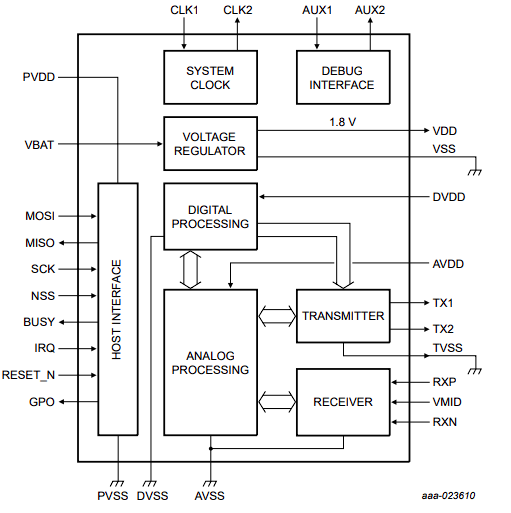
\includegraphics[width=0.8\textwidth]{images/design/pn5180_components}
%    \caption{\centering Компоненты интегральной схемы модуля PN5180}
%    \label{fig:pn5180_components}
%\end{figure}

Важно отметить, что производитель модуля предварительно выполняет следующие действия по его настройке:
\begin{itemize}
    \item определение целевого импеданса для оптимизации мощности RF-выхода и минимизации потребление энергии;
    \item проектирование EMC-фильтра для подавления нежелательных гармоник тока, которые могут создавать помехи в работе устройств;
    \item измерение LCR-параметров антенны (индуктивности, емкости и сопротивления) для работы;
    \item расчет компонентов для согласования антенны с NFC-модулем.
\end{itemize}

Также производится симуляция работы антенны, тестирование работы в реальных условиях и корректировка РЧ контура.
В результате чего получается надежный и стабильно работающий модуль, для которого нет необходимости в выполнении данных затруднительных действий, требующих дополнительного оборудования и навыков.


PN5180 использует для связи с микроконтроллером SPI, расширенный линией BUSY, что позволяет ему указыать о невозможности приема и отправки данных в конкретный момент времени.
Максимальная скорость его разъема SPI составляет 7 Мбит/с, при этом параметры SPI устанавливаются следующим образом: CPOL=0, CPHA=0 (SPI Mode 0), старший бит первым (MSB first).
На модуль по SPI передаются управляющие команды, список которых приведен в его datasheet в разделе <<Работа модуля NFC>>, с помощью этих команд происходит настройка модуля\cite{pn5180_datasheet}.

Уровень напряжения сигналов, которыми оперирует модуль, составляет 1,8--3,3 В.
У STM32F103C8T6 рабочий уровень напряжения на разъемах~--- 3,3 В, что делает его совместимым с данным модулем.
В свою очередь на разъемах микроконтроллера ATmega328P рабочим уровнем напряжения является 5 В, что усложняло его использование в первом разработанном макете устройства (возникала необходимость использования конвертера уровня напряжения, что повышало количество энергии, потребляемое МК-системой).


На функциональной схеме изображены используемые компоненты, необходимые для работы устройства, также показаны подключения модулей и используемые для этого контакты, направления передачи данных и управляющих сигналов.
Спроектированная функциональная схема разработанного устройства представлена в приложении~В.
На схеме МК изображены только используемые компоненты.




\subsubsection{Принципиальная схема аппаратной части системы}

%\paragraph{Программирование МК}

Программирование микроконтроллера STM32F103C8T6 осуществляется с использованием интерфейса SWD (Serial Wire Debug), который является стандартным решением для отладки и прошивки большинства 32-битных ARM-микроконтроллеров.
Интерфейс SWD разработан для упрощенного подключения к микроконтроллеру, в отличие от JTAG, он использует минимальное количество выводов, что делает его особенно удобным в условиях ограниченного пространства на плате.

Для работы с этим интерфейсом необходимы всего два сигнальных контакта:
\begin{itemize}
    \item SWCLK — тактовая линия;
    \item SWDIO — двунаправленная линия передачи данных.
\end{itemize}

Также требуются линии питания и земли:
\begin{itemize}
    \item VCC — питание 3.3 В;
    \item GND — общий провод.
\end{itemize}

Процесс программирования выглядит следующим образом:

\begin{enumerate}
    \item программатор ST-Link v2 подключается к микроконтроллеру через разъем, соответствующий интерфейсу SWD;
    \item программатор устанавливает связь с ядром микроконтроллера, отправляя тактовые сигналы по линии SWCLK и управляя данными через SWDIO;
    \item происходит загрузка и запись кода во флэш-память микроконтроллера;
    \item МК автоматически перезапускается для исполнения загруженную программы.
\end{enumerate}

Таким образом, для программирования микроконтроллера через ST-Link v2 используется разъем SWD, представленный на рисунке~\ref{fig:swd}.

\begin{figure}[H]
    \centering
    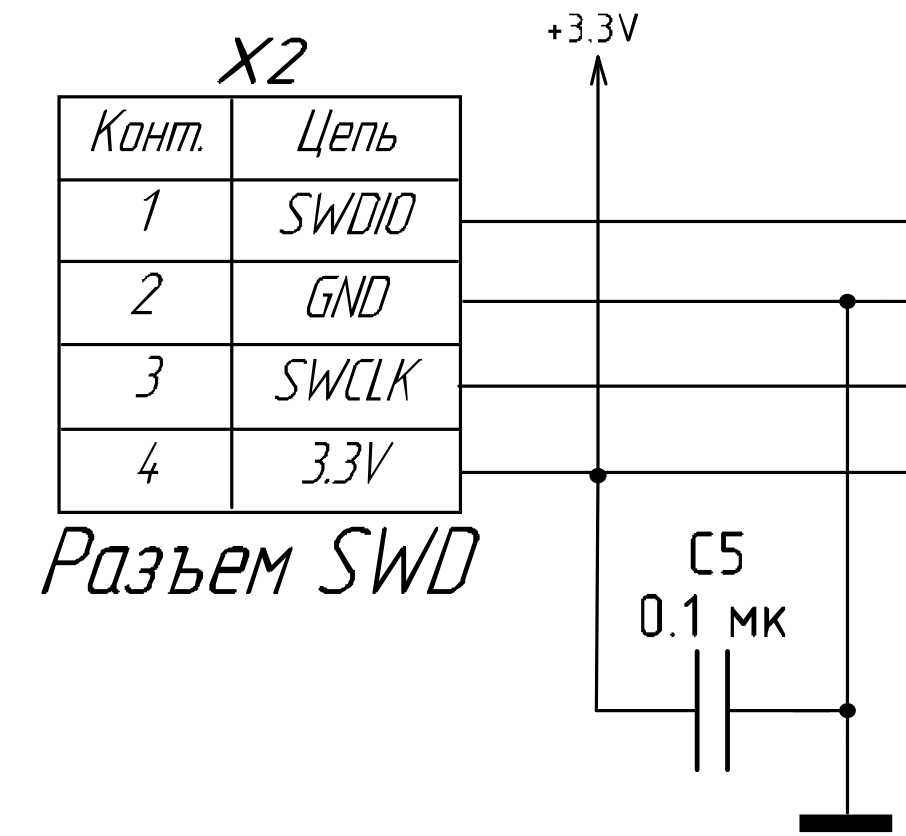
\includegraphics[width=0.3\textwidth]{images/design/swd}
    \caption{\centering Разъем программирования МК}
    \label{fig:swd}
\end{figure}

%\paragraph{Подключение цепи питания}

Для обеспечения работоспособности устройства необходимо подавать стабилизированное напряжение на микроконтроллер и прочие компоненты схемы.
В данной МК-систем питание микроконтроллера STM32F103C8T6 осуществляется через стандартный USB-разъём microUSB, который используется как интерфейс подключения к внешнему источнику питания.
Это позволяет отказаться от использования дополнительного внешнего источника питания и упрощает конструкцию устройства.
Разъем представлен на рисунке~\ref{fig:usb}.

\begin{figure}[H]
    \centering
    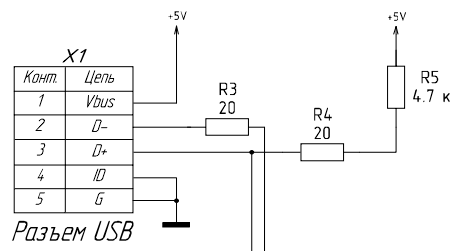
\includegraphics[width=0.4\textwidth]{images/design/usb}
    \caption{\centering Разъем питания МК}
    \label{fig:usb}
\end{figure}

Напряжение с USB поступает непосредственно на стабилизатор напряжения RT9193--33, т.к. микроконтроллер STM32F103C8T6 работает на напряжении 3.3 В, а не 5 В, как это часто бывает в других МК.
Стабилизатор преобразует напряжение с USB (5 В) к необходимому уровню и обеспечивает стабильное питание ядра и периферийных модулей микросхемы.

Для фильтрации питающего напряжения используются керамических конденсаторы, установленные на входе и выходе стабилизатора.
Такое решение обеспечивает минимальный уровень шума и стабильную работу микроконтроллера.
Емкости конденсаторов определены в соответствии с документацией STM32F103C8T6~\cite{stm32f103_datasheet}.

Схема стабилизации и понижения напряжения представлена на рисунке~\ref{fig:mk_usb_stab}.

\begin{figure}[H]
    \centering
    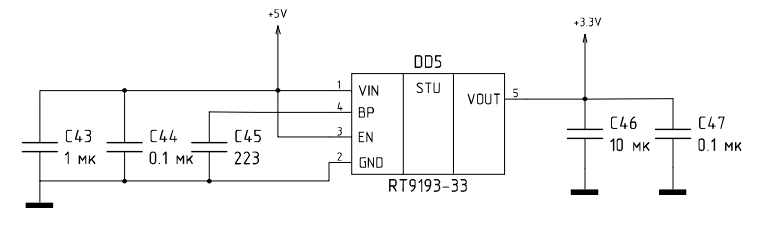
\includegraphics[width=0.6\textwidth]{images/design/mk_usb_stab}
    \caption{\centering Схема стабилизации питания МК-системы}
    \label{fig:mk_usb_stab}
\end{figure}

%\paragraph{Расчет сопротивления резисторов}

На принципиальной схеме расположено несколько резисторов.

Резистор R1 используется для стабилизации тока на источнике тактирования.
Резистор R2 используется для подтягивания линии RESET до 3.3~В.
Их номиналы установлены согласно документации на микроконтроллер\cite{stm32f103_datasheet}.

Резисторы R2--R5 добавлены для токоорганичния разъема USB, который используется для питания.

В Bluetooth-модуле, согласно документации, резисторы R6, R9 имеют номинал 220~кОм и 1~кОм соответственно, а R7, R8~--- 10~кОм.

В состав NFC-модуля PN5180, согласно документации, входят резисторы R10, R11 сопротивлением 4.7 кОм и R12--R15 сопротивлением 2.2~кОм.

Дополнительно хотелось бы отметить, что расчет сопротивлений, емкостей и индуктивностей для PN5180 производился на основе раздела datasheet <<17.1 Typical component values>>\cite{pn5180_datasheet}.
В нем приведена схема с минимальным количеством компонентов и значения для них.
Схема представлена на рисунке~\ref{fig:pn5180mincomp}, значения для нее на рисунке~\ref{fig:pn5180mincompvalues}.

\begin{figure}[H]
    \centering
    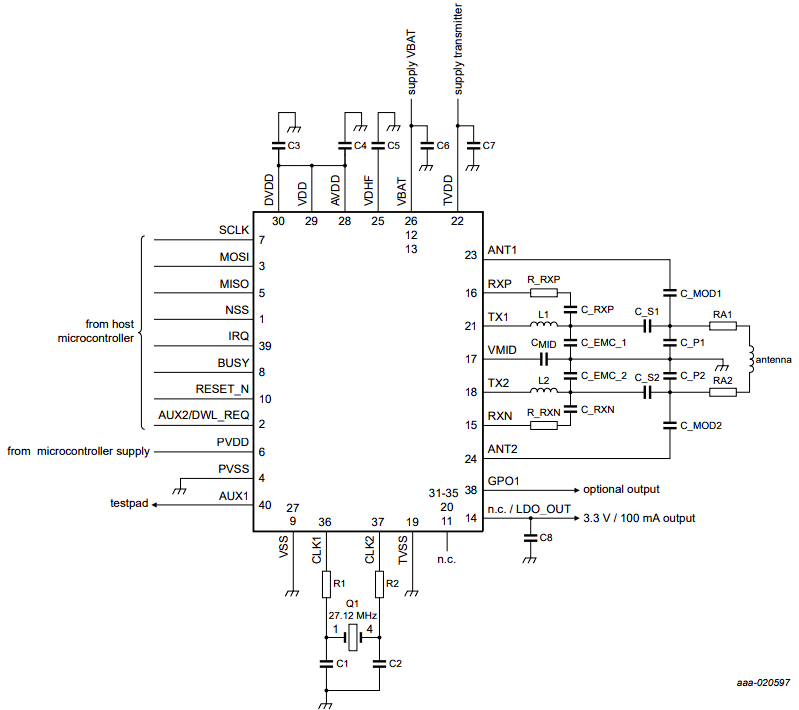
\includegraphics[width=0.7\textwidth]{images/design/pn5180mincomp}
    \caption{\centering Схема модуля PN5180 с минимальным набором элементов}
    \label{fig:pn5180mincomp}
\end{figure}

\begin{figure}[H]
    \centering
    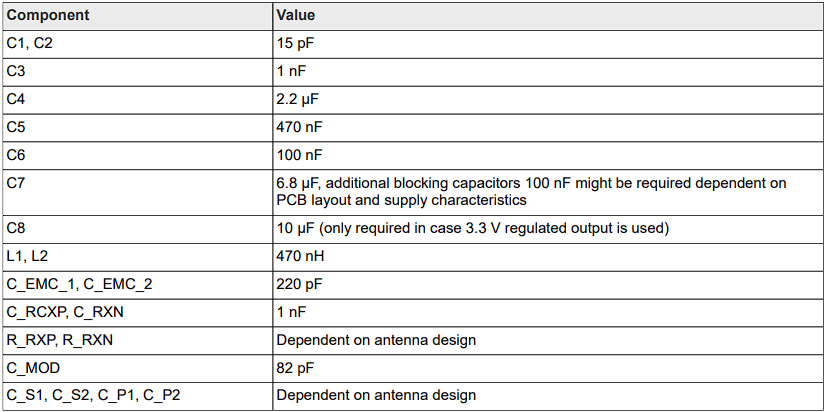
\includegraphics[width=0.7\textwidth]{images/design/pn5180mincompvalues}
    \caption{\centering Значения для элементов PN5180}
    \label{fig:pn5180mincompvalues}
\end{figure}

Также в открытом доступе находится принципиальная электрическая схема первой ревизии модуля PN5180 от производителя, которая и послужила основой для собственной электрической принципиальной схемы\cite{pn5180_schematic}.

% TODO: Подключение модулей

На основе всех вышеописанных сведений была спроектирована принципиальная схема разрабатываемой системы, показанная в приложении~Г.





\subsubsection{Макет аппаратной части системы}

В качестве МК для макета используется STM32F103C8T6 в составе отладочной платы Blue Pill, представленной на рисунке~\ref{fig:blue_pill}.

\begin{figure}[H]
    \centering
    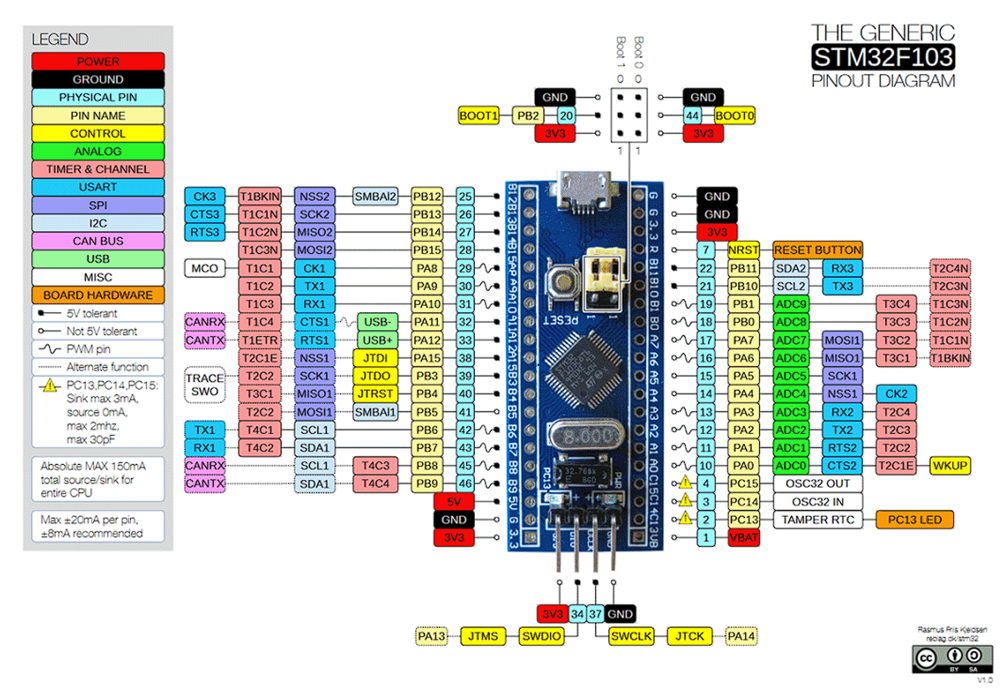
\includegraphics[width=0.8\textwidth]{images/design/blue_pill}
    \caption{\centering Отладочная плата Blue Pill с МК STM32F103C8T6}
    \label{fig:blue_pill}
\end{figure}

Сборка макета происходила в соответствии с принципиальной схемой из приложения~Г.
Макет представлен на рисунке~\ref{fig:maket}.

\begin{figure}[h]
    \centering
    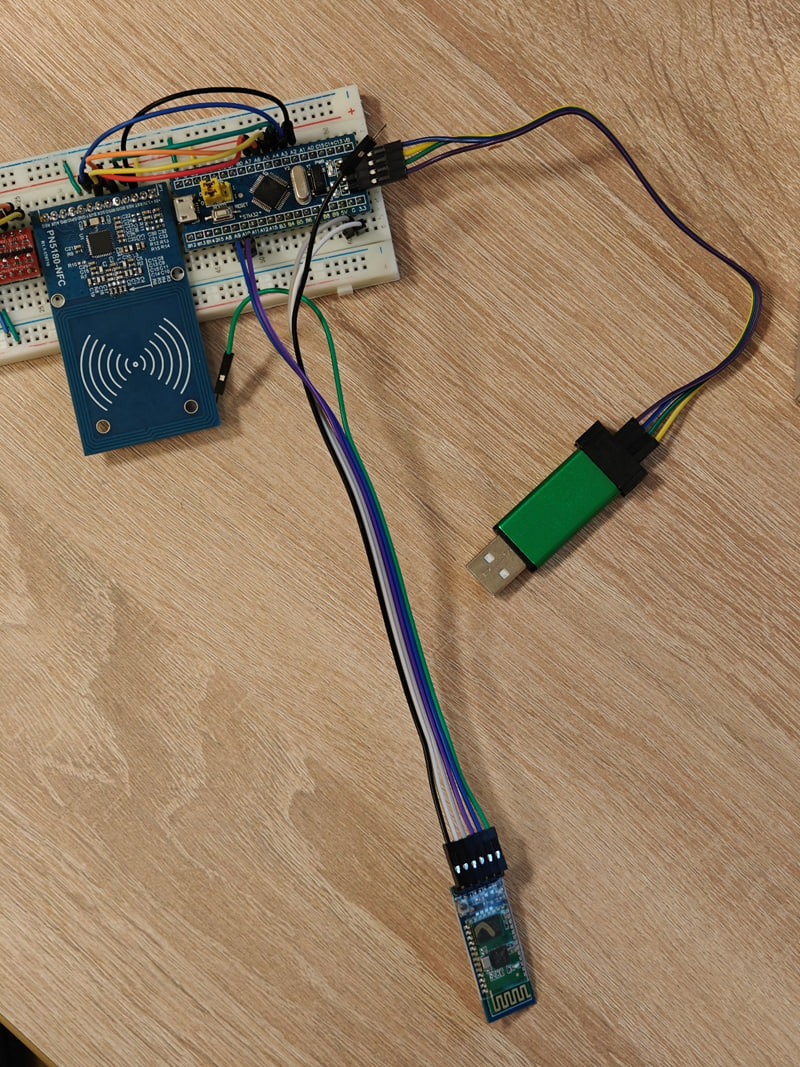
\includegraphics[width=0.5\textwidth]{images/design/maket}
    \caption{\centering Собранный макет устройства}
    \label{fig:maket}
\end{figure}

Для разработанного устройства-считывателя также был произведен расчет мощности.
Мощность, потребляемая разработанной схемой, складывается из мощностей, потребляемых всеми устройствами из ее состава.
Из документации используемых устройств получена информация, приведенная в таблице~\ref{tab:elements_power}.


Расчет максимальной мощности, потребляемой устройством, определяется по формуле:

$$
P_{max} = \sum_{i=1}^{k} U_i \cdot I_{i_{max}} \cdot n_i,
$$
где $U_i$~--- напряжение питания устройства, $I_{i_{max}}$~--- максимальный ток потребления, $n_i$~--- количество элементов в системе.

\begin{longtable}[l]{|
P{0.25\textwidth}|
P{0.3\textwidth}|
P{0.37\textwidth}|}

    \caption{Расчет потребляемой мощности}
    \label{tab:elements_power} \\
    \hline
    \textbf{Микросхема} &
    \textbf{Ток потребления, мА} &
    \textbf{Потребляемая мощность (при напряжении питания 5 В), мВт} \\
    \hline
    \endfirsthead

    \caption*{Продолжение таблицы~\ref{tab:elements_power}} \\
    \hline
    \textbf{Микросхема} &
    \textbf{Ток потребления, мА} &
    \textbf{Потребляемая мощность (при напряжении питания 5 В), мВт} \\
    \hline
    \endhead

    \hline
    \endfoot

    \hline
    \endlastfoot

    STM32F103C8T6 & 40 (активный режим) & 200 \\ \hline

    BC417143  & 30 (режим передачи) & 150 \\ \hline

    PN5180A0NH & 100 (при активном считывании) & 500 \\ \hline

    R1114-3.3 & 100 (с нагрузкой) & 500 \\ \hline

    RT9193-33 & 150 (с нагрузкой) & 750 \\ \hline

\end{longtable}

При напряжении питания 5 В максимальная мощность, потребляемая системой, будет равна 2,2 Вт.


\subsection{Разработка программной части системы}

\subsubsection{Программа считывателя бесконтактных платежных средств}

Алгоритм работы устройства:
\begin{enumerate}
    \item включение МК;
    \item настройка Bluetooth-модуля для подключения к мобильному устройству;
    \item установка соединения мобильного устройства и Bluetooth-модуля;
    \item получение команды от мобильного устройства о начале оплаты и суммы транзакции;
    \item включение и базовая настройка NFC-модуля микроконтроллером, начало поиска средства платежа;
    \item успешное или неудачное обнаружение и установка соединения со средством платежа средства платежа, передача результата обнаружения на мобильное устройство посредством Bluetooth;
    \item в случае успешного выполнения предыдущего этапа выполняется взаимодействие со средством платежа в соответствии алгоритмом Transaction Flow~\cite{book_mir};
    \item передача результата выполнения алгоритма Transaction Flow на мобильное устройство посредством Bluetooth;
\end{enumerate}

Успешный сценарий выполнения данного алгоритма приведен на диаграмме последовательностей, представленной в приложении~Е на листе~7.
На этом же листе представлен алгоритм успешного выполнения платежной операции с картой ПС <<МИР>>~--- MIR Transaction Flow~\cite{book_mir}.

В основу алгоритмов работы устройства легли алгоритмы, представленные на рисунках~\ref{fig:pcd_flow} и~\ref{fig:pcd_flow_2_picc_activation},~\ref{fig:transaction_flow_example} и~\ref{fig:kernel_transaction_flow}.
На основе них были разработаны несколько алгоритмов работы считывателя, в частности:

\begin{itemize}
    \item алгоритм выполнения платежной транзакции;
    \item алгоритм активации протокола ISO/IEC 14443--3;
    \item алгоритм активации протокола ISO/IEC 14443--4;
    \item алгоритм поиска платежных данных AFL.
\end{itemize}

Схема выполнения последнего алгоритма представлена на рисунке~\ref{fig:find_afl}.
Остальные диаграммы представлены в приложении~Е на листе~6.

\begin{figure}[H]
    \centering
    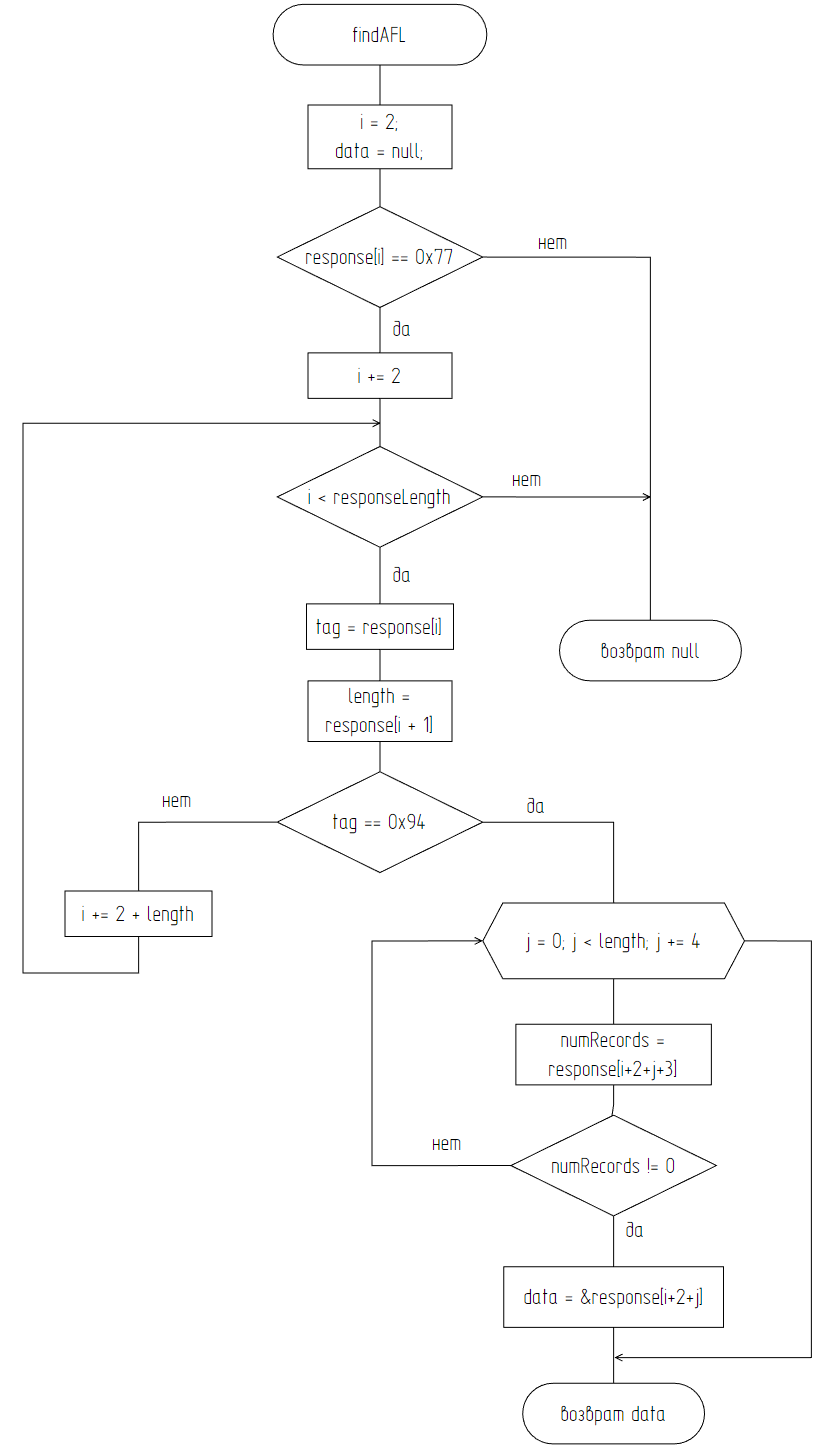
\includegraphics[width=0.7\textwidth]{images/design/find_afl}
    \caption{\centering Схема алгоритма поиска платежных данных AFL}
    \label{fig:find_afl}
\end{figure}


На рисунке~\ref{fig:find_afl} представлен алгоритм поиска значения тега Application File Locator (AFL), чтение которого является обязательным для формирования транзакции.
На основе найденного значения AFL формируется запрос чтения записи с карты~--- Read Record с указанием адреса, полученного в AFL.
Правила формирования следующие:

\begin{itemize}
    \item CLA = 0x00  - класс команды,
    \item INS = 0xB2 - тип инструкции (Read Record),
    \item P1 = Start - индекс первого байта,
    \item P2 = SFI|4 - второй параметр команды на основе SFI,
    \item Lc = 0x00 - ожидаемое количество байт в ответе (0 - любое).
\end{itemize}

Разработка программного обеспечения устройства происходила в среде STM32CubeIDE, предназначенной для разработки на микроконтроллерах серии STM32.
STM32 умеет производить компиляцию с файлов C и C++ с помощью gcc и g++.
В качестве основного языка программирования использовался C++, т.к. в отличие от C он предоставляет поддержку парадигмы объектно-ориентированного программирования.
Сама программа имеет модульный характер, на основе того, что в соответствие каждому аппаратному модулю (кроме МК) поставлен программный модуль, реализующий основные свойства и методы класса.

Настройка STM32F103C8T6 производилась с помощью графических средств STM32CubeIDE.
Пример такой настройки является настройка источника тактирования, представленная на рисунке~\ref{fig:stm_cube}.

\begin{figure}[h]
    \centering
    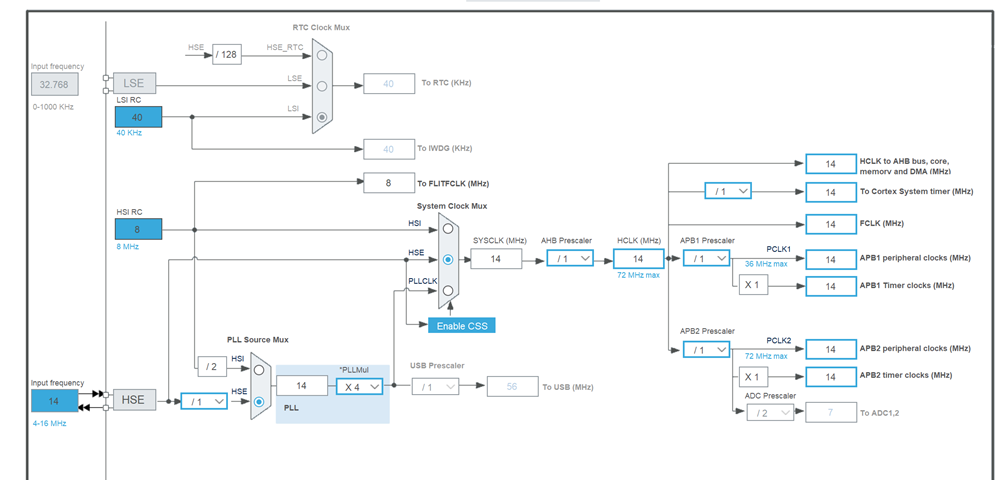
\includegraphics[width=1\textwidth]{images/design/stm_cube}
    \caption{\centering Настройка источника тактирования STM32F103C8T6}
    \label{fig:stm_cube}
\end{figure}

В качестве частоты используется 14 МГц для достижения максимальной скорости передачи данных с PN5180, который поддерживает максимальную скорость в 7 Мбит/с.
С помощью предделителя частоты SPI, равного 2, частота APB2 (именно к ней подключен SPI1) понижается до 7 МГц и 7 Мбит/с соответственно.
В приложении~Б приведены листинги со следующими фрагментами кода:
\begin{itemize}
    \item настройка SPI для подключения PN51804
    \item настройка USART для подключения Bluetooth-модуля HC-05.
\end{itemize}

Взаимодействие с PN5180 разделено на два класса PN5180 и PN5180ISO14443.
Первый описывает реализацию основных методов управления состоянием модуля, а второй реализует специфичные для стандарта ISO14443 методы работы, с помощью которых осуществляется взаимодействие NFC-модуля и платежного средства.
Примеры реализующих их процедур приведены в приложении~Б.


\subsubsection{Программа мобильного устройства}

В соответствии с требованиями ТЗ программа должна работать под управлением устройств с ОС Android версии 9 и выше.
Разрабатываемое программное обеспечение для мобильного устройства должно обеспечивать выполнение всех требуемых функций взаимодействия между считывателем бесконтактных карт и сервером банка-эквайера.
Управляющая программа будет работать на мобильном устройстве под управлением ОС Android и предоставлять пользовательский интерфейс для отслеживания состояния транзакции, её инициализации и получения результата.

Основные функции, выполняемые программой:
\begin{itemize}
    \item инициация взаимодействия между платежным средством (банковской картой или мобильным кошельком) и терминалом;
    \item взаимодействие с внешним сервером через протоколы HTTPS и REST API, с соблюдением требований стандарта PCI DSS;
    \item управление состоянием транзакции на основе данных, полученных от сервера и терминала, в соответствии с правилами EMV Transaction Processing и форматом сообщений ISO 8583;
    \item корректное завершение платежной операции, включая отображение результатов пользователю и передачу статуса транзакции.
\end{itemize}

Для начала транзакции программа использует данные, полученные от платежного терминала и карты.
Конкретный перечень полей определяется спецификой взаимодействия с каждой из поддерживаемых платежных систем.
При этом данные должны быть корректно интерпретированы и переданы на сервер эквайера через безопасное соединение.

Программа возвращает статус выполнения платежной операции в формате JSON, совместимом с REST API.
При этом максимальное время ожидания ответа от аппаратной части системы установлено на уровне 30 секунд, от внешнего сервера~--- 10 секунд.


Для реализации мобильного приложения была выбрана платформа Android SDK, так как она:
\begin{itemize}
    \item предоставляет полный доступ к низкоуровневым модулям, таким как Bluetooth и NFC;
    \item поддерживает современные протоколы шифрования и интеграции с REST API;
    \item обеспечивает гибкость в версионировании и обновлениях;
    \item использует Kotlin или Java, что позволяет писать чистый и понятный код, сохраняя высокую степень переносимости и производительности.
\end{itemize}

Для реализации сетевого взаимодействия используется Retrofit 2 и OkHttp, что обеспечивает:

\begin{itemize}
    \item удобную работу с REST API;
    \item поддержку TLS 1.2+;
    \item возможность добавления сложных заголовков, таких как авторизация и проверка целостности запросов.
\end{itemize}

Для тестирования и отладки применяются:

\begin{itemize}
    \item OkHttp Profiler — для контроля сетевых запросов;
    \item Mockk / JUnit — для автоматизированного тестирования бизнес-логики без необходимости использования реального терминала.
\end{itemize}

На основании процесса выполнения транзакции, описанного в спецификации EMV и алгоритма работы устройства-считывателя, был сформирован список необходимых экранов для основных сценариев использования приложения:
\begin{itemize}
    \item авторизация,
    \item выбор устройства,
    \item создание платежа,
    \item ожидание инициализации карты,
    \item успех/ошибка при инициализации карты,
    \item ввод PIN-кода,
    \item ввод подписи,
    \item успех/ошибка при выполнении платежа.
\end{itemize}

Формы всех экранов представлены на рисунке~\ref{fig:screens}.

\begin{figure}[h]
    \centering
    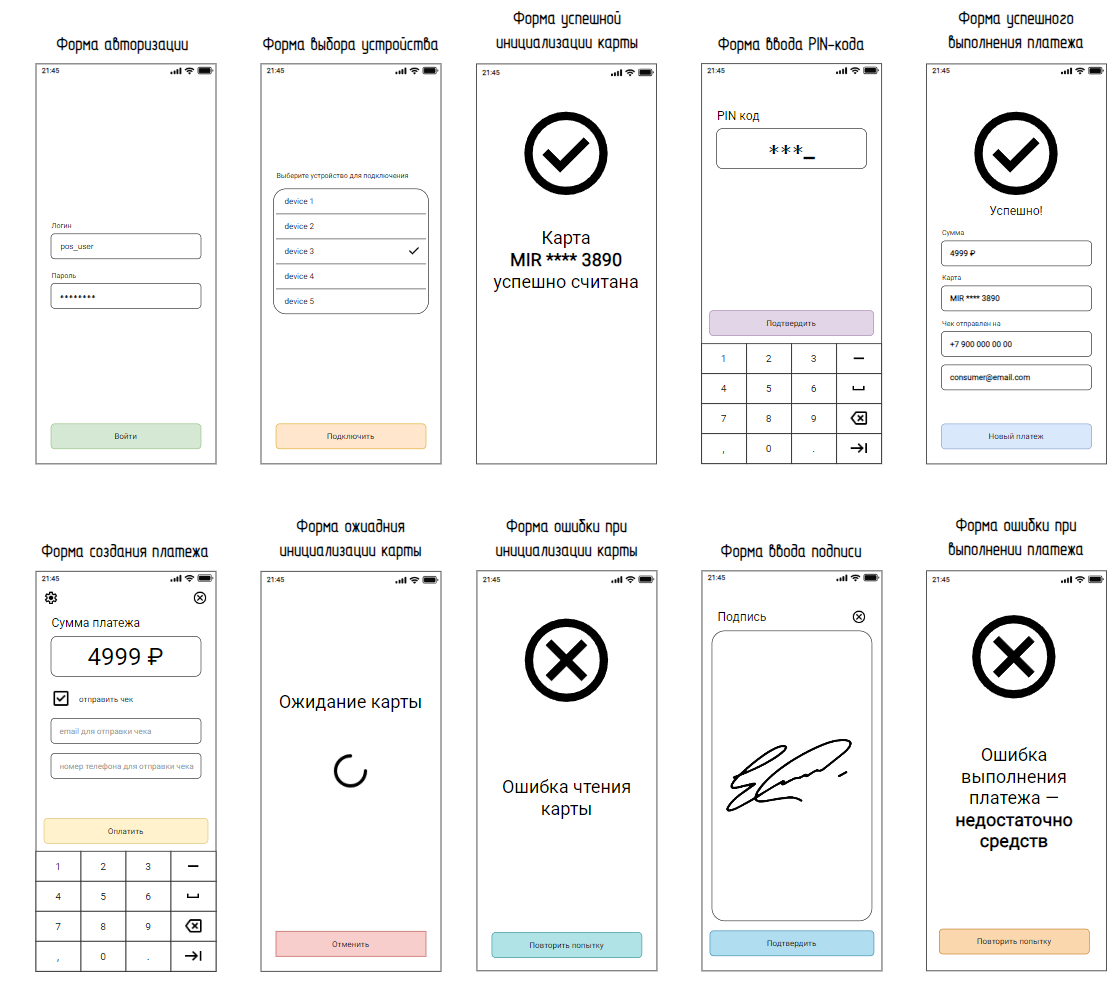
\includegraphics[width=0.9\textwidth]{images/design/screens}
    \caption{\centering Формы интерфейсов экранов приложения}
    \label{fig:screens}
\end{figure}

Экран авторизации должен иметь поля для ввода логина и пароля, и выполнять аутентификацию и авторизацию пользователя приложения с помощью введенных логина и пароля по нажатию кнопки <<Войти>>.
В случае успешной авторизации выполняется переход на экран выбора устройства для подключения.
В случае ошибки отображается сообщение об ошибке в нижней части экрана, поля ввода логина и пароля очищаются, пользователь может повторно ввести их и повторить попытку авторизации.

На экране выбора устройства отображаются все доступные для подключения Bluetooth-устройства.
При первом открытие экрана выполняется проверка наличия разрешений на подключение и обнаружение устройств поблизости посредством Bluetooth.
По нажатию на устройство должно выполняться сопряжение и/или подключение к выбранному устройству.
Если выбранное устройство~--- считыватель бесконтактных карт, то он сигнализирует (передает данные) об этом после подключения.
В случае успешного подключения к считывателю выполняется переход на экран создания платежа.
В случае неудачного подключения отображается сообщение об ошибке в нижней части экрана, пользователь может повторить попытку подключения к считывателю.

На экране создания платежа пользователь находится только при наличии активного подключения к считывателю.
Он может ввести сумму оплаты, а также, при необходимости, номер телефона и/или электронную почту для отправки электронного чека об операции.
По нажатию на кнопку <<Настройка>> происходит переход к экрану выбору устройств.
По нажатию на кнопку <<Очистить>> происходит очистка полей ввода суммы транзакции, полей ввода номера телефона и/или электронной почты.
По нажатию на кнопку <<Оплатить>> валидируются введеные пользователем данные, в случае их корректности отображается экран ожидания инициализации карты, в случае некорректности некорректные поля подсвечиваются, ошибка выводится на экран.

При переходе на экран ожидания инициализации карты на считыватель передается команда о необходимости запуска NFC-модуля, после его активации выполняется поиск бесконтактного платежного средства и взаимодействие с ним по спецификации ПС.
Если данные процессы выполнены успешно, то приложение получает от считывателя все необходимые данные для формирования платежной транзакции и отображает экран успешной инициализации карты, в противном случае~-- экран ошибки инициализации карты, на котором есть кнопка <<Повторить попытку>>, запускающая повторную инициализацию NFC-модуля и взаимодействие с картой.

Карта посредством считывателя может запросить дополнительную проверку в виде ввода PIN-кода держателем карты, в этом случае открывается экран ввода PIN-кода, на котором держатель карты может ввести кода от своей платежной карты.
Также проверка может запросить в виде ввода подписи держателя карты.
И PIN-код, и подпись отправляются в запросе в банк-эквайер посредством REST API с целью аутентификации держателя карты, банк отвечает статусом проверки держателя карты.

После успешной инициализации и прохождении проверок (либо их отсутствия) отправляется запрос в банк-эквайер посредством REST API с суммой операции и всеми необходимыми данными для выполнения платежа.
Банк-эквайер возвращает данные о результате выполнения платежной транзакции.
В зависимости от результата либо отображается экран успешного выполнения транзакции с информацией о транзакции, либо отображается экран с описанием произошедшей ошибки.
Оба экрана позволяют по нажатию кнопки перейти на экран создания платежа и создать новую платежную транзакцию.


На основе данного описания экранов был спроектирован граф состояний интерфейса, представленная на рисунке~\ref{fig:nav_graph}.

\begin{figure}[h]
    \centering
    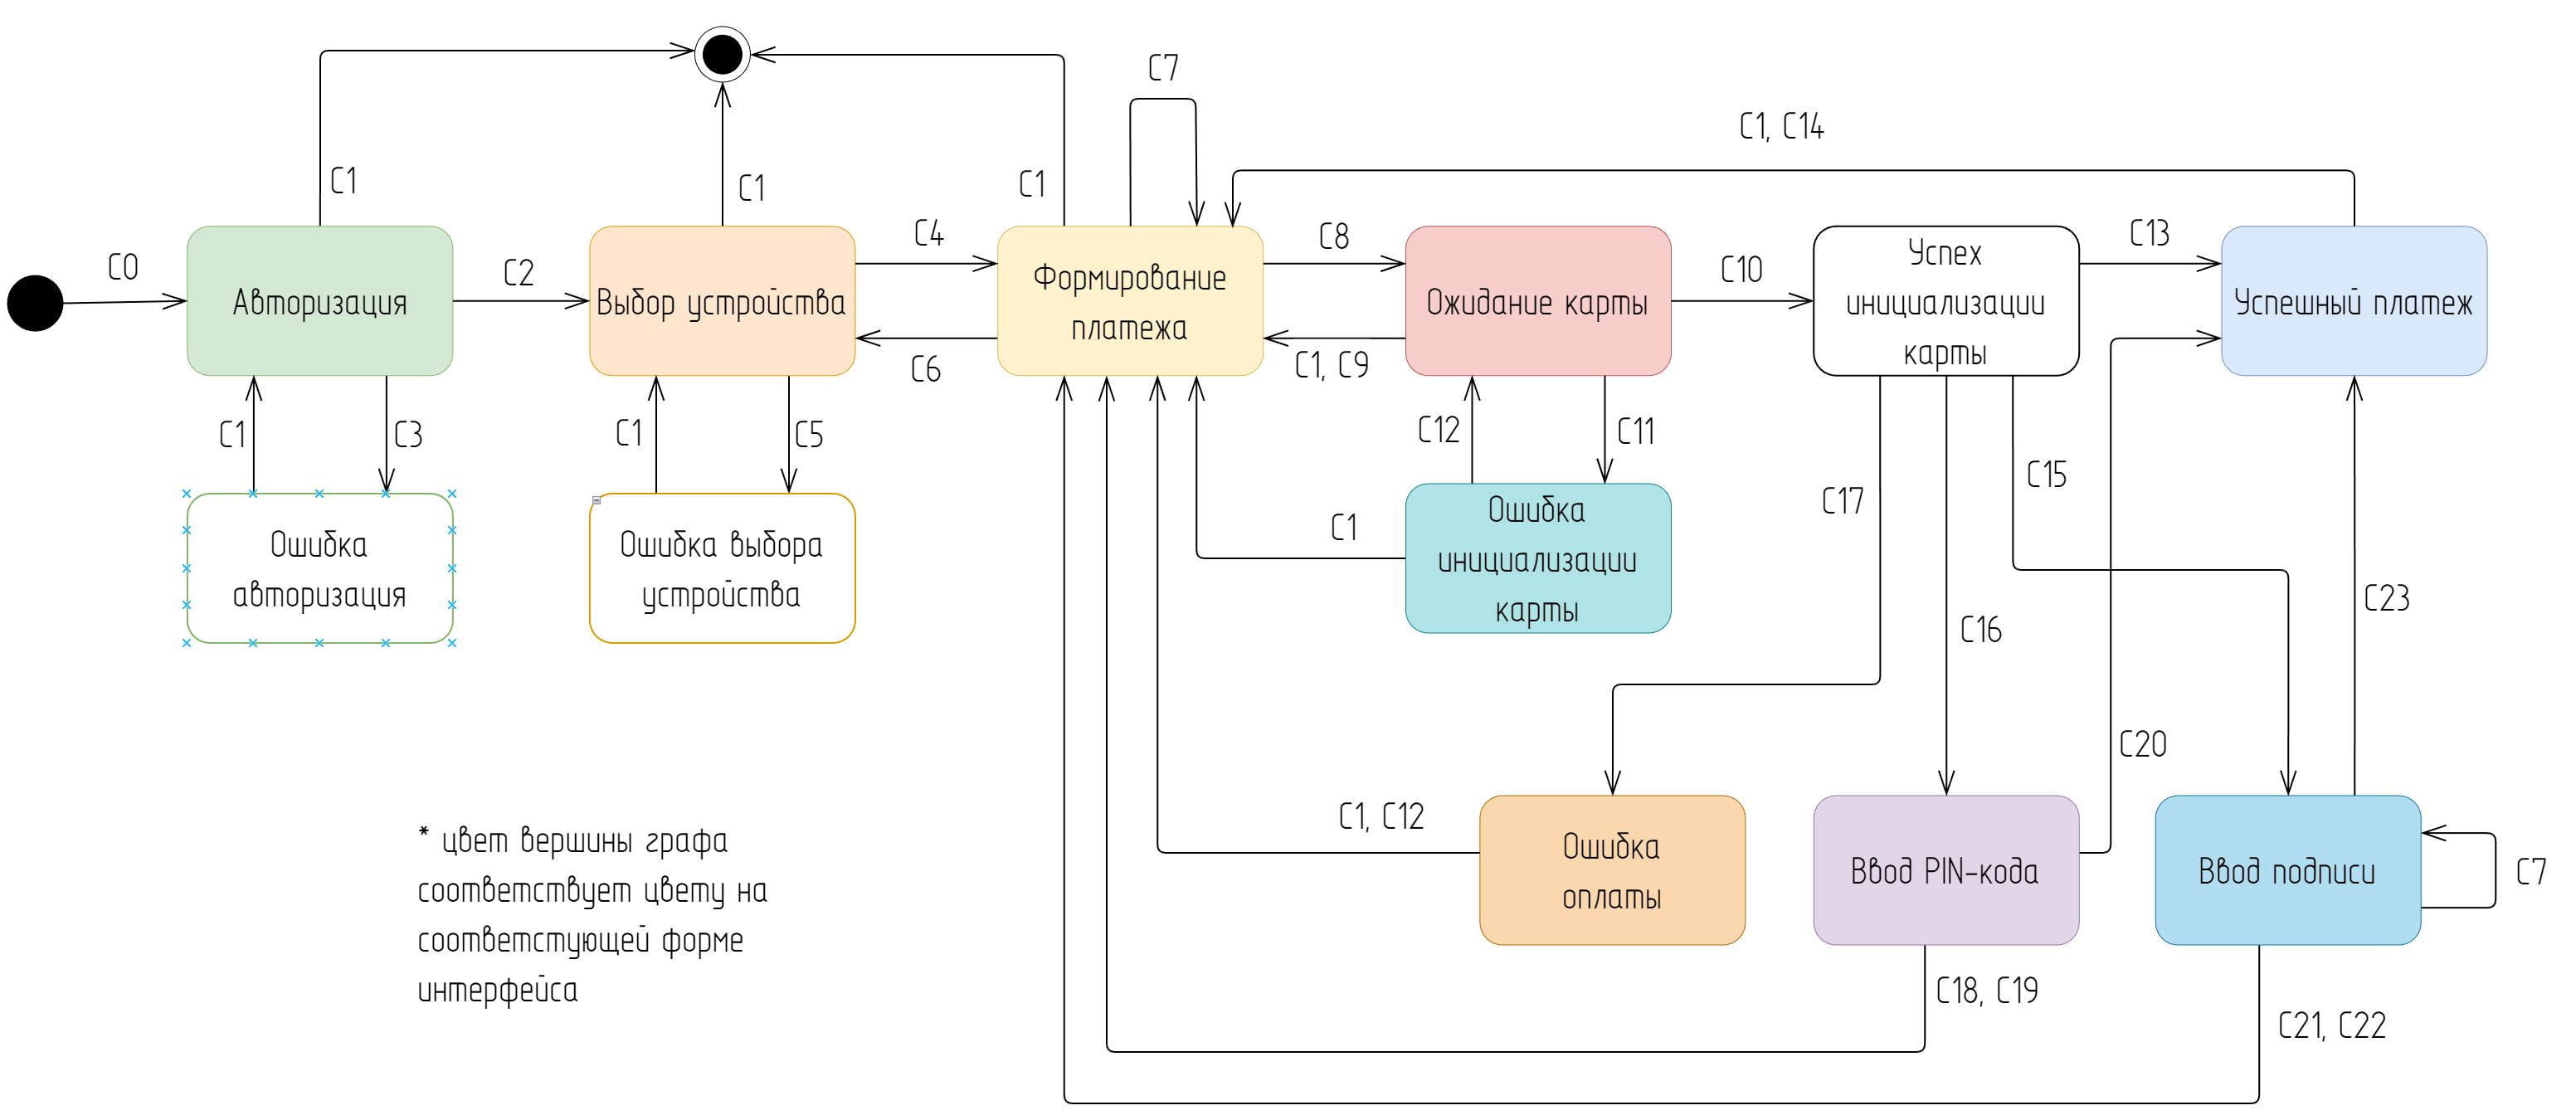
\includegraphics[width=1\textwidth]{images/design/nav_graph}
    \caption{\centering Граф состояний интерфейса}
    \label{fig:nav_graph}
\end{figure}

На котором введены следующие обозначения событий:
\begin{itemize}
    \item С0~--- открытие приложения,
    \item С1~--- нажатие системной кнопки <<Назад>>,
    \item С2~--- успешная авторизация после ввода данных и нажатия кнопки <<Войти>>,
    \item С3~--- ошибка авторизации после нажатия кнопки <<Войти>>,
    \item С4~--- успешное подключение к устройству после выбора устройства и нажатия <<Продолжить>>,
    \item С5~--- ошибка подключение к устройству после выбора устройства и нажатия <<Продолжить>>
    \item С6~--- нажатие иконки <<Настройки>>,
    \item С7~--- нажатие иконки <<Очистить данные>>,
    \item С8~--- нажатие кнопки <<Оплатить>>,
    \item С9~--- нажатие кнопки <<Отменить>>,
    \item С10~--- успешная инициализация карты,
    \item С11~--- ошибка при инициализации карты,
    \item С12~--- нажатие кнопки <<Повторить попытку>>,
    \item С13~--- успешное выполнение платежа,
    \item С14~--- нажатие кнопки <<Новый платеж>>,
    \item С15~--- запрос ввода подписи держателя карты,
    \item С16~--- запрос ввода PIN-кода держателя карты,
    \item С17~--- ошибка выполнения платежа,
    \item С18~--- ошибка проверки PIN-кода,
    \item С19~--- успешная проверка PIN-кода и ошибка при выполнении платежа,
    \item C20~--- успешная проверка PIN-кода и успешное выполнение платежа,
    \item С21~--- ошибка проверки подписи,
    \item С22~--- успешная проверка подписи и ошибка при выполнении платежа,
    \item С23~--- успешная проверка подписи и успешное выполнение платежа.
\end{itemize}


Для разрабатываемой программы, и системы в целом, была спроектирована диаграмма классов концептуального уровня.
Диаграмма представлена в приложении~Е на листе~5.

\subsection{Тестирование системы}

Для разработанного приложения было проведено структурное тестирование методом покрытия операторов.
Выполнения тестовых случаев и их проверка осуществлялось с помощью библиотек Mockk и JUnit для структурного и модульного тестирования.
Описание тестовых случаев, проверяющих работу устройства, перечислено в таблице~\ref{tab:mob_app_test_cases}.

\begin{longtable}[l]{| P{0.18\textwidth} | P{0.2\textwidth} | P{0.26\textwidth} | P{0.26\textwidth}|}

    \caption{Тестовые случаи структурного тестирования программной части системы}
    \label{tab:mob_app_test_cases} \\
    \hline
    \textbf{Тестируемый модуль} &
    \textbf{Описание теста} &
    \textbf{Ожидаемый результат} &
    \textbf{Полученный результат} \\
    \hline
    \endfirsthead

    \caption*{Продолжение таблицы~\ref{tab:mob_app_test_cases}} \\
    \hline
    \textbf{Тестируемый модуль} &
    \textbf{Описание теста} &
    \textbf{Ожидаемый результат} &
    \textbf{Полученный результат} \\
    \hline
    \endhead

    \hline
    \endfoot

    \hline
    \endlastfoot

    Авторизация &
    Ввод логина и пароля и нажатие кнопки <<Войти>> &
    Отправка REST API запроса авторизации &
    Запрос успешно отправлен \\
    \hline

    Авторизация &
    Проверка выполнения авторизации и последующего перехода на экран выбора устройства &
    Авторизация успешно выполнена, выполнен переход на экран выбора устройства &
    Успешная авторизация, переход выполнен \\
    \hline

    Авторизация &
    Проверка вывода ошибки при вводе некорректных данных авторизации &
    Отображение ошибки, очистка полей ввода &
    Ошибке отображена, поля очищены \\
    \hline

    Выбор устройства &
    Проверка отображения доступных Bluetooth-устройств &
    Успешная проверка доступа к Bluetooth и отображение доступных устройств &
    Доступ к Bluetooth есть, устройства поблизости отображаются \\
    \hline

    Выбор устройства &
    Подключение к считывателю бесконтактных карт из списка доступных устройств &
    При первом подключении запрашивается пароль, при повторном~--- успешное подключение &
    При первом подключении запрошен пароль, при повторном~--- успешное подключение  \\
    \hline

    Создание платежа &
    Отправка запроса инициализации карты после ввода корректной суммы и нажатия <<Оплатить>> &
    Отправка запроса на инициализацию карты &
    Данные корректно определены, переход на экран инициализации и запроса инициализации выполнены \\
    \hline

    Создание платежа &
    Отображение ошибки при вводе некорректной суммы и нажатии <<Оплатить>> &
    Подсветка поля ввода, вывод сообщения об ошибке &
    Поле подсвечено, ошибка отображена \\
    \hline

    Инициализация карты &
    Получение Bluetooth-сигнала об успешном обнаружении карты &
    Сигнал обнаружения получен по Bluetooth &
    Сигнала успешно получен \\
    \hline

    Инициализация карты &
    Поднесение несовместимого устройства или его отсутствие &
    Переход на экран ошибки инициализации карты по истечению 30 секунд &
    Переход на экран ошибки успешно осуществлен \\
    \hline

    Ввод PIN-кода &
    Поступление запроса на ввод PIN-кода по Bluetooth &
    Открытие экрана ввода PIN &
    Экран ввода успешно отображен \\
    \hline

    Ввод PIN-кода &
    Ввод некорректного PIN-кода &
    Подсветка поля ввода, вывод сообщения об ошибке &
    Поле выделено, ошибка отображена \\
    \hline

    Ввод PIN-кода &
    Онлайн проверка введенного PIN-кода &
    Отправка REST API запроса проверки PIN-кода &
    Запрос успешно отправлен \\
    \hline

    Ввод PIN-кода &
    Офлайн проверка введенного PIN-кода &
    Отправка запроса проверки PIN-кода по Bluetooth на считыватель &
    Запрос проверки успешно отправлен \\
    \hline

    Ввод подписи &
    Поступление запроса на ввод подписи держателя карты &
    Открытие экрана ввода подписи &
    Экран отображен \\
    \hline

    Ввод подписи &
    Отказ пользователя от ввода подписи &
    Отмена выполнения транзакции &
    Транзакция отменена, переход на экран ошибки \\
    \hline

    Успешное выполнение платежа &
    Получение ответа об успешном выполнении платежа &
    Отображение экрана успешной транзакции с данными о платеже &
    Экран успеха отображен, информация о платеже корректна \\
    \hline

    Модуль выполнения платежа &
    Получение ответа сервера об успешном выполнении платежа &
    Отображение экрана успешной транзакции с данными о платеже &
    Экран успеха отображен, информация о платеже корректна \\
    \hline

    Модуль выполнения платежа &
    Получение ответа сервера об ошибке при выполнении платежа &
    Отображение экрана ошибки, возможность начать новую транзакцию &
    Экран ошибки выполнения платежа \\
    \hline

    Модуль выполнения платежа &
    Обрыв связи с терминалом во время транзакции &
    Отображение ошибки выполнения платежа &
    Отображается экран ошибки выполнения платежа \\
    \hline
\end{longtable}


Тестирование ПО считывателя бесконтактных карт также проводилось методом покрытия операторов.
Была создана отдельная версия программного обеспечения МК, содержащую только код тестов.
Результатом тестирования является выполнение всех тестов и вывод отладочных сообщений после загрузки данного ПО на МК.
Значения в таблице~\ref{tab:test_cases_hardware} показывают корректность работы программного обеспечения МК.

\begin{longtable}[l]{| P{0.18\textwidth} | P{0.2\textwidth} | P{0.26\textwidth} | P{0.26\textwidth}|}

    \caption{Тестовые случаи структурного тестирования аппаратной части системы}
    \label{tab:test_cases_hardware} \\
    \hline
    \textbf{Тестируемый модуль} &
    \textbf{Описание теста} &
    \textbf{Ожидаемый результат} &
    \textbf{Полученный результат} \\
    \hline
    \endfirsthead

    \caption*{Продолжение таблицы~\ref{tab:test_cases_hardware}} \\
    \hline
    \textbf{Тестируемый модуль} &
    \textbf{Описание теста} &
    \textbf{Ожидаемый результат} &
    \textbf{Полученный результат} \\
    \hline
    \endhead

    \hline
    \endfoot

    \hline
    \endlastfoot

    USART интерфейс &
    Настройка USART интерфейса для подключения Bluetooth-модуля &
    USART успешно настроен на подключение Bluetooth-модуля &
    Параметры USART успешно изменены \\
    \hline

    Передача данных по USART &
    Отправка комбинации символов по USART &
    Корректная отправка комбинации символов на USART и их успешное получение &
    Комбинация успешно отправлена и получена \\
    \hline

    Получение данных по USART &
    Получение комбинации символов по USART &
    Комбинация символов передана и корректно получена &
    Комбинация успешно отправлена и получена \\
    \hline

    Конфигурация Bluetooth модуля &
    Проверка активации и корректности ответов на AT-команды настройки Bluetooth-модуля &
    Модуль Bluetooth должен корректно выполнять отправленные AT-команды и отвечать на них &
    Bluetooth-модуль активирован и корректно отвечает на команды \\
    \hline

    SPI интерфейс &
    Настройка SPI интерфейса для подключения NFC-модуля &
    SPI успешно настроен на подключение NFC-модуля &
    Параметры SPI успешно изменены \\
    \hline

    Передача данных по SPI &
    Отправка комбинации символов по SPI &
    Корректная отправка комбинации символов на SPI и их успешное получение &
    Комбинация успешно отправлена и получена \\
    \hline

    Получение данных по SPI &
    Получение комбинации символов по SPI &
    Комбинация символов передана и корректно получена &
    Комбинация успешно отправлена и получена \\
    \hline

    Активация NFC-модуля &
    Подача сигнала активации питания NFC-модуля &
    NFC-модуль активируется и отвечает на отправленные команды &
    NFC-модуль успешно активирован и отвечает на запрос версии модуля \\
    \hline

    Включение РЧ-поля NFC-модуля &
    Отправка команды включения РЧ-поля NFC-модуля &
    Происходит переход в состояние включенного РЧ-поля &
    Выполнен переход в состояние включенного РЧ-поля \\
    \hline

    Установка значений регистра NFC-модуля &
    Отправка команды изменение значения регистра NFC-модуля &
    В регистре NFC-модуля находится обновленное значение &
    Значение в регистре соответствует измененному \\
    \hline

    Запись значения в память NFC-модуля &
    Отправка команды изменение значения по определенному адресу в памяти NFC-модуля &
    Записанное значение находится в памяти NFC-модуля по указанному в команде адресу &
    Значение по указанному адресу в памяти соответствует записанному \\
    \hline

\end{longtable}

Тестирование работы системы проводилось в соответствии с технологией, описанной в разделе~\ref{sec:technolog} ручным способом.
Была протестирована реакция системы на поднесение бесконтактной платежный карты к NFC-модулю.
Если средство платежа обнаруживалось и распознавалось корректно, то устройство выводило текст, информирующий об успешной идентификации карты и ее уникальный идентификатор UID.
В случае возникновения ошибки на последовательный порт отправлялись сообщения с описанием проблемы, множественный вывод в различных местах позволял определять причину неисправности.

Проверка корректной работы проходила по следующему сценарию:
\begin{enumerate}
    \item в мобильном приложении создается платежная операция, активируется считыватель средств платежа, к нему подносится карта <<МИР>> с поддержкой бесконтактной оплаты;
    \item ожидаемая реакция: успешное считывание карты и получение необходимых для оплаты данных;
    \item полученный результат: установлено соединение с картой по стандарту ISO/IEC 14443 в результате которого получен UID карты, также в результате выполнения MIR Transaction Flow успешно получены данные в бинарном формате TLV (Tag--Length--Value) для формирования запроса на платежный сервер банка-эквайера.
\end{enumerate}

На рисунке ~\ref{fig:test_success} показаны данные, выведенные в результате логирования работы считывателя на Serial Monitor при успешной работе системы.

\begin{figure}[H]
    \centering
    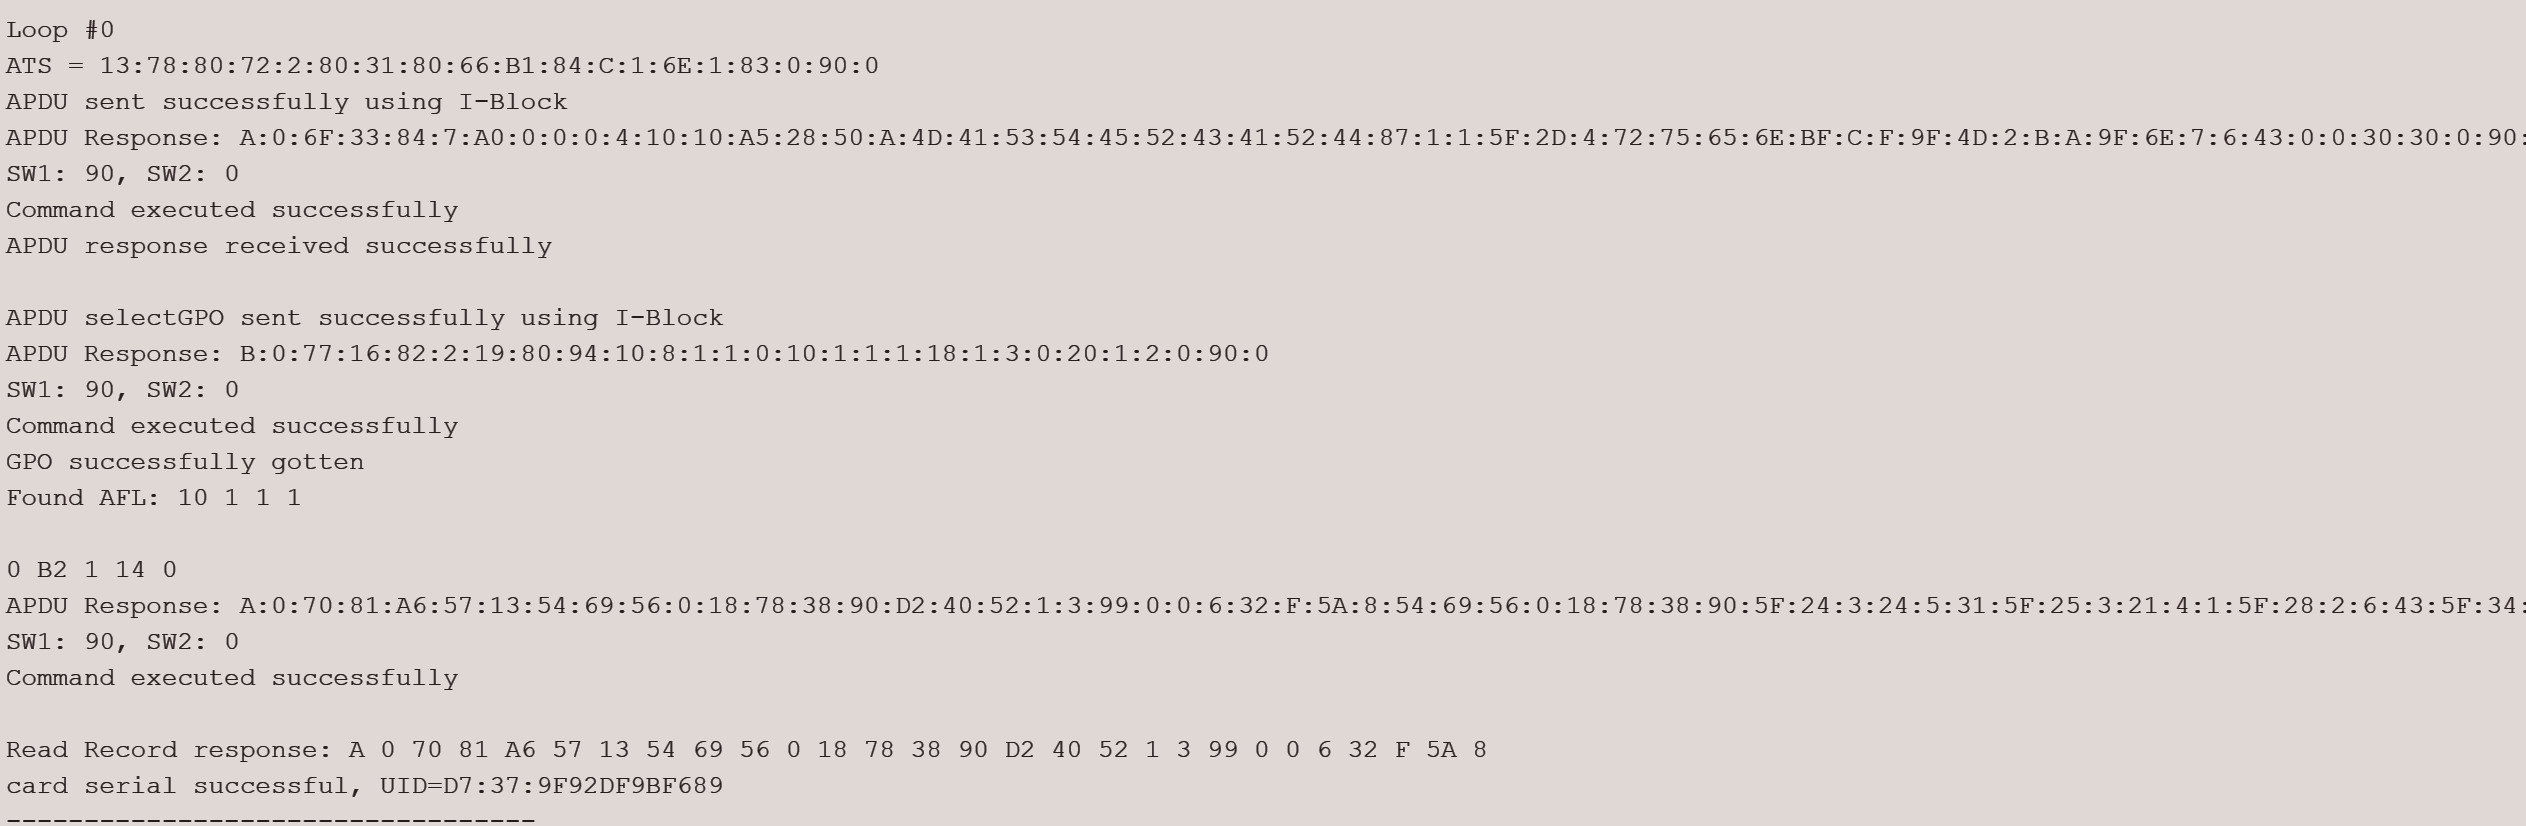
\includegraphics[width=1\textwidth]{images/design/test_success_white}
    \caption{\centering Результат успешного тестирования системы}
    \label{fig:test_success}
\end{figure}


%Тестирование интеграции частей системы происходило

	%\newpage
% 1. Разработать технологию тестирования системы
% 2. Разработать технологии развертывания и использования системы

\section{Разработка технологий развертывания и тестирования системы}

Согласно техническому заданию выпускной квалификационной работы бакалавра требуется разработать технологию тестирования работы системы, а также выполнить комплекс проверок для интеграции программной и аппаратной частей.
Это позволяет убедиться в корректности обмена данными между мобильным приложением, считывателем бесконтактных карт и сервером банка-эквайера.

\subsection{Технология тестирования работы системы}
Технология тестирования разработанной программно-аппаратной системы включает последовательность действий, направленных на проверку основных функциональных модулей:

\begin{itemize}
	\item подключение к считывателю по Bluetooth;
	\item активация и взаимодействие с NFC-картой;
	\item обмен APDU-командами;
	\item интеграция с сервером банка через REST API;
	\item обработка ошибок и отображение результатов транзакции пользователю.
\end{itemize}

Для реализации технологии тестирования были определены следующие этапы:

\begin{enumerate}
	\item подготовка макета устройства и установка прошивки — включает загрузку актуальной версии ПО на микроконтроллер и проверку его запуска;
	\item настройка среды эмуляции платежной транзакции — имитируется поведение терминала и сервера банка, чтобы протестировать все возможные сценарии: успех, ошибка связи, некорректный UID, неверная криптограмма, блокировка карты и другие;
	\item проверка интеграции с мобильным приложением — выполняется полный цикл тестирования от подключения к устройству до получения результата операции;
	\item отладка и анализ логов — используется система логирования (Logcat для Android, Serial Monitor для микроконтроллера), чтобы выявить возможные проблемы на уровне протоколов и интерфейсов.
\end{enumerate}

Процесс тестирования представлен в виде алгоритма, включающего три основных режима:

\begin{itemize}
	\item модульное тестирование компонентов (отдельные модули ПО и аппаратуры);
	\item интеграционное тестирование — проверка взаимодействия между мобильным приложением, считывателем и сервером;
	\item системное тестирование — полный сценарий использования системы от авторизации пользователя до завершения транзакции.
\end{itemize}

\subsection{Тестирование аппаратной части системы}
В рамках данной ВКР был создан макет устройства, реализующий следующие функции:

\begin{itemize}
	\item чтение данных с бесконтактной карты по стандартам ISO/IEC 14443--3 и ISO/IEC 14443--4;
	\item передача данных на мобильное приложение по каналу Bluetooth;
	\item инициализация транзакции и генерация управляющих команд;
	\item защита передаваемых данных с использованием сессионных ключей и шифрования.
\end{itemize}

Для автоматизации тестирования и активации аппаратной части системы был реализован скрипт, представленный в листинге~\ref{code:update_firmware}, принимающий параметры:

\begin{itemize}
	\item адрес NFC-ридера;
	\item режим тестирования (NFC / Bluetooth / Power);
	\item количество повторов.
\end{itemize}


\begin{singlespacing}
	\small
	\captionsetup{labelsep=endash, justification=raggedright, singlelinecheck=off}
	\lstinputlisting[language=bash, label=code:update_firmware, caption={Скрипт обновления прошивки МК}]{code/test.sh}
\end{singlespacing}


Этот скрипт позволяет провести серию тестов, сохраняя результаты в JSON-файл, который затем может быть использован для анализа надёжности и производительности.



\subsection{Тестирование программной части системы}
Мобильное приложение, реализованное под ОС Android, было протестировано на корректность выполнения следующих функций:

\begin{itemize}
	\item авторизация пользователя;
	\item подключение к считывателю;
	\item формирование запроса на оплату;
	\item отправка данных через REST API;
	\item обработка ответов от сервера и отображение результата.
\end{itemize}

Был разработан набор автономных тестовых сценариев , использующих Mock-объекты и подмену ответов от сервера , чтобы проверить все варианты развития транзакции без прямого доступа к реальному банку.


Для упрощения тестирования и отладки была создана демонстрационная среда , в которую входят:

\begin{itemize}
	\item скрипты эмуляции ответов от сервера эквайера;
	\item утилиты Bluetooth- и NFC-тестирования.
\end{itemize}

\subsection{Интеграционное тестирование}
\label{subsec:test_integr}
Для проверки интеграции программной и аппаратной частей системы был разработан полный сценарий тестирования, включающий:

\begin{enumerate}
	\item включение устройства и его инициализация;
	\item поиск и подключение через Bluetooth к считывателю;
	\item ввод суммы и запуск транзакции;
	\item считывание UID, активация карты и обмен APDU-командами;
	\item передача данных на сервер;
	\item получение ответа и отображение результата пользователю.
\end{enumerate}

Все эти этапы были протестированы в различных условиях:

\begin{itemize}
	\item при слабом сигнале Bluetooth;
	\item при отсутствии или плохом качестве соединения с сервером.
\end{itemize}

В результате тестирования не выявлено критических ошибок, связанных с потерей данных или нарушением целостности транзакции.
Все этапы обмена данными между программной и аппаратной частью выполняются корректно и соответствуют требованиям безопасности, установленными в техническом задании.






%
%\vspace{2mm}
%В результате выполнения технологической части разработки системы были разработаны технологии:
%\begin{enumerate}
%	\item развертывания и использования системы~--- на их основе было создано руководство по эксплуатации системы (приложение Д);
%	\item тестирования системы~--- на основе данной технологии были определены цели, а также методы тестирования компонентов системы и проведено ее тестирования, результаты которого описаны в предыдущей главе.
%\end{enumerate}


	%\newpage

\centeredsection{ЗАКЛЮЧЕНИЕ}
\addcontentsline{toc}{section}{ЗАКЛЮЧЕНИЕ}

В ходе выполнения выпускной работы бакалавра был проведен анализ предметной области ...


	\newpage

\begin{center}
	\phantomsection
	\section*{\centering СПИСОК ИСПОЛЬЗОВАННЫХ ИСТОЧНИКОВ}
	\addcontentsline{toc}{section}{СПИСОК ИСПОЛЬЗОВАННЫХ ИСТОЧНИКОВ}
\end{center}

\printbibliography[heading=none]

%\makebibliography

	\setcounter{pagecount}{\value{page}-1}
	\setcounter{figurescount}{\value{figure}} % Новый счетчик, потому что в приложениях обнуляю список рисунков

% TODO поменять номера страниц в приложениях
	\newpage

\begin{center}
  \myAppendix{Техническое задание}  

  \pdfximage{docs/tz.pdf}
  на \the\pdflastximagepages\ листах
\end{center}

\newpage

\ifthenelse{\boolean{test_vkr}}{

%  
\includepdf[pages=1]{docs/tz.pdf} % титульный лист ТЗ без подписи
  \begin{figure}[H]
    \centering
    
\includegraphics[height=0.95\textheight]{docs/tz v2-01.png} % титульного листа ТЗ без подписи для прохождения тестВКР
  \end{figure}
  \newpage
}{
  
\includepdf[pages=1]{docs/podpis/tz_titul.pdf} % подписанный титульный лист ТЗ
}

\newpage

\includepdf[pages=2-]{docs/tz v2.pdf} % ТЗ

% \addtocounter{page}{11}


\newpage

\begin{center}
   \myAppendix{Фрагменты исходного кода}
   на 7 листах
\end{center}
\newpage

\ifthenelse{\boolean{website_upload}}{
  \includepdf{docs/source_title.pdf}
}{
  \ifthenelse{\boolean{test_vkr}}{
    \begin{figure}[H]
      \centering
      
\includegraphics[height=0.95\textheight]{docs/title_source_code.png}
    \end{figure}
    \newpage
  }{
    \bmstutitleAppendix{Фрагменты исходного кода}
  }
}

\begin{singlespacing}
	\small
	\captionsetup{labelsep=endash, justification=raggedright, singlelinecheck=off}
	\lstinputlisting[language=c++, label=code:spi_init, linerange={1-50}, caption={Фрагмент настройки подключения PN5180 к МК}]{code/spi_init.cpp}
\end{singlespacing}



\pagebreak
\begin{singlespacing}
	\small
	\captionsetup{labelsep=endash, justification=raggedright, singlelinecheck=off}
	\lstinputlisting[language=c++, label=code:init, caption={Настройка подключения HC-05 к МК}]{code/init.cpp}
\end{singlespacing}



\begin{singlespacing}
    \small
    \captionsetup{labelsep=endash, justification=raggedright, singlelinecheck=off}
    \lstinputlisting[language=c++, label=code:control, linerange={1-22}, caption={Реализация управляющих методов для PN5180}]{code/control.cpp}
\end{singlespacing}
\pagebreak
{
    \noindent \small Продолжение листинга~\ref{code:control}
}
\vspace{-\baselineskip}
\begin{singlespacing}
    \small
    \captionsetup{labelsep=endash, justification=raggedright, singlelinecheck=off}
    \lstinputlisting[language=c++, linerange={23-64}, firstnumber=23, aboveskip=3mm]{code/control.cpp}
\end{singlespacing}
{
    \noindent \small Продолжение листинга~\ref{code:control}
}
\vspace{-\baselineskip}
\begin{singlespacing}
    \small
    \captionsetup{labelsep=endash, justification=raggedright, singlelinecheck=off}
    \lstinputlisting[language=c++, linerange={65-}, firstnumber=65, aboveskip=3mm]{code/control.cpp}
\end{singlespacing}



%\begin{singlespacing}
%	\small
%	\captionsetup{labelsep=endash, justification=raggedright, singlelinecheck=off}
%	\lstinputlisting[language=c++, label=code:read_serial, linerange={1-50}, caption={Чтение UID карты и проверки его корректности}]{code/read_serial.cpp}
%\end{singlespacing}
%{
%    \noindent \small Продолжение листинга~\ref{code:read_serial}
%}
%\vspace{-\baselineskip}
%\begin{singlespacing}
%    \small
%    \captionsetup{labelsep=endash, justification=raggedright, singlelinecheck=off}
%    \lstinputlisting[language=c++, linerange={51-}, firstnumber=51, aboveskip=3mm]{code/read_serial.cpp}
%\end{singlespacing}

% \addtocounter{page}{5}


\newpage

\ifthenelse{\boolean{website_upload}}{
	\phantomsection
    % TODO replace file
    
\includepdf{appendices/podpis/func_preview.pdf}

	\addtocounter{appendixNum}{1}
	\addcontentsline{toc}{section}{ПРИЛОЖЕНИЕ \Asbuk{appendixNum}.~Схема электрическая функциональная}
	\setcounter{figure}{0}
	\renewcommand{\thefigure}{\Asbuk{appendixNum}\arabic{figure}}
}{
    \begin{center}
        \myAppendix{Схема электрическая функциональная}
        на 1 листе
        \newpage
    \end{center}
}

\begin{center}
  \begin{figure}[H]
    \centering
    \fbox{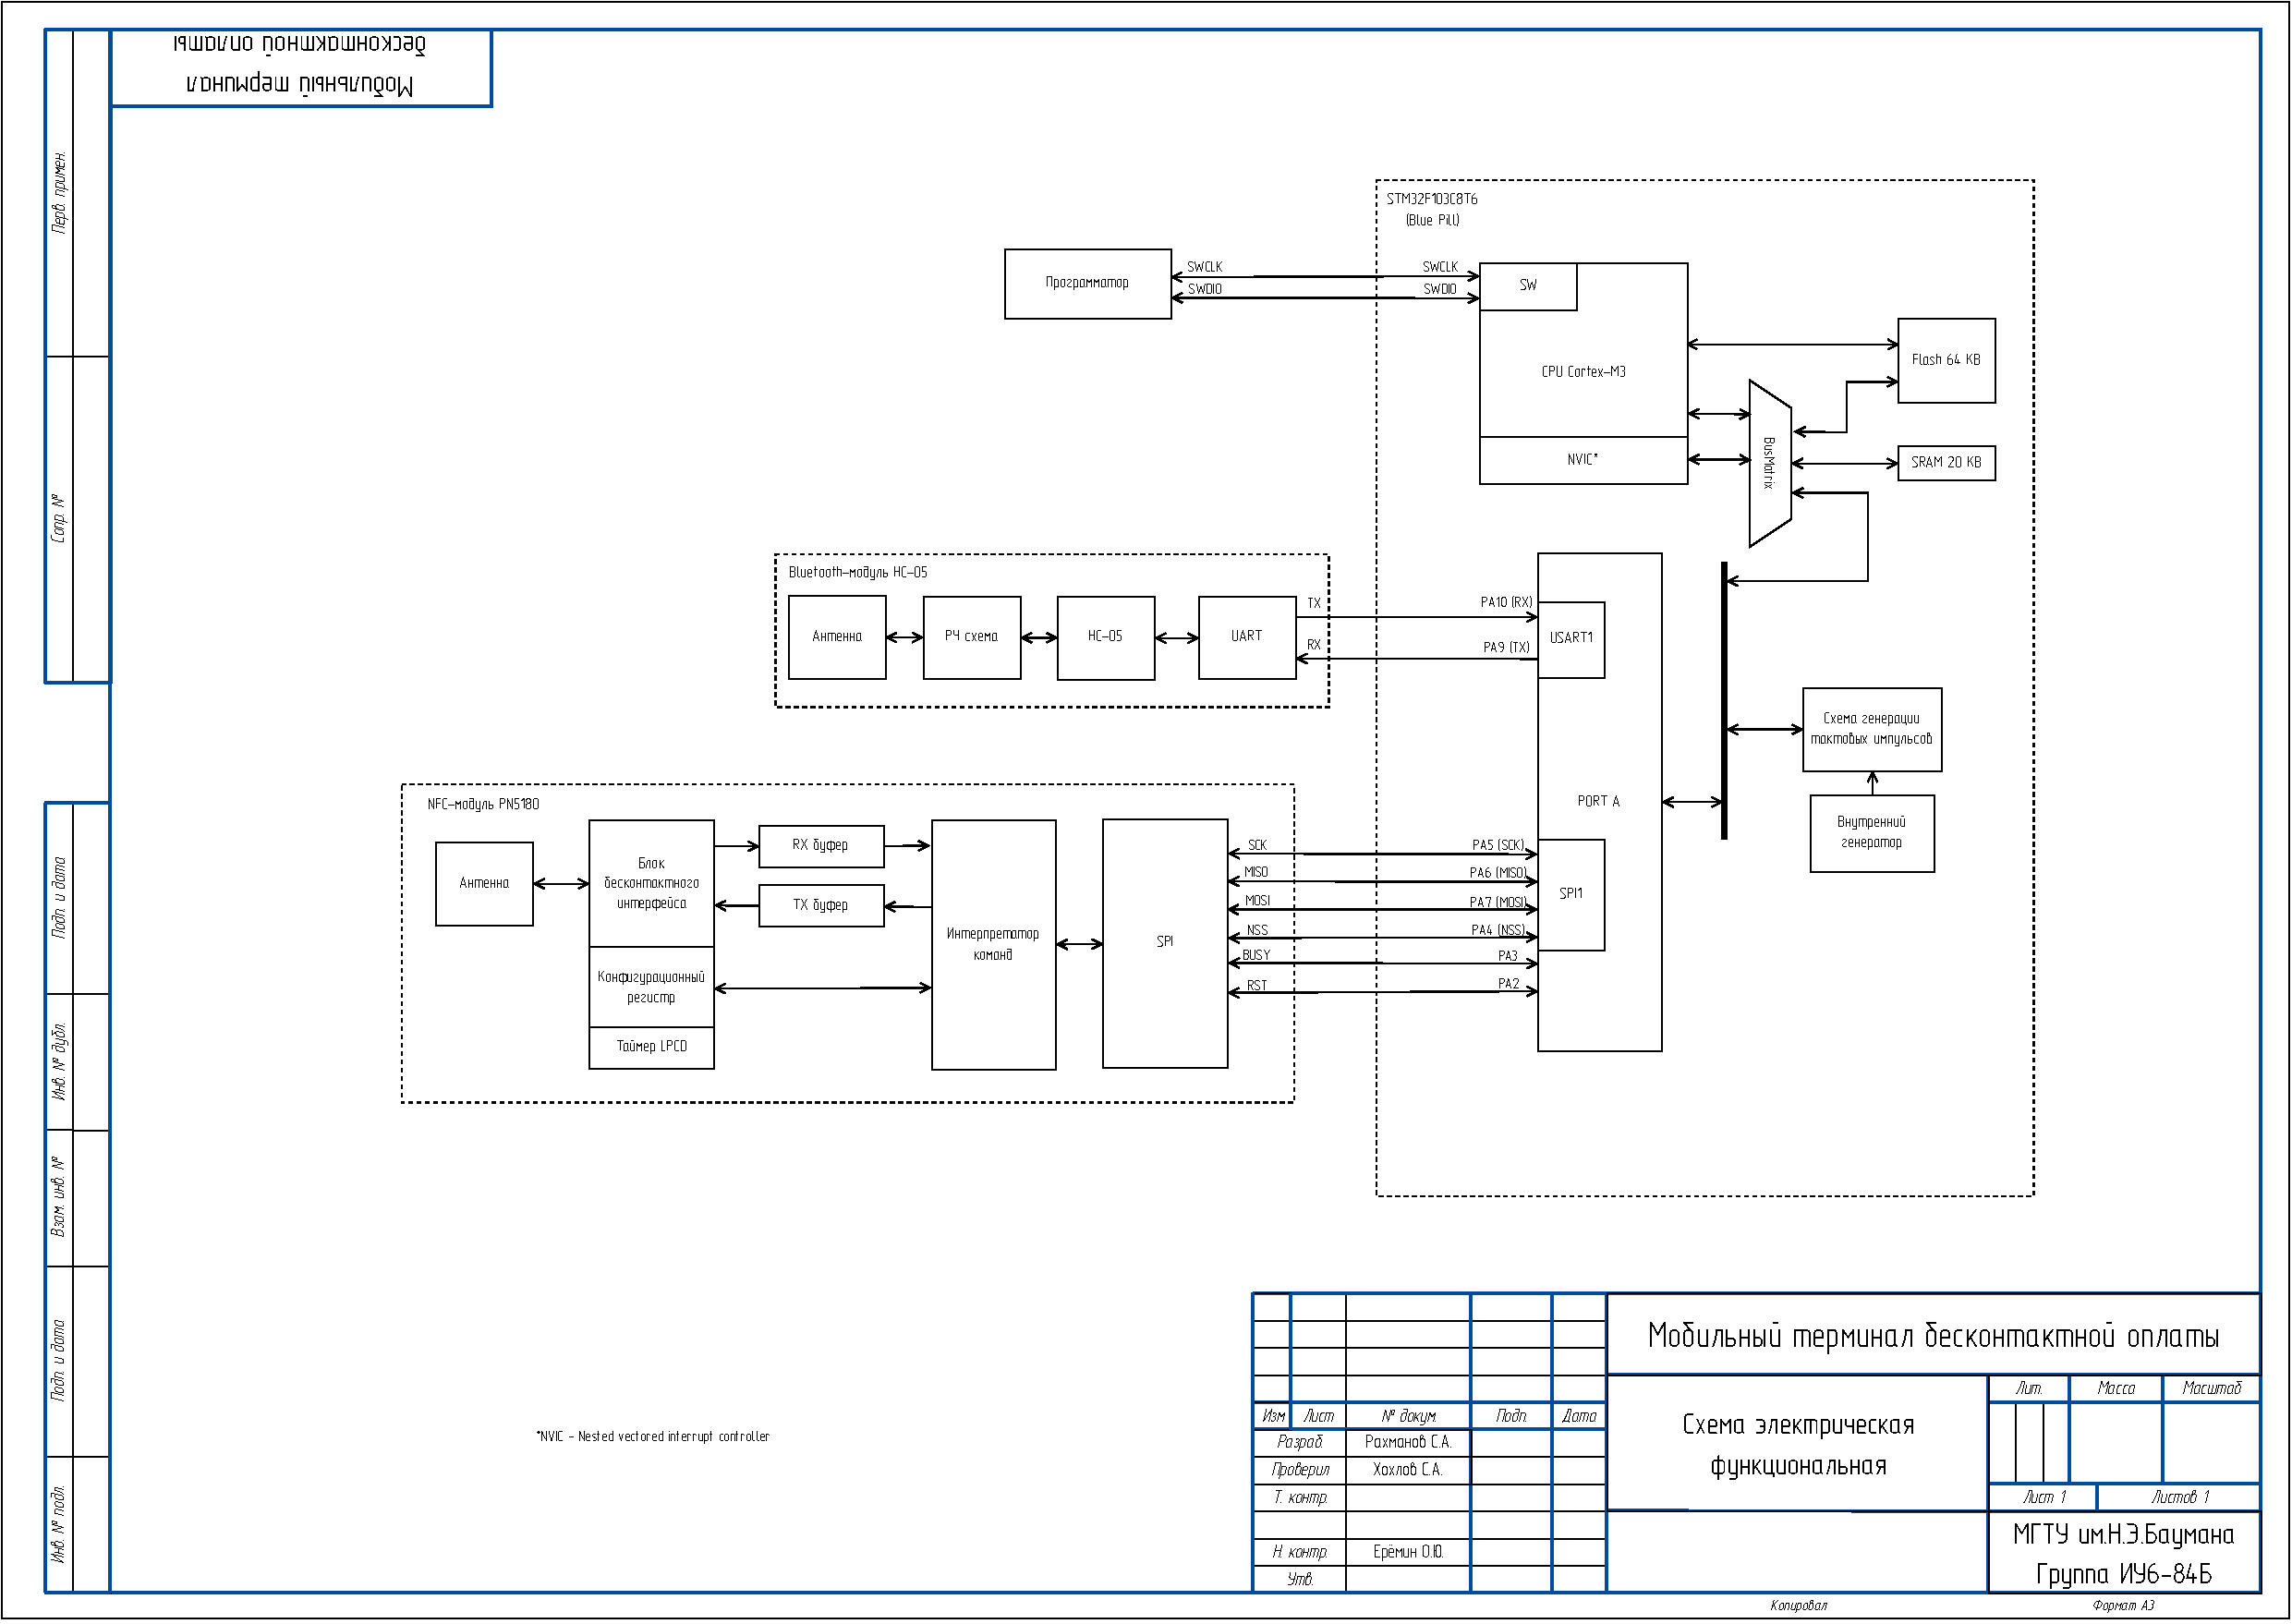
\includegraphics[angle=90, height=0.9\textheight]{appendices/func.pdf}}
    \caption*{\centering Рисунок \Asbuk{appendixNum}1 --- Схема электричекая функциональная}
  \end{figure}
\end{center}

% \addtocounter{page}{1}


\newpage

\ifthenelse{\boolean{website_upload}}{
	\phantomsection
  \includepdf{docs/appendix_principal.pdf}

	\addtocounter{appendixNum}{1}
	\addcontentsline{toc}{section}{ПРИЛОЖЕНИЕ \Asbuk{appendixNum}.~Схема электрическая принципиальная}
	\setcounter{figure}{0}
	\renewcommand{\thefigure}{\Asbuk{appendixNum}\arabic{figure}}
}{
    \begin{center}
        \myAppendix{Схема электрическая принципиальная}
        на 1 листе
        \newpage
    \end{center}
}

\begin{center}
  % TODO: экспортировать принципиалку по нормальному (по границе листа, а не формата а1)
  \begin{figure}[H]
    \centering
    \fbox{\includegraphics[angle=90, height=0.9\textheight]{appendices/schemas_princip.pdf}}
    \caption*{\centering Рисунок \Asbuk{appendixNum}1 --- Схема электричекая принципиальная}
  \end{figure}
\end{center}

% \addtocounter{page}{1}


\newpage

\begin{center}
    \myAppendix{Перечень элементов}
    на 2 листах
\end{center}
\newpage

\ifthenelse{\boolean{website_upload}}{
    \newpage
    \includepdf[pages=1-2]{appendices/podpis/elements.pdf}
}{
    \setcounter{figure}{0}
    \renewcommand{\thefigure}{\Asbuk{appendixNum}\arabic{figure}}

    \begin{figure}[H]
        \centering
        \includegraphics[height=0.95\textheight]{appendices/Спецификация Лист 1.jpg}
        \caption{Перечень элементов аппаратной части системы}
    \end{figure}

    \begin{figure}[H]
        \centering
        \includegraphics[height=0.95\textheight]{appendices/Спецификация Лист 2.jpg}
        \caption{Перечень элементов аппаратной части системы (окончание)}
    \end{figure}
}


% \addtocounter{page}{2}


%\input{src/9e_operating_manual}

%\newpage

\ifthenelse{\boolean{website_upload}}{
	\phantomsection
    % TODO replace file
    \includepdf{appendices/podpis/schemas_preview.pdf}

	\addtocounter{appendixNum}{1}
	\addcontentsline{toc}{section}{ПРИЛОЖЕНИЕ \Asbuk{appendixNum}.~Копии листов графической части}
	\setcounter{figure}{0}
	\renewcommand{\thefigure}{\Asbuk{appendixNum}\arabic{figure}}
}{
    \begin{center}
      \myAppendix{Копии листов графической части.}
    \end{center}

    \begin{enumerate}
      \item Структурная схема системы;
      \item Схема электрическая принципиальная аппаратной части системы;
      \item Граф состояний интерфейса;
      \item Формы интерфейса;
      \item Диаграммы классов программного обеспечения;
      \item Схемы алгоритмов модулей (подпрограмм);
      \item Диаграмма последовательностей системы.
    \end{enumerate}
}

{
\setcounter{figure}{0}
\renewcommand{\thefigure}{\Asbuk{appendixNum}\arabic{figure}}

\newpage
\begin{figure}[H]
    \centering
    \fbox{\includegraphics[angle=90,height=0.9\textheight]{appendices/schemas-1.pdf}}
    \caption{Структурная схема системы}
\end{figure}

\begin{figure}[H]
    \centering
    \fbox{\includegraphics[angle=90,height=0.9\textheight]{appendices/schemas_princip.pdf}}
    \caption{Схема электрическая принципиальная аппаратной части системы}
\end{figure}

\begin{figure}[H]
    \centering
    \fbox{\includegraphics[angle=90,height=0.9\textheight]{appendices/schemas-2.pdf}}
    \caption{Граф состояний интерфейса}
\end{figure}

\begin{figure}[H]
    \centering
    \fbox{\includegraphics[angle=90,height=0.9\textheight]{appendices/schemas-3.pdf}}
    \caption{Формы интерфейса}
\end{figure}

\begin{figure}[H]
    \centering
    \fbox{\includegraphics[angle=90,height=0.9\textheight]{appendices/schemas-4.pdf}}
    \caption{Диаграммы классов программного обеспечения}
\end{figure}

\begin{figure}[H]
    \centering
    \fbox{\includegraphics[angle=90,height=0.9\textheight]{appendices/schemas-5.pdf}}
    \caption{Схемы алгоритмов модулей (подпрограмм)}
\end{figure}

\begin{figure}[H]
    \centering
    \fbox{\includegraphics[angle=90,height=0.9\textheight]{appendices/schemas-6.pdf}}
    \caption{Диаграммма последовательностей системы}
\end{figure}
}
% \addtocounter{page}{6}



	\setcounter{appendixcount}{\value{appendixNum}}

\end{document}

